% ==============================================================================
% BLM3810 Biyoenformatiğe Giriş - Proje Raporu
% ==============================================================================
\documentclass[12pt,a4paper,oneside]{report}

\usepackage{iftex}
\ifPDFTeX
  \usepackage[T1]{fontenc}
  \usepackage[utf8]{inputenc}
  \IfFileExists{XCharter.sty}{\usepackage{XCharter}}{}
\else
  \usepackage{fontspec}
  \IfFontExistsTF{XCharter}{\setmainfont{XCharter}}{\setmainfont{Latin Modern Roman}}
\fi
\usepackage[shorthands=off,turkish]{babel}
\usepackage{geometry}
\geometry{a4paper,left=35mm,right=25mm,top=25mm,bottom=25mm}
\usepackage{graphicx}
\usepackage{titlesec}
\usepackage{tocloft}
\usepackage{booktabs}
\usepackage{longtable}
\usepackage{array}
\usepackage{tabularx}
\usepackage[justification=centering,labelsep=space,labelfont=bf]{caption}
\usepackage{float}
\usepackage{enumitem}
\usepackage{xcolor}
\usepackage{amsmath}
\usepackage{amssymb}
\usepackage[hidelinks]{hyperref}
\usepackage{setspace}
\usepackage{ragged2e}

\renewcommand{\contentsname}{İÇİNDEKİLER}
\renewcommand{\listfigurename}{ŞEKİL LİSTESİ}
\renewcommand{\listtablename}{TABLO LİSTESİ}
\renewcommand{\figurename}{Şekil}
\renewcommand{\tablename}{Tablo}

% --- Yazı tipi ---
\onehalfspacing
\setlength{\parindent}{0pt}
\setlength{\parskip}{6pt}

% --- Satır kırma toleransı (Türkçe tireleme yok) ---
\tolerance=2000
\emergencystretch=2em
\hbadness=4000

% --- YTÜ proje şablonuna yakın bölüm başlığı stili ---
\renewcommand{\chaptername}{}
\titleformat{\chapter}[display]
  {\bfseries\Large}
  {\filleft\bfseries\fontsize{30}{30}\selectfont\thechapter}
  {12pt}
  {\vspace{-1.15em}\filleft\Large\MakeUppercase}
  [\vspace{0.5em}\titlerule]
\titleformat{name=\chapter,numberless}[display]
  {\bfseries\Large}
  {}
  {0pt}
  {\filleft\Large\MakeUppercase}
  [\vspace{0.5em}\titlerule]
\titlespacing*{\chapter}{0pt}{12pt}{24pt}

\titleformat{\section}
  {\bfseries\large}{\thesection}{1em}{}[\vspace{-1.2em}]
\titleformat{\subsection}
  {\bfseries\normalsize}{\thesubsection}{1em}{}[\vspace{-1.2em}]

% --- İçindekiler ve liste stilleri ---
\renewcommand{\cftchapfont}{\bfseries}
\renewcommand{\cftchappagefont}{\bfseries}
\renewcommand{\cftchapleader}{\cftdotfill{\cftdotsep}}
\setlength{\cftbeforechapskip}{6pt}
\setlength{\cftchapnumwidth}{1.6em}
\setlength{\cftsecnumwidth}{2.4em}
\setlength{\cftsubsecnumwidth}{3.2em}
\renewcommand{\cftfigpresnum}{\figurename\enspace}
\renewcommand{\cftfigaftersnum}{}
\setlength{\cftfignumwidth}{4.5em}
\renewcommand{\cfttabpresnum}{\tablename\enspace}
\renewcommand{\cfttabaftersnum}{}
\setlength{\cfttabnumwidth}{4.5em}

% --- Kısaltma listesi stili ---
\newlist{abbrv}{itemize}{1}
\setlist[abbrv,1]{label=,labelwidth=3.2cm,align=parleft,itemsep=0.1\baselineskip,leftmargin=!}

\graphicspath{{figures/}{uploads/}{../results/figures/}}
\captionsetup{font=small}
\renewcommand{\thefigure}{\thechapter.\arabic{figure}}
\renewcommand{\thetable}{\thechapter.\arabic{table}}

% Sayfa numarası başlık hizası
\usepackage{fancyhdr}
\fancyhf{}
\cfoot{\thepage}
\renewcommand{\headrulewidth}{0pt}
\fancypagestyle{plain}{%
  \fancyhf{}%
  \cfoot{\thepage}%
  \renewcommand{\headrulewidth}{0pt}%
}
\pagestyle{fancy}

\begin{document}
\hypersetup{pageanchor=false}

% ==============================================================================
% KAPAK SAYFASI
% ==============================================================================
\begin{titlepage}
\begin{center}
\large
\textbf{T.C.\\[2pt]
YILDIZ TEKNİK ÜNİVERSİTESİ\\[2pt]
BİLGİSAYAR MÜHENDİSLİĞİ BÖLÜMÜ}

\vspace*{0.5cm}
\IfFileExists{uploads/ytu_logo.png}
  {\includegraphics[width=0.25\textwidth]{uploads/ytu_logo.png}}
  {\vspace{3.2cm}}

\vspace*{1.5cm}
\Large
\parbox[][2.2cm][c]{1.0\textwidth}{
\centering
\textbf{GEN İFADESİ VERİ SETLERİ ÜZERİNDE\\[6pt]
GEN ANALİZLERİ VE MAKİNE ÖĞRENMESİ İLE\\[6pt]
HEPATOSELLÜLER KARSİNOM SINIFLANDIRMASI}
}

\vspace{2.4cm}
\large
\textbf{BLM3810 BİYOENFORMATİĞE GİRİŞ\\[4pt] DÖNEM PROJESİ}

\vspace{2cm}

\vfill
\large
Dr. S. Sevgi TURGUT ÖGME

\vspace{1.5cm}
\large
Haziran, 2026
\end{center}
\end{titlepage}

% ==============================================================================
% ÖN SAYFALAR (roman numbering)
% ==============================================================================
\pagenumbering{roman}
\hypersetup{pageanchor=true}

\chapter*{İÇİNDEKİLER}
\renewcommand\contentsname{\vspace{-3.6em}}
\tableofcontents
\clearpage

% --- KISALTMA LİSTESİ ---
\chapter*{KISALTMA LİSTESİ}
\addcontentsline{toc}{chapter}{KISALTMA LİSTESİ}
\vspace{-0.3em}
\begin{abbrv}
\item[AUC] Area Under the Curve (ROC Eğrisi Altındaki Alan)
\item[Cox] Cox Orantılı Hazardlar Modeli
\item[DGE] Differential Gene Expression (Diferansiyel Gen İfadesi)
\item[GEO] Gene Expression Omnibus
\item[GO] Gene Ontology
\item[GS] Gene Significance (Gen Anlamlılığı)
\item[HCC] Hepatocellular Carcinoma (Hepatosellüler Karsinom)
\item[HVG] Highly Variable Genes (Yüksek Varyanslı Genler)
\item[kME] Module Membership (Modül Üyeliği)
\item[logFC] Log2 Fold Change
\item[OS] Overall Survival (Genel Sağkalım)
\item[PCA] Principal Component Analysis (Temel Bileşen Analizi)
\item[RFS] Recurrence-Free Survival (Nükssüz Sağkalım)
\item[ROC] Receiver Operating Characteristic
\item[SVM] Support Vector Machine (Destek Vektör Makinesi)
\item[WGCNA] Weighted Gene Co-expression Network Analysis
\end{abbrv}
\clearpage

% --- ŞEKİL LİSTESİ ---
\chapter*{ŞEKİL LİSTESİ}
\renewcommand\listfigurename{\vspace{-3.2em}}
\addcontentsline{toc}{chapter}{ŞEKİL LİSTESİ}
\listoffigures
\clearpage

% --- TABLO LİSTESİ ---
\chapter*{TABLO LİSTESİ}
\renewcommand\listtablename{\vspace{-3.2em}}
\addcontentsline{toc}{chapter}{TABLO LİSTESİ}
\listoftables
\clearpage

% ==============================================================================
% ANA İÇERİK
% ==============================================================================
\pagenumbering{arabic}

% ------------------------------------------------------------------------------
\chapter{GİRİŞ}

Kanser, hücre büyümesinin kontrolden çıkması sonucu ortaya çıkan ve dünya genelinde önde gelen ölüm nedenlerinden biri olan bir hastalık grubudur. Kanser dokularında, normal dokulara göre birçok genin ifade düzeyinde belirgin değişiklikler görülebilir.
Bazı genler aşırı aktive olurken, bazıları baskılanır. Bu farkların belirlenmesi, kanserle ilişkili genleri bulmak ve hastalığın tanı ya da seyri hakkında bilgi verebilecek çözümler geliştirmek açısından önemlidir.

Bu projede, Hepatosellüler Karsinom (HCC), karaciğer kanseri hastalığına ait gen ifadesi verileri üzerinde temel biyoinformatik analizler uygulanmış ve elde edilen biyolojik bulgular makine öğrenmesi tabanlı bir sınıflandırma problemine dönüştürülmüştür.

\section{Projenin Amacı}

Bu çalışmanın amacı, gen ifadesi veri setleri üzerinde diferansiyel gen ifadesi analizi, survival analizi, WGCNA ve GO enrichment analizleri uygulamak ve elde edilen sonuçları kullanarak tümör ile normal dokuyu ayırt edebilen makine öğrenmesi modelleri geliştirmektir. Proje iki aşamadan oluşmaktadır:

\begin{itemize}[leftmargin=*]
\item \textbf{Birinci aşama:} Veri seti seçimi, ön işleme, diferansiyel gen ifadesi analizi, survival analizi, WGCNA ve GO enrichment analizleri.
\item \textbf{İkinci aşama:} Farklı özellik seçimi/çıkarımı stratejileri kullanılarak makine öğrenmesi ile tümör/normal doku sınıflandırması.
\end{itemize}

\section{Veri Seti Bilgileri}

Çalışmada kullanılan veri seti NCBI GEO veritabanından elde edilen GSE76427 erişim numaralı hepatosellüler karsinom veri setidir. Veri setine ait temel bilgiler Tablo~\ref{tab:dataset} içinde özetlenmiştir.

\begin{table}[H]
\centering
\caption{GSE76427 veri seti özellikleri}
\label{tab:dataset}
\begin{tabularx}{\textwidth}{l X}
\toprule
\textbf{Özellik} & \textbf{Değer} \\
\midrule
GEO Erişim Numarası & GSE76427 \\
Hastalık & Hepatosellüler Karsinom (Karaciğer Kanseri) \\
Organizma & Homo sapiens \\
Toplam Örnek & 167 \\
Tümör Dokusu & 115 primer HCC örneği \\
Non-Tümör Dokusu & 52 komşu non-tümör karaciğer dokusu \\
Sınıflandırma Etiketi & Tümör vs Non-Tümör \\
Yaş Aralığı & 14--93 \\
Cinsiyet & 93 Erkek / 22 Kadın (klinik metadata’ya sahip 115 tümör örneği için)\\
Sağkalım Verisi & OS: 115 örnek, 23 ölüm olayı; RFS: 108 örnek, 48 tekrarlama olayı \\
\bottomrule
\end{tabularx}
\end{table}

Veri seti, tümör ve non-tümör olmak üzere iki karşılaştırılabilir sınıf içermesi, survival metadata bilgisine sahip olması ve kanser evresinin sınıflandırma etiketi olarak kullanılmaması nedeniyle proje gereksinimlerini karşılamaktadır.

\section{Rapor Organizasyonu}

Rapor, giriş bölümünü takip eden yedi ana bölümden oluşmaktadır:

\begin{itemize}
    \item İkinci bölümde veri ön işleme ve normalizasyon adımları açıklanmaktadır.
    \item Üçüncü bölümde diferansiyel gen ifadesi analizi ele alınmaktadır.
    \item Dördüncü bölümde survival analizi ve Cox modeli sunulmaktadır.
    \item Beşinci bölümde WGCNA ağ analizi incelenmektedir.
    \item Altıncı bölümde GO enrichment analizi değerlendirilmektedir.
    \item Yedinci bölümde makine öğrenmesi ile tümör/normal doku sınıflandırması yapılmaktadır.
    \item Sekizinci bölümde çalışmanın genel sonuçları özetlenmektedir.
\end{itemize}


% ------------------------------------------------------------------------------
\chapter{VERİ SETİ VE ÖN İŞLEME}

\section{Veri İndirme}

Veri seti, NCBI GEO veritabanından indirilmiştir. Analizde, GSE76427 veri setine ait normalize edilmemiş ham gen ifade verileri kullanılmıştır. Bu dosyada her prob için ifade değeri ve tespit güvenilirliğini gösteren Detection P-value bilgisi bulunmaktadır.

Ham veri başlangıçta 47.322 prob ve 167 örnekten oluşmaktadır. Tüm ifade değerleri pozitif olduğu için veriye log2 dönüşümü uygulanabilmiştir.


\section{Normalizasyon}

Ham verilere sırasıyla aşağıdaki adımlar uygulanmıştır:

\begin{enumerate}[leftmargin=*]
\item \textbf{Log2 dönüşümü:} Geniş aralığı sıkıştırmak ve dağılımı simetrikleştirmek için kullanılmıştır.
\item \textbf{Quantile normalizasyon:} Örnekler arasındaki teknik farklılıkları azaltmak ve gen ifade değerlerini karşılaştırılabilir hale getirmek için uygulanmıştır.
\end{enumerate}

Normalizasyon öncesi ve sonrası örnek dağılımları Şekil~\ref{fig:boxnorm} ve Şekil~\ref{fig:densnorm} ile gösterilmiştir. Normalizasyon sonrası tüm örneklerin medyan ve dağılımları hizalanmıştır.

\begin{figure}[H]
\centering
\begin{minipage}{0.49\textwidth}
\centering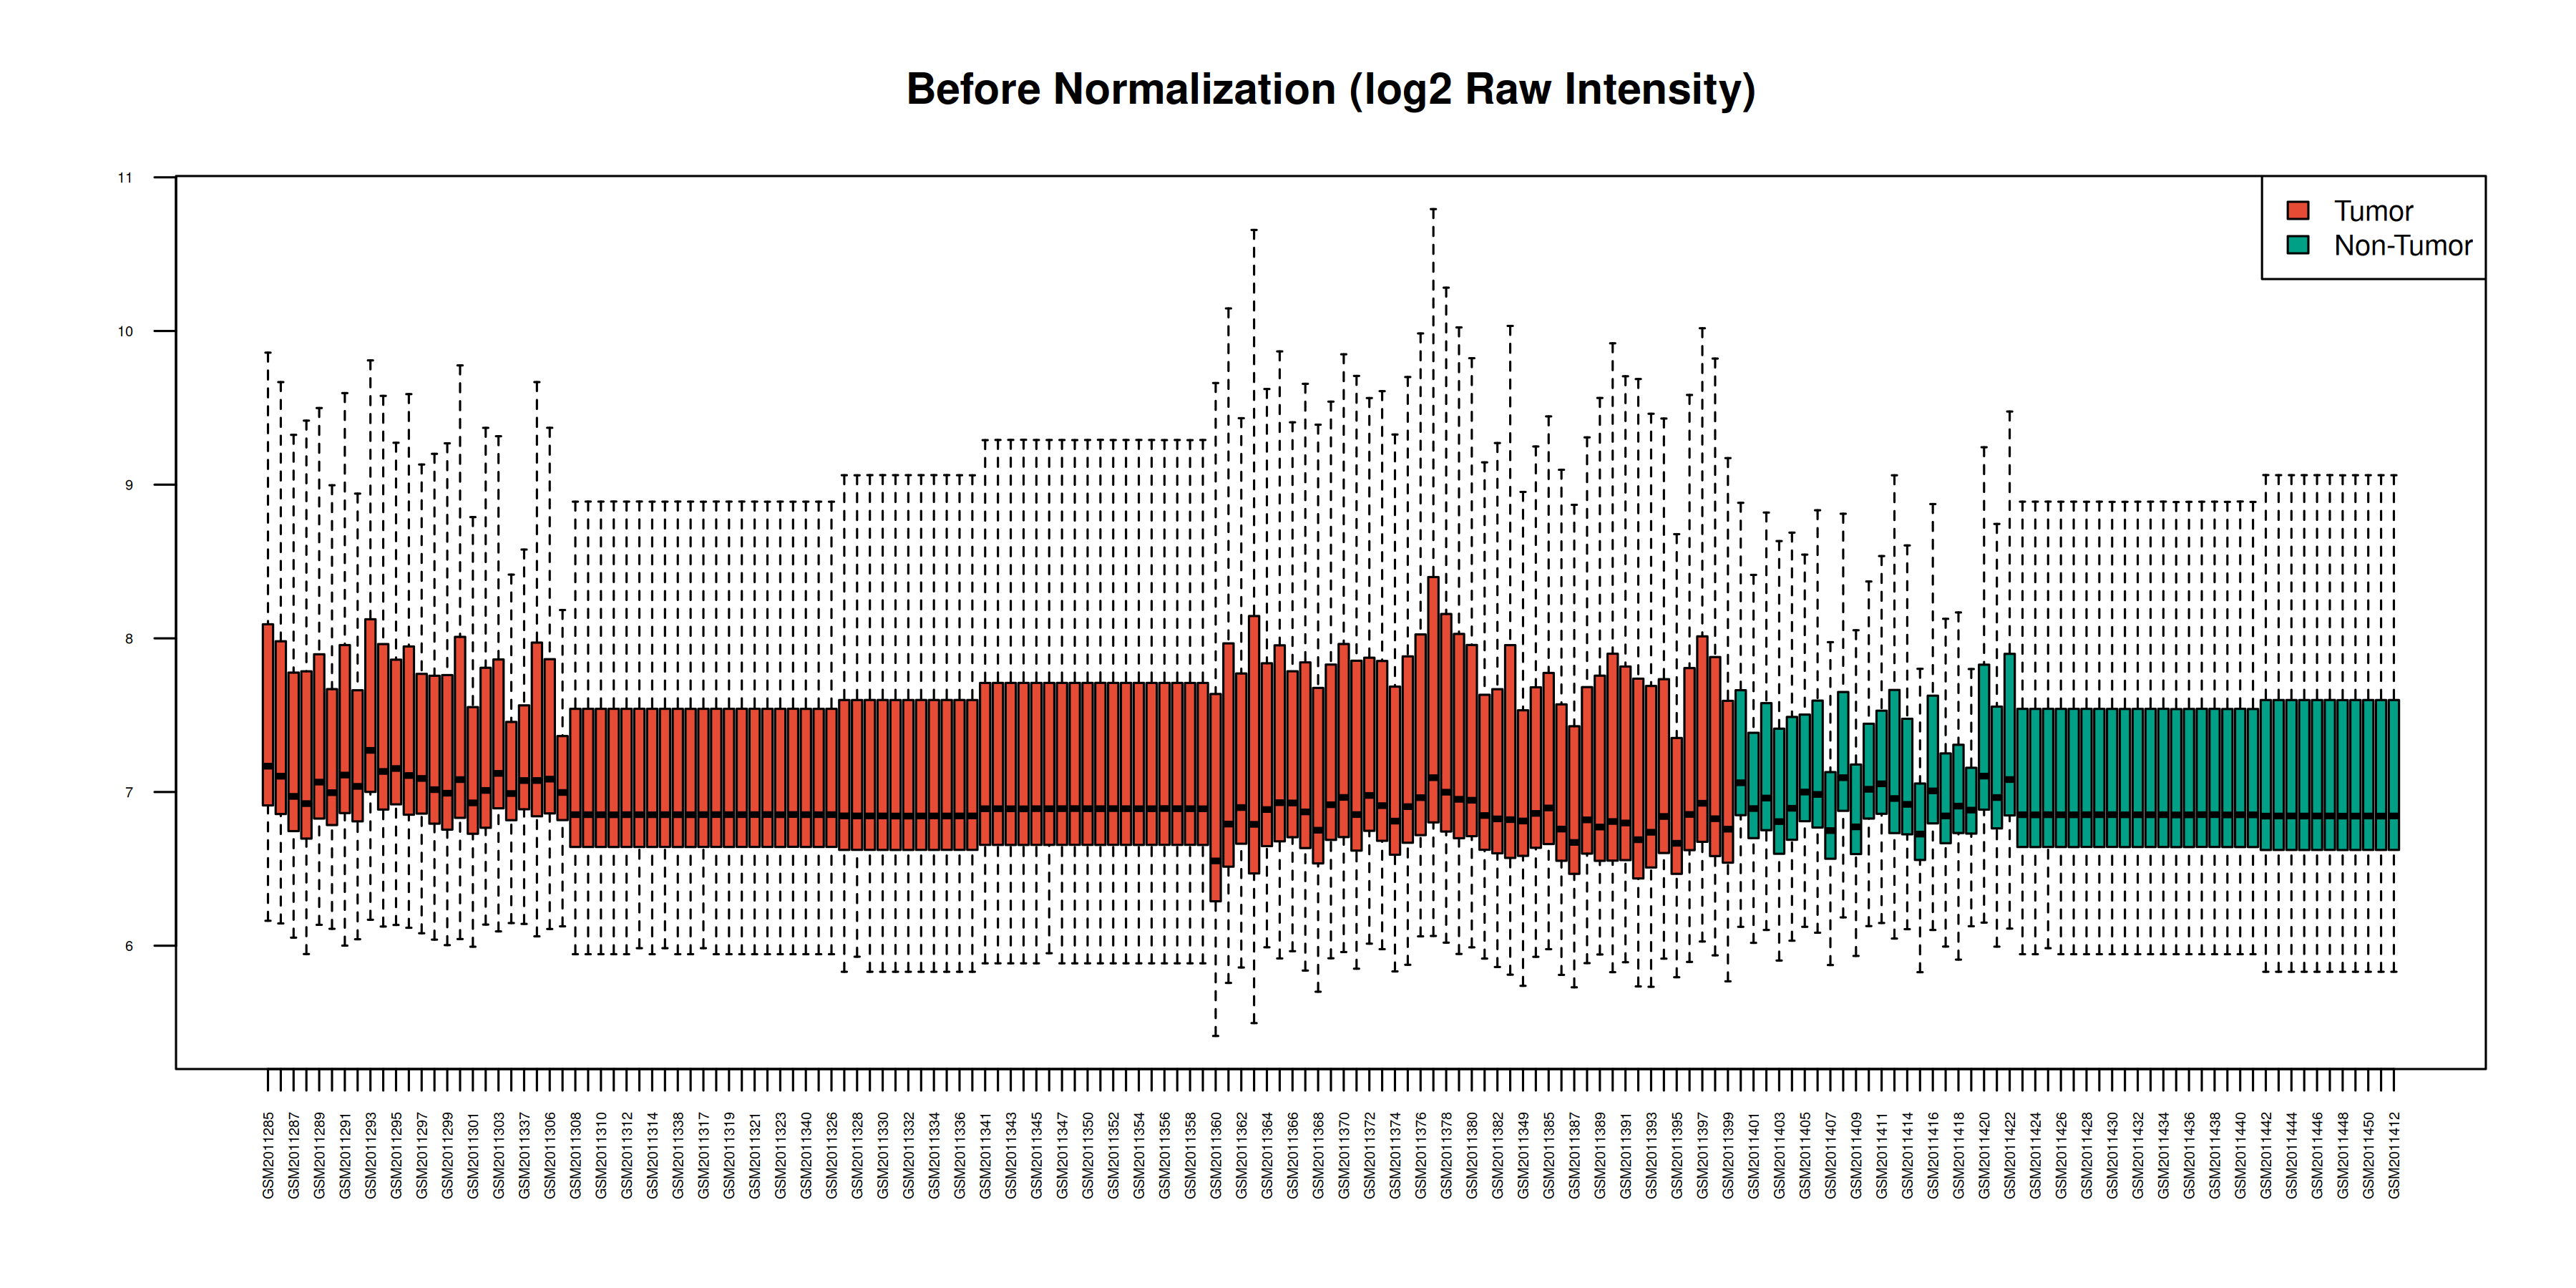
\includegraphics[width=\textwidth]{boxplot_before_norm.png}
\end{minipage}\hfill
\begin{minipage}{0.49\textwidth}
\centering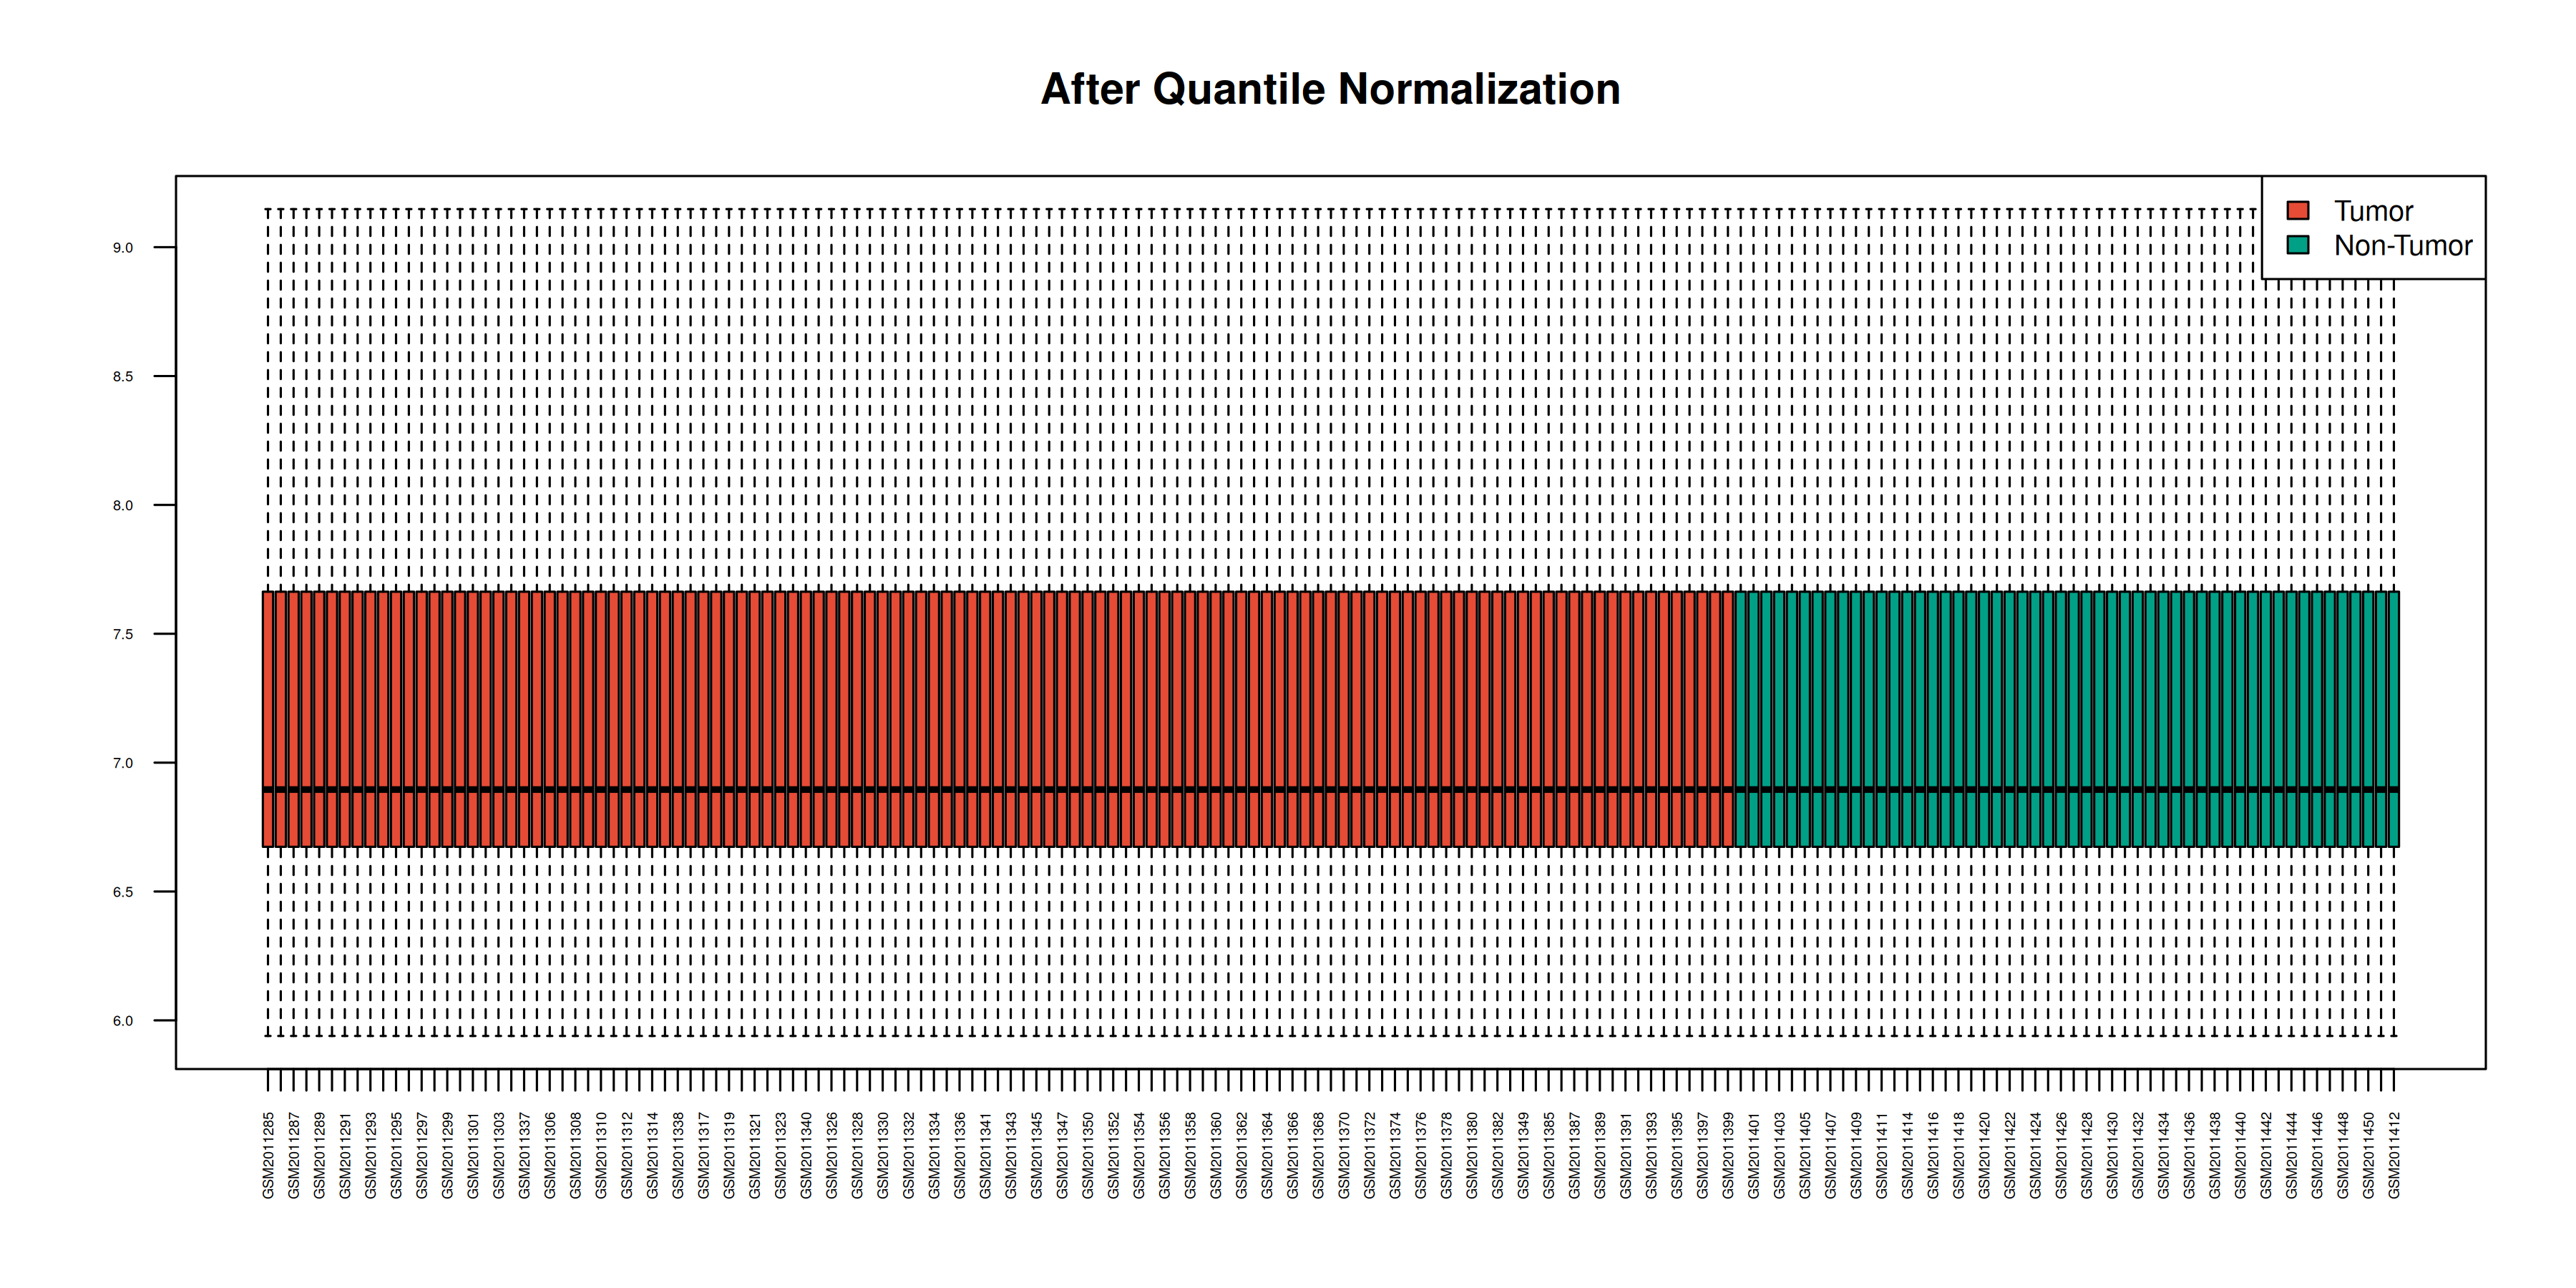
\includegraphics[width=\textwidth]{boxplot_after_norm.png}
\end{minipage}
\caption{Normalizasyon öncesi (sol) ve sonrası (sağ) örnek bazlı kutu grafikleri}
\label{fig:boxnorm}
\end{figure}

\begin{figure}[H]
\centering
\begin{minipage}{0.49\textwidth}
\centering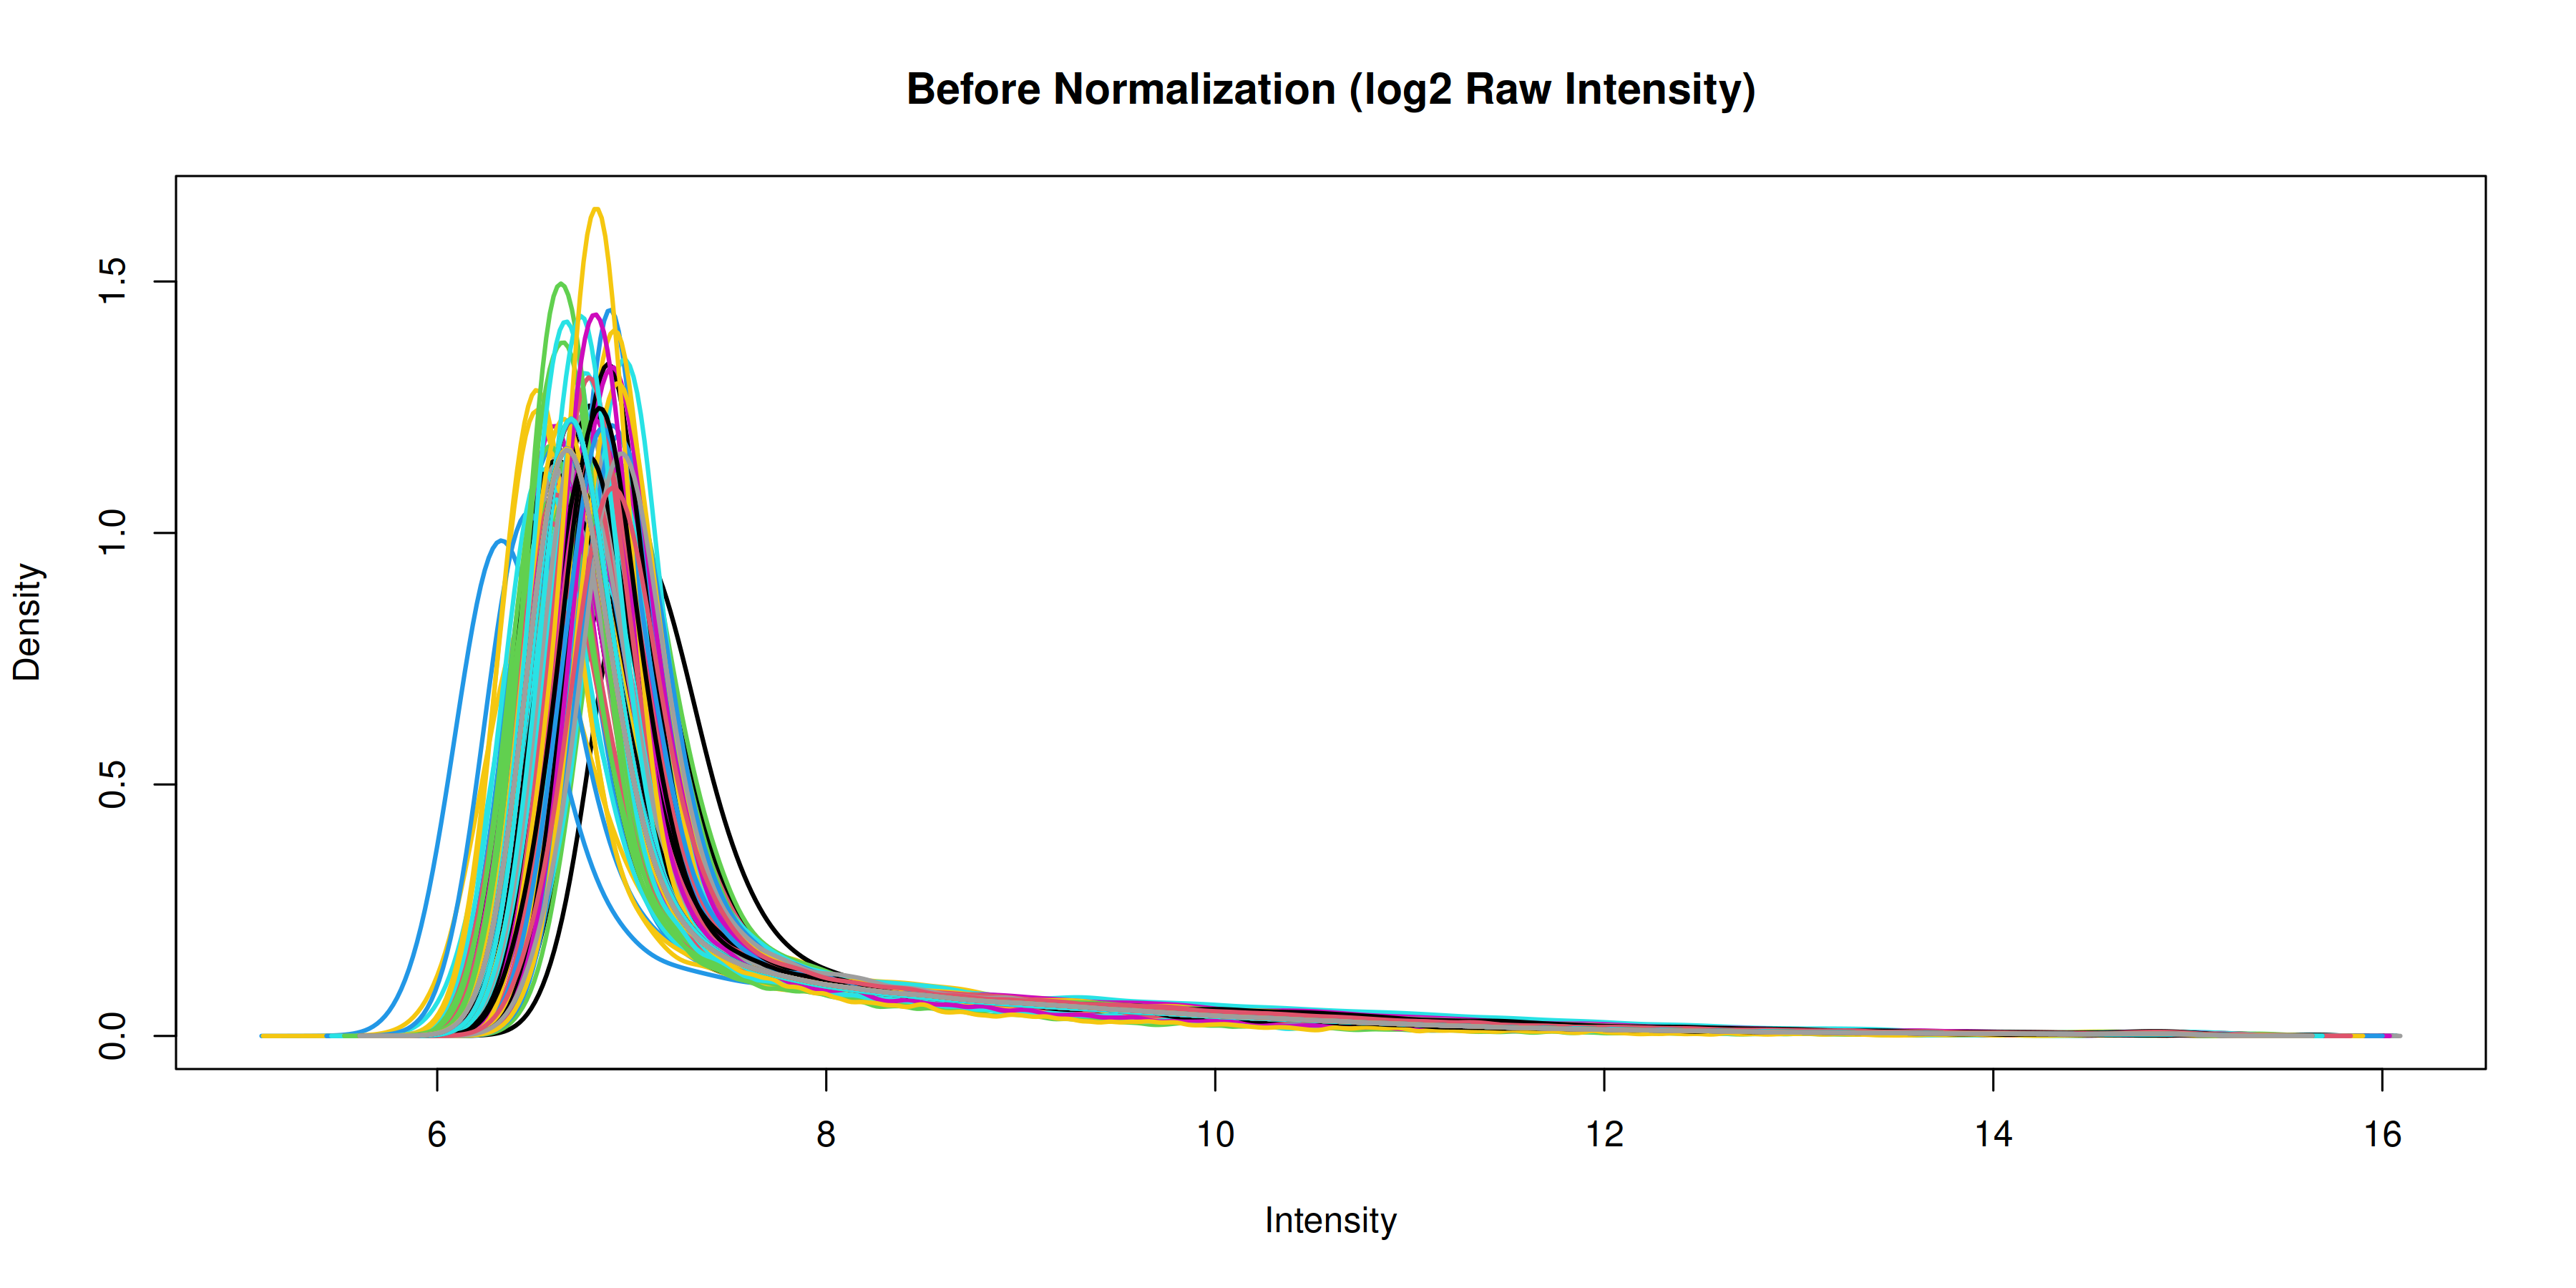
\includegraphics[width=\textwidth]{density_before_norm.png}
\end{minipage}\hfill
\begin{minipage}{0.49\textwidth}
\centering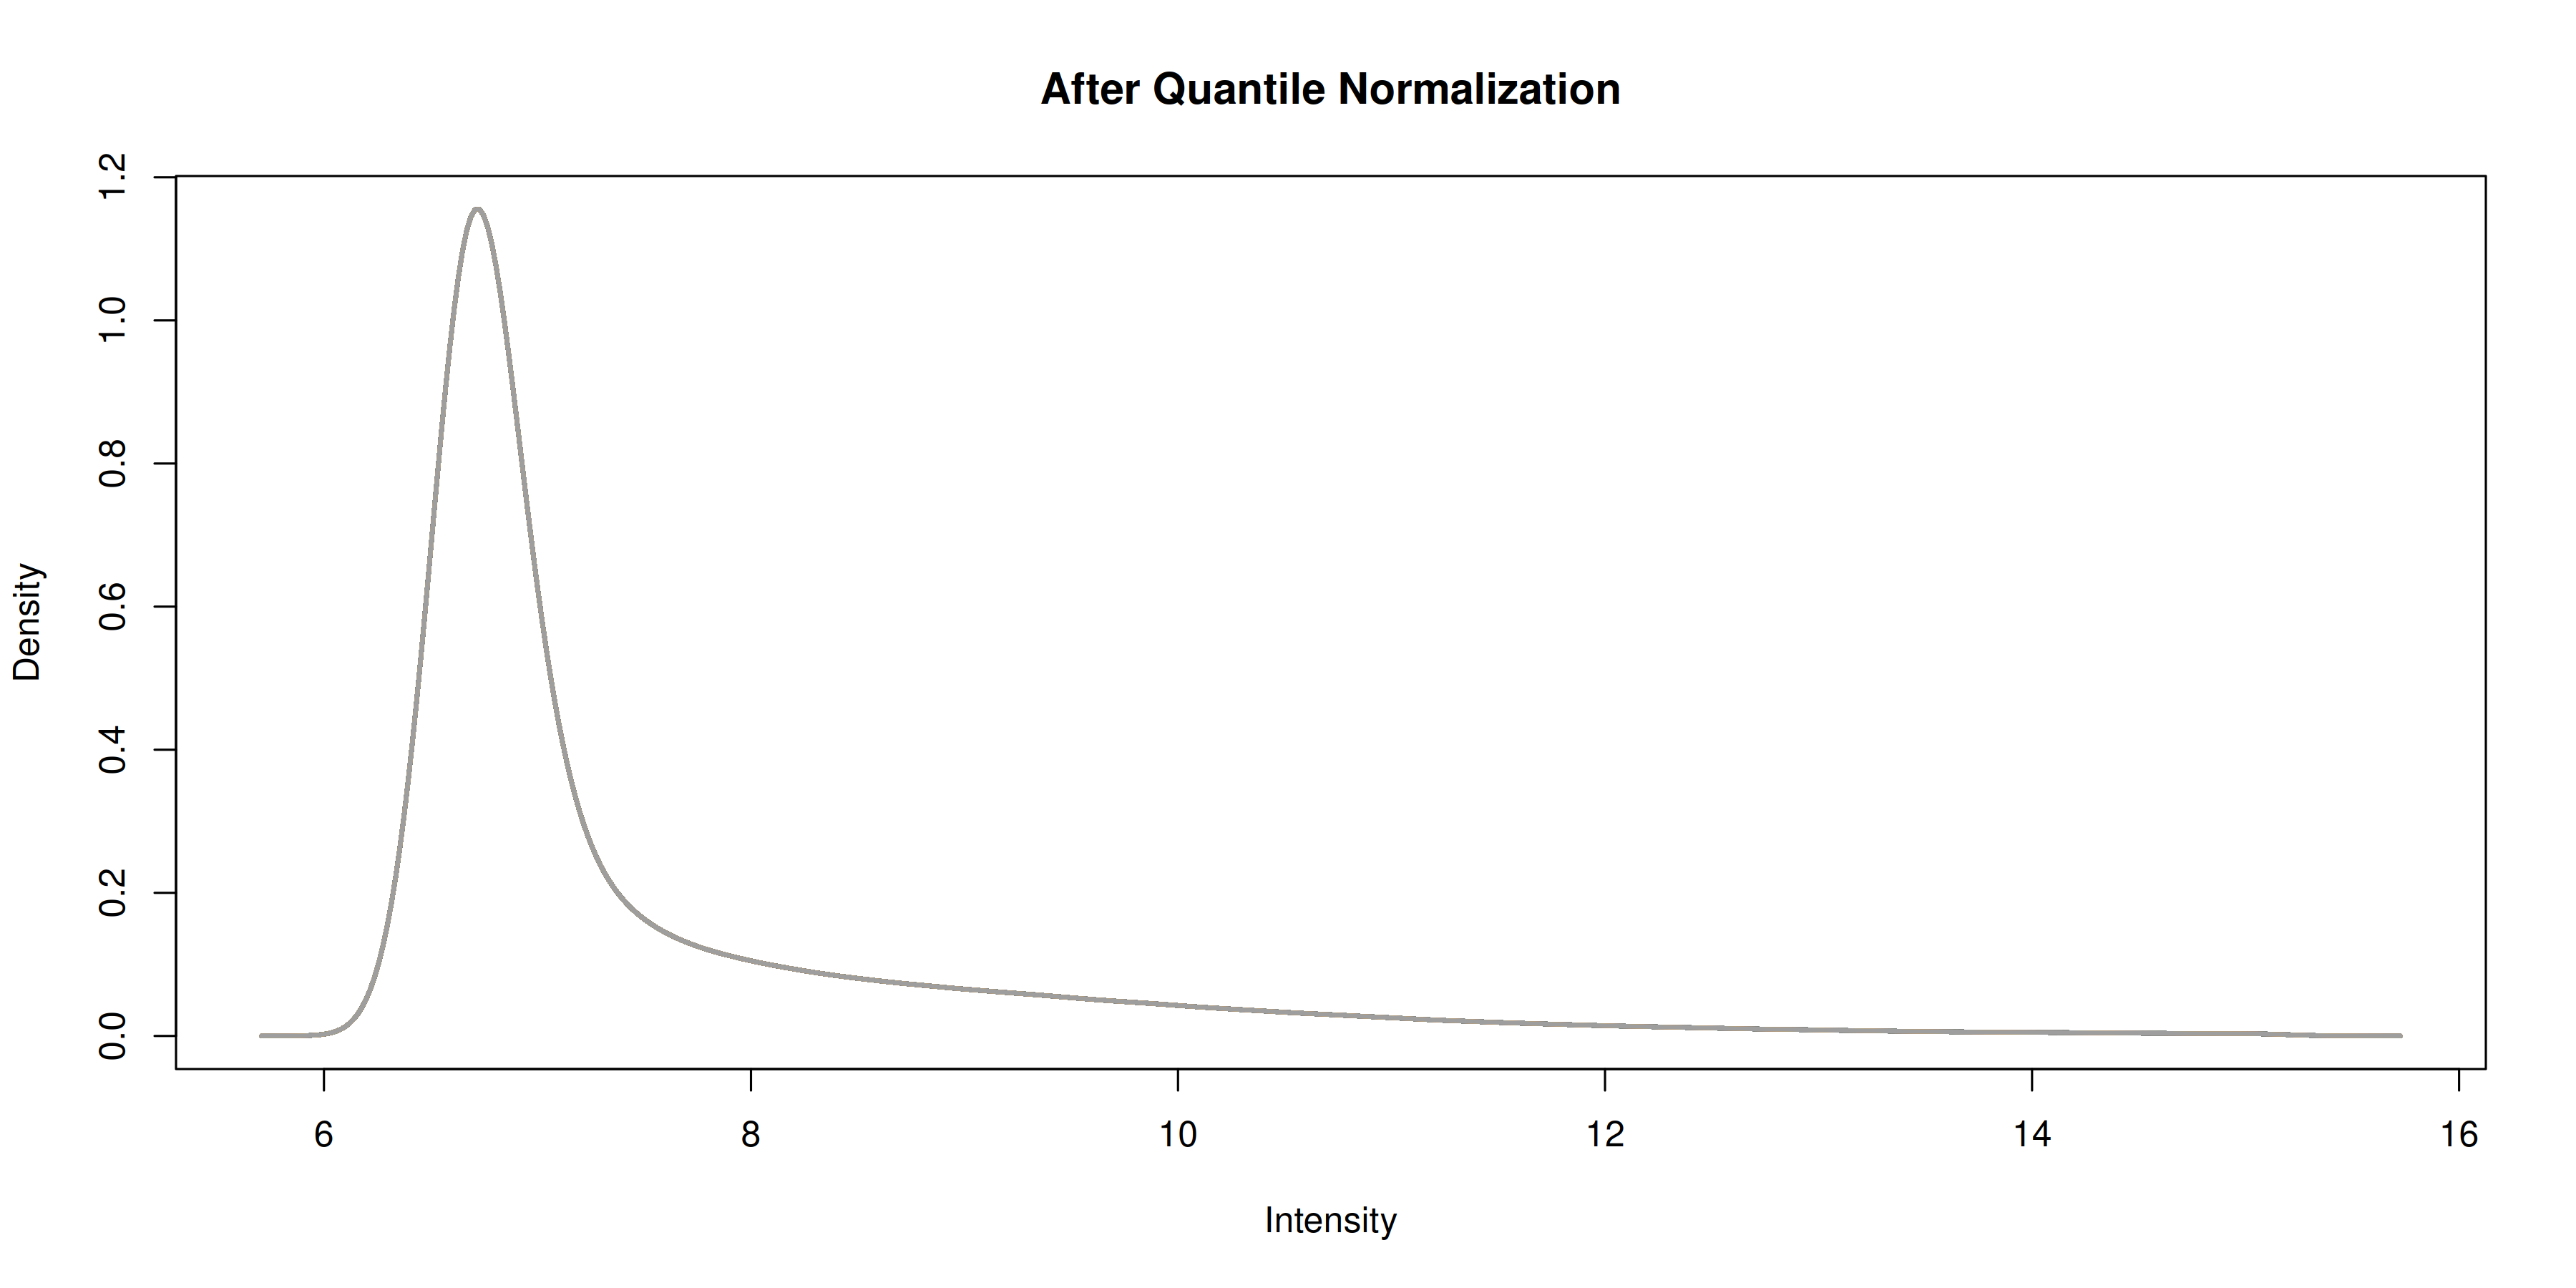
\includegraphics[width=\textwidth]{density_after_norm.png}
\end{minipage}
\caption{Normalizasyon öncesi (sol) ve sonrası (sağ) örnek bazlı yoğunluk dağılımları}
\label{fig:densnorm}
\end{figure}

\section{Prob Filtreleme ve Gen Anotasyonu}

Normalizasyon sonrasında veri setindeki düşük kaliteli ve bilgi değeri düşük problar çıkarılmıştır. Bu işlem üç adımda gerçekleştirilmiştir:

\begin{itemize}
    \item \textbf{Detection p-value filtresi:} Örneklerin en az \%10'unda güvenilir şekilde ölçülen problar tutulmuştur. Bu adım sonunda prob sayısı 47.322'den 27.050'ye düşmüştür.
    
    \item \textbf{Varyans filtresi:} İfade değerleri örnekler arasında çok az değişen problar analizden çıkarılmıştır. Bu amaçla en düşük \%10'luk varyansa sahip problar elenmiş ve prob sayısı 24.345'e düşmüştür.
    
    \item \textbf{Gen anotasyonu:} Probe ID'leri, GSE76427 veri setinin platform bilgisi kullanılarak gen sembollerine dönüştürülmüştür. Aynı gene karşılık gelen birden fazla prob olduğunda, en yüksek varyansa sahip prob seçilmiştir.
\end{itemize}

Bu adımlar sonucunda analiz için 14.323 benzersiz gen elde edilmiştir.


\section{Yüksek Varyanslı Gen (HVG) Seçimi}

Filtreleme ve anotasyon adımlarından sonra genler, örnekler arasındaki değişkenlik düzeylerine göre sıralanmıştır. En yüksek varyansa sahip 3000 gen seçilerek HVG listesi oluşturulmuştur.

Bu adımın amacı, örnekler arasında çok az değişen ve analizlere sınırlı katkı sağlayan genleri dışarıda bırakmaktır. Böylece PCA, WGCNA ve makine öğrenmesi analizlerinde daha bilgilendirici genlerle çalışılmıştır.


\section{Keşifsel Veri Analizi}

HVG seçimi öncesi ve sonrası temel bileşen analizi (PCA) Şekil~\ref{fig:pca} ile verilmiştir. Sınıflara göre renklendirilmiş PCA grafiğinde (Şekil~\ref{fig:pcagroup}) tümör ve non-tümör örnekleri belirgin biçimde ayrışmaktadır. En yüksek varyansa sahip 20 gene ait ısı haritası (Şekil~\ref{fig:heatmaphvg}) iki doku tipinin ayrı kümeler oluşturduğunu göstermektedir.

\begin{figure}[H]
\centering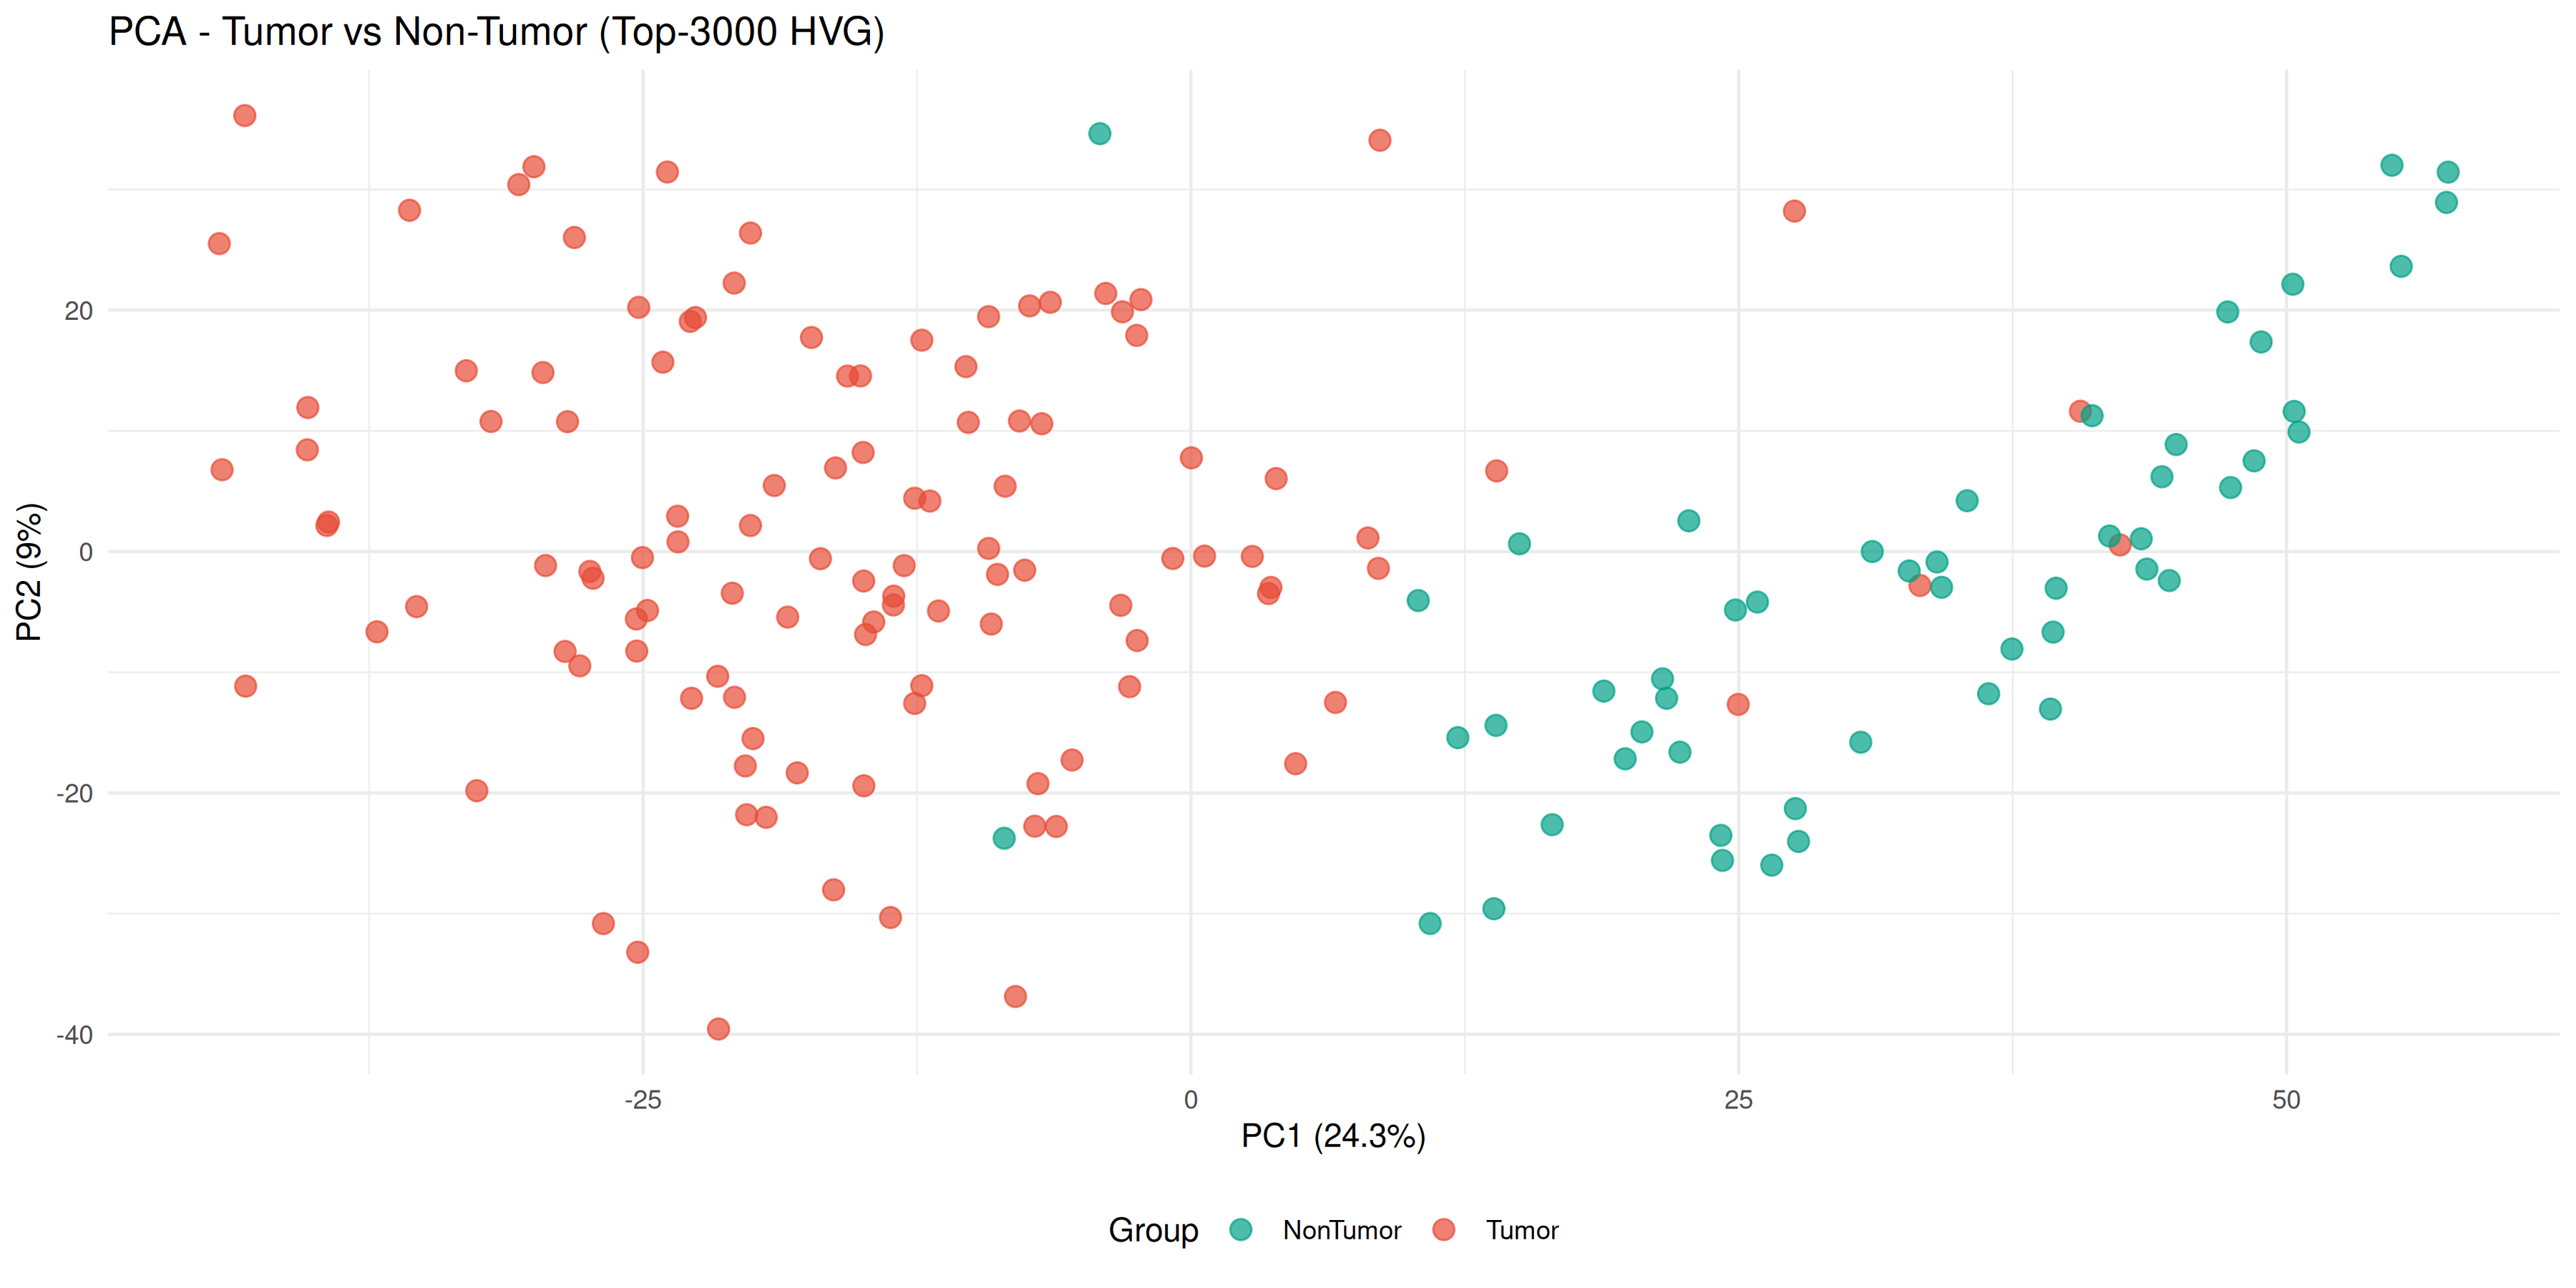
\includegraphics[width=0.95\textwidth]{pca_colored_by_group.png}
\caption{Top-3000 HVG ile gruplara göre renklendirilmiş PCA grafiği}
\label{fig:pcagroup}
\end{figure}

\begin{figure}[H]
\centering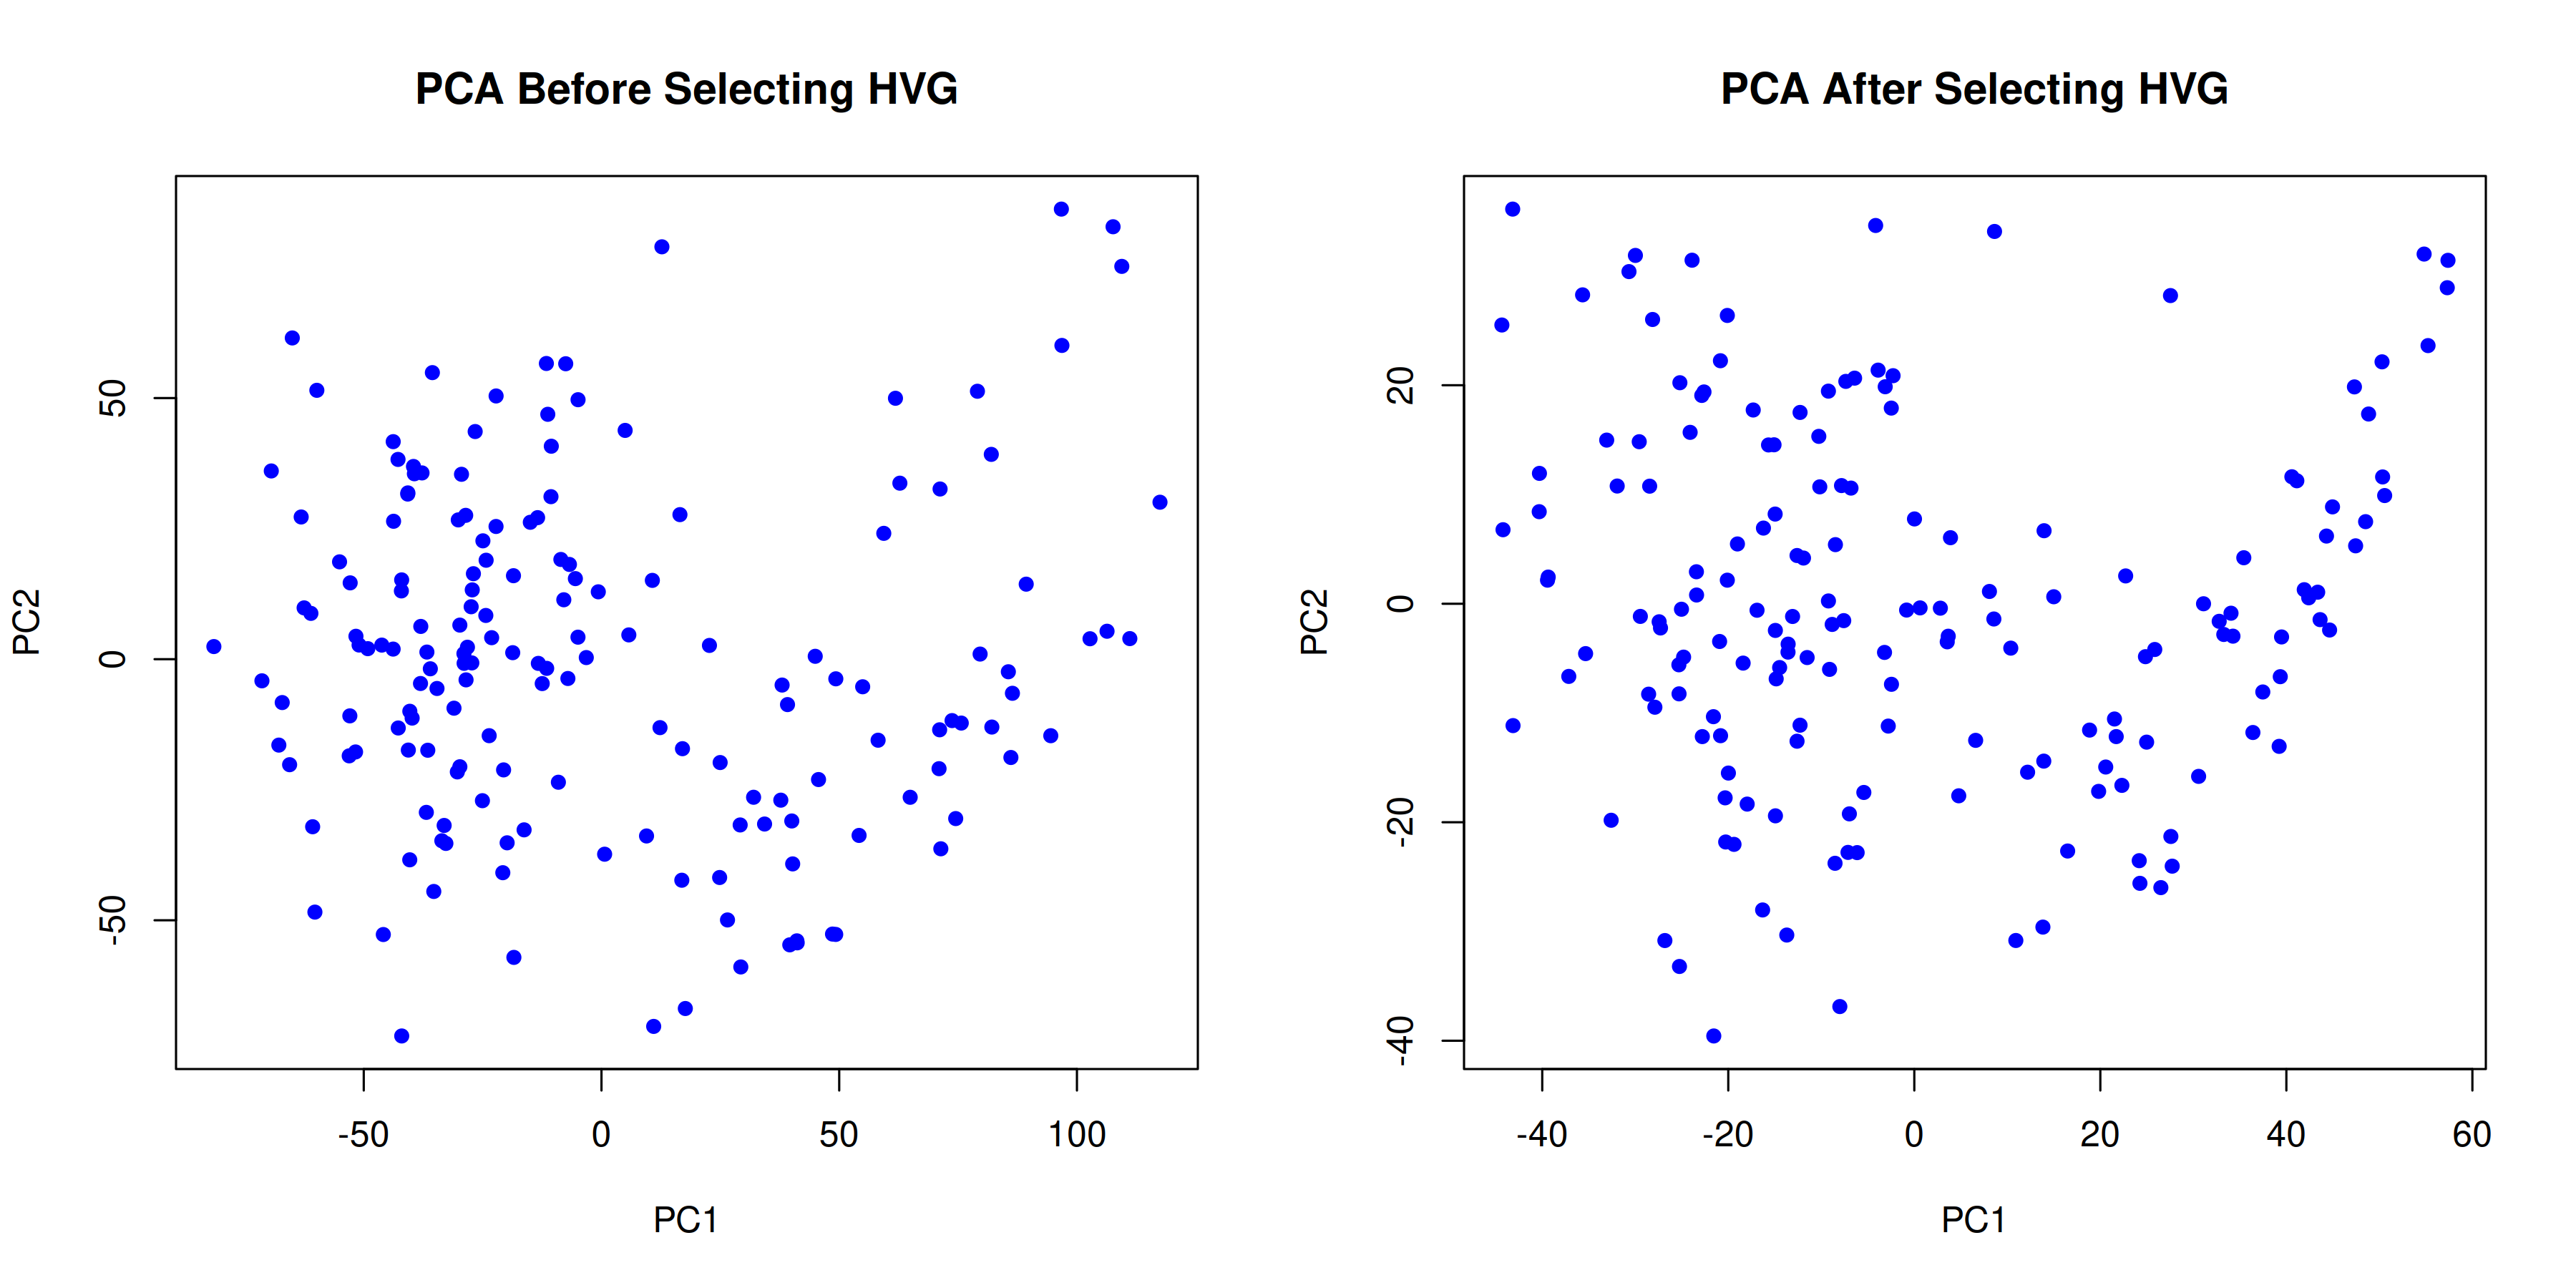
\includegraphics[width=0.9\textwidth]{pca_before_after_hvg.png}
\caption{HVG seçimi öncesi (sol) ve sonrası (sağ) PCA dağılımları}
\label{fig:pca}
\end{figure}

\begin{figure}[H]
\centering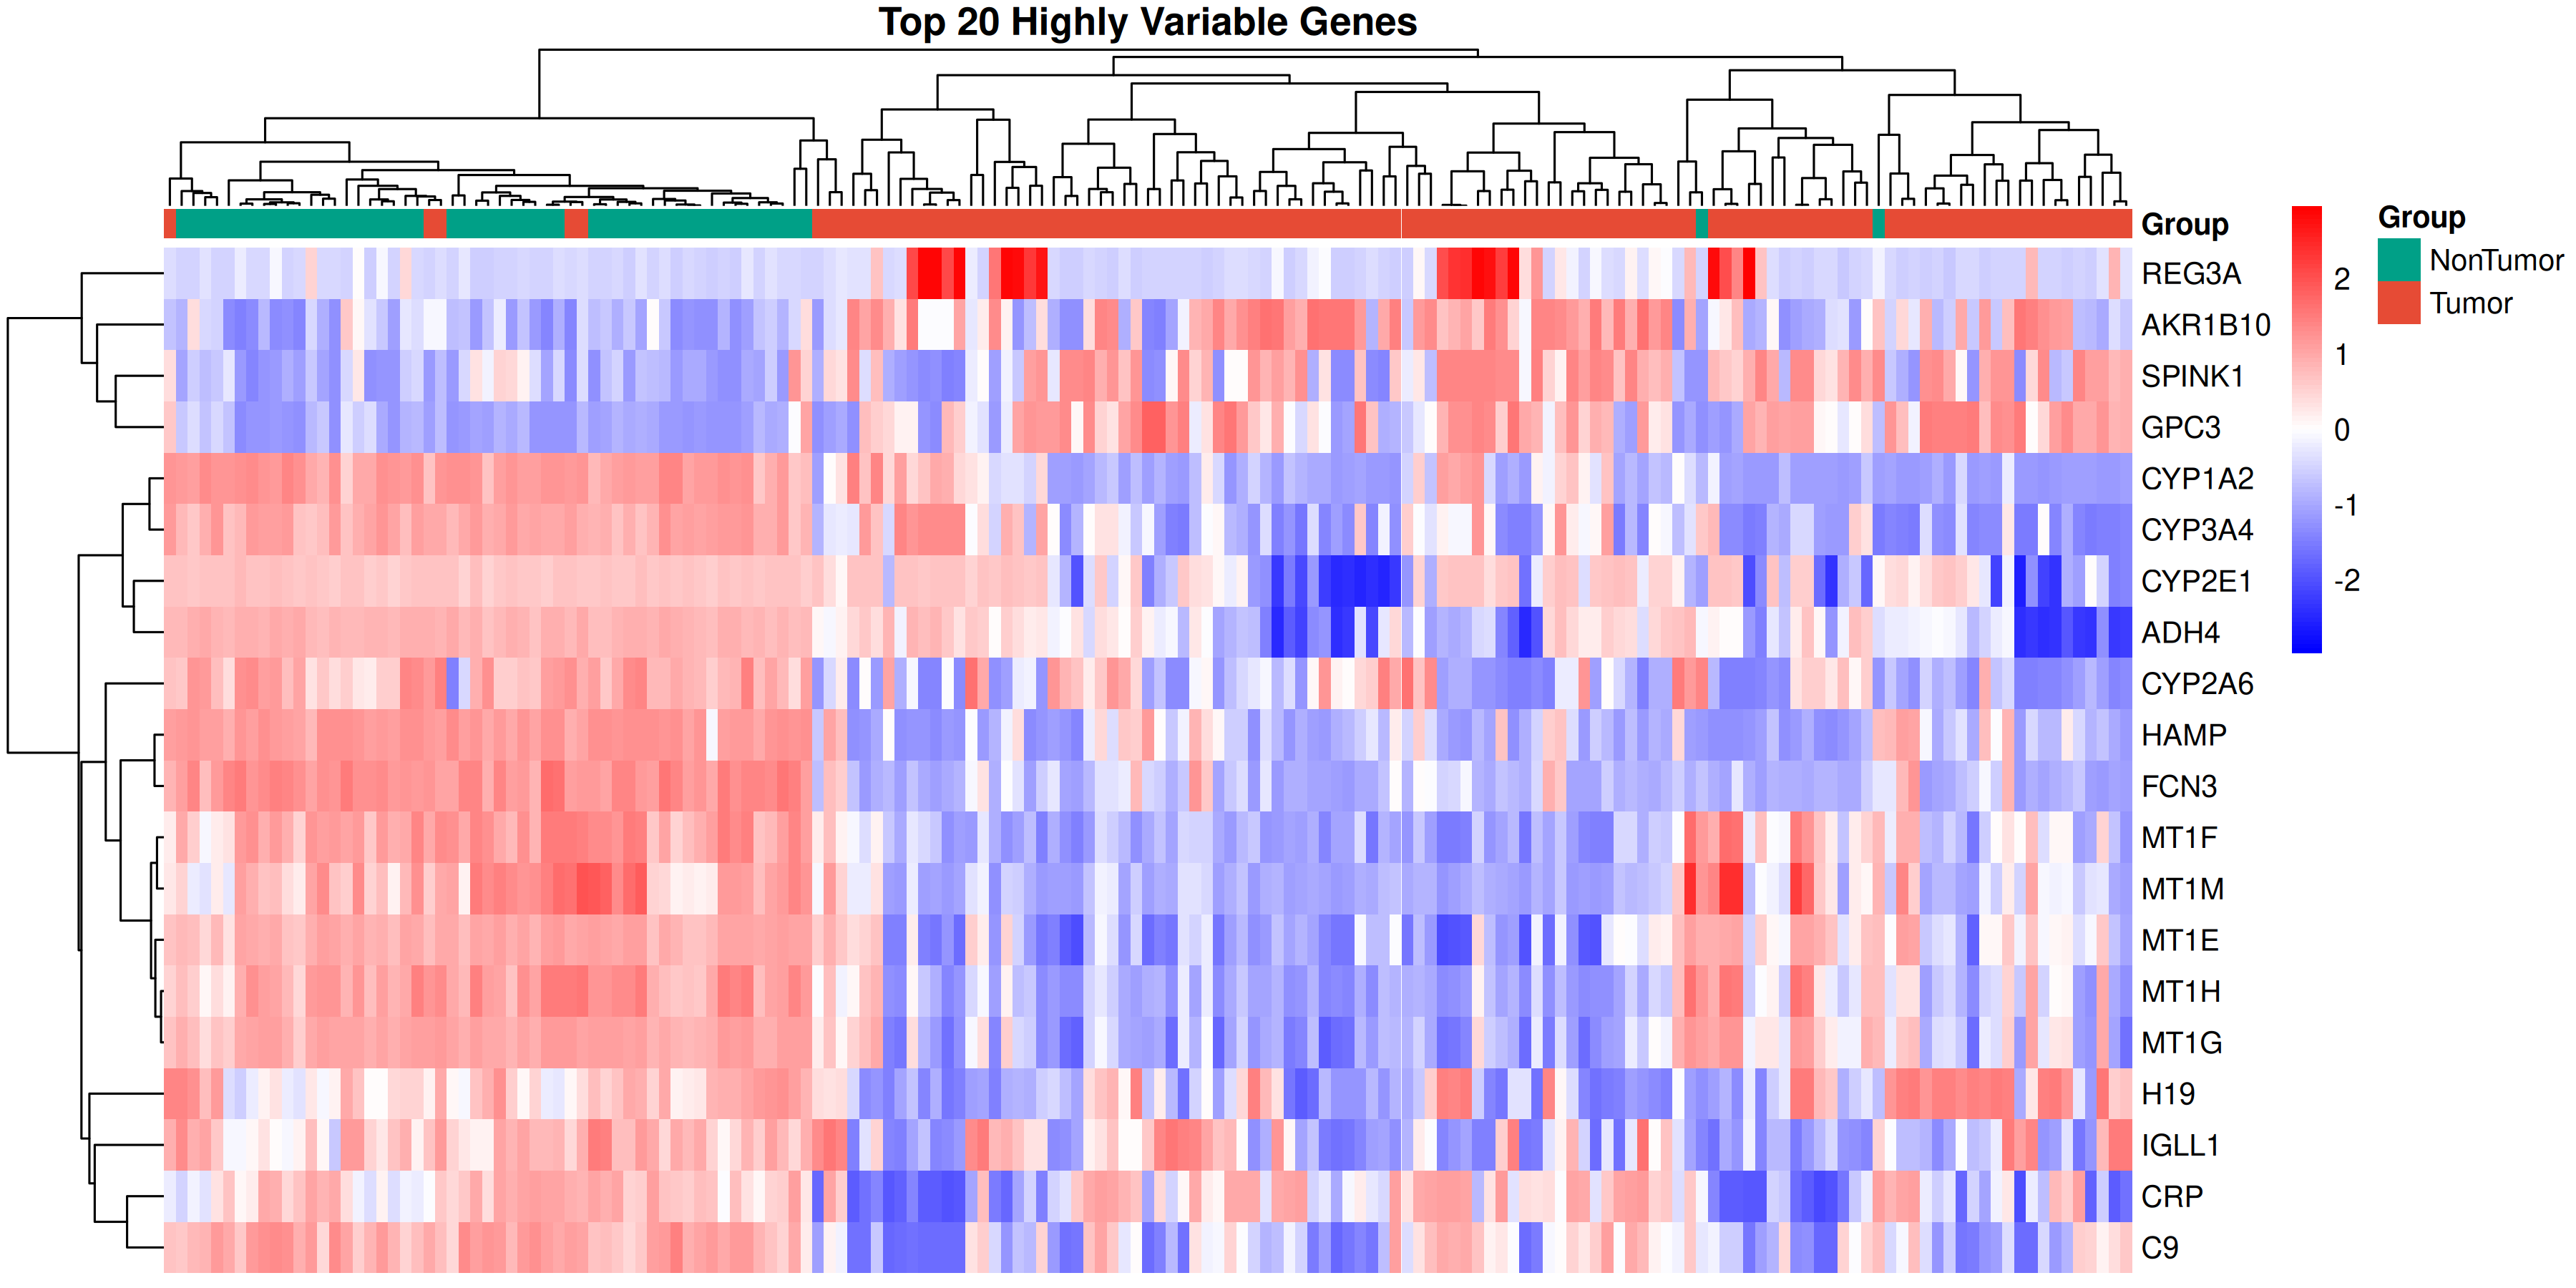
\includegraphics[width=0.95\textwidth]{heatmap_top20_hvg.png}
\caption{En yüksek varyansa sahip 20 genin grup anotasyonlu ısı haritası}
\label{fig:heatmaphvg}
\end{figure}

% ------------------------------------------------------------------------------
\chapter{DİFERANSİYEL GEN İFADESİ ANALİZİ}

\section{Yöntem}

Diferansiyel gen ifadesi (DGE) analizi, prob filtreleme ve gen anotasyonu sonrası elde edilen 14.323 benzersiz gen üzerinde gerçekleştirilmiştir. HVG seçimi bu aşamada kullanılmamış, yalnızca PCA, WGCNA ve makine öğrenmesi analizleri için uygulanmıştır.

Veri setinde bazı hastalara ait hem tümör hem de komşu non-tümör örnekleri bulunduğu için eşleşmiş örnek yapısı dikkate alınmıştır. Bu amaçla hasta kimliği modele eklenmiş ve tümör ile non-tümör dokular arasındaki gen ifade farkları karşılaştırılmıştır.

Analizde \texttt{limma} paketi kullanılmıştır. Tümör ve non-tümör grupları için uygun tasarım matrisi tanımlanmıştır. Daha sonra model kurulmuş ve her gen için istatistiksel anlamlılık değerleri hesaplanmıştır.


Anlamlı genler, düzeltilmiş p-değeri \textbf{0,05'ten küçük} ve mutlak logFC değeri \textbf{1'den büyük} olacak şekilde seçilmiştir. Bu eşikler, hem istatistiksel anlamlılığı hem de ifade değişiminin büyüklüğünü birlikte değerlendirmek için kullanılmıştır.

\section{Sonuçlar}

Analiz sonucunda 705 genin tümör ve non-tümör örnekleri arasında anlamlı düzeyde farklı ifade edildiği belirlenmiştir: 216 up-regulated ve 489 down-regulated. Down-regulated genlerin baskınlığı, HCC dokusunda hepatositlere özgü bazı normal karaciğer fonksiyonlarının azalmış olabileceğini düşündürmektedir. En güçlü DEG'ler Tablo~\ref{tab:deg} içinde verilmiştir.

\begin{table}[H]
\centering
\caption{En güçlü diferansiyel ifadeli genler}
\label{tab:deg}
\begin{tabular}{llrl}
\toprule
\textbf{Gen} & \textbf{Yön} & \textbf{logFC} & \textbf{adj.P.Val} \\
\midrule
GPC3     & Up   & $+3{,}53$ & $5{,}91\times10^{-20}$ \\
AKR1B10  & Up   & $+3{,}06$ & $6{,}28\times10^{-13}$ \\
SPINK1   & Up   & $+2{,}89$ & $1{,}39\times10^{-9}$ \\
TOP2A    & Up   & $+2{,}58$ & $1{,}04\times10^{-28}$ \\
ACSL4    & Up   & $+2{,}53$ & $1{,}07\times10^{-17}$ \\
\midrule
HAMP     & Down & $-5{,}00$ & $2{,}08\times10^{-29}$ \\
CYP1A2   & Down & $-4{,}75$ & $1{,}49\times10^{-25}$ \\
FCN3     & Down & $-4{,}64$ & $2{,}11\times10^{-39}$ \\
MT1H     & Down & $-4{,}21$ & $3{,}29\times10^{-25}$ \\
MT1G     & Down & $-4{,}04$ & $4{,}16\times10^{-23}$ \\
\bottomrule
\end{tabular}
\end{table}

\section{Görselleştirmeler}

DGE sonuçları volkan grafiği (Şekil~\ref{fig:volcano}), kutu grafikleri (Şekil~\ref{fig:boxtop5}), keman grafikleri (Şekil~\ref{fig:violin}) ve ısı haritası (Şekil~\ref{fig:heatmapdeg}) ile gösterilmiştir. Kutu ve keman grafikleri, mutlak logFC değerine göre seçilen en güçlü 5 gen için hazırlanmıştır. Bu beş genin tamamı down-regulated olduğu için, survival analizinde ayrıca en güçlü 5 up-regulated gen de değerlendirilmiştir.

\begin{figure}[H]
\centering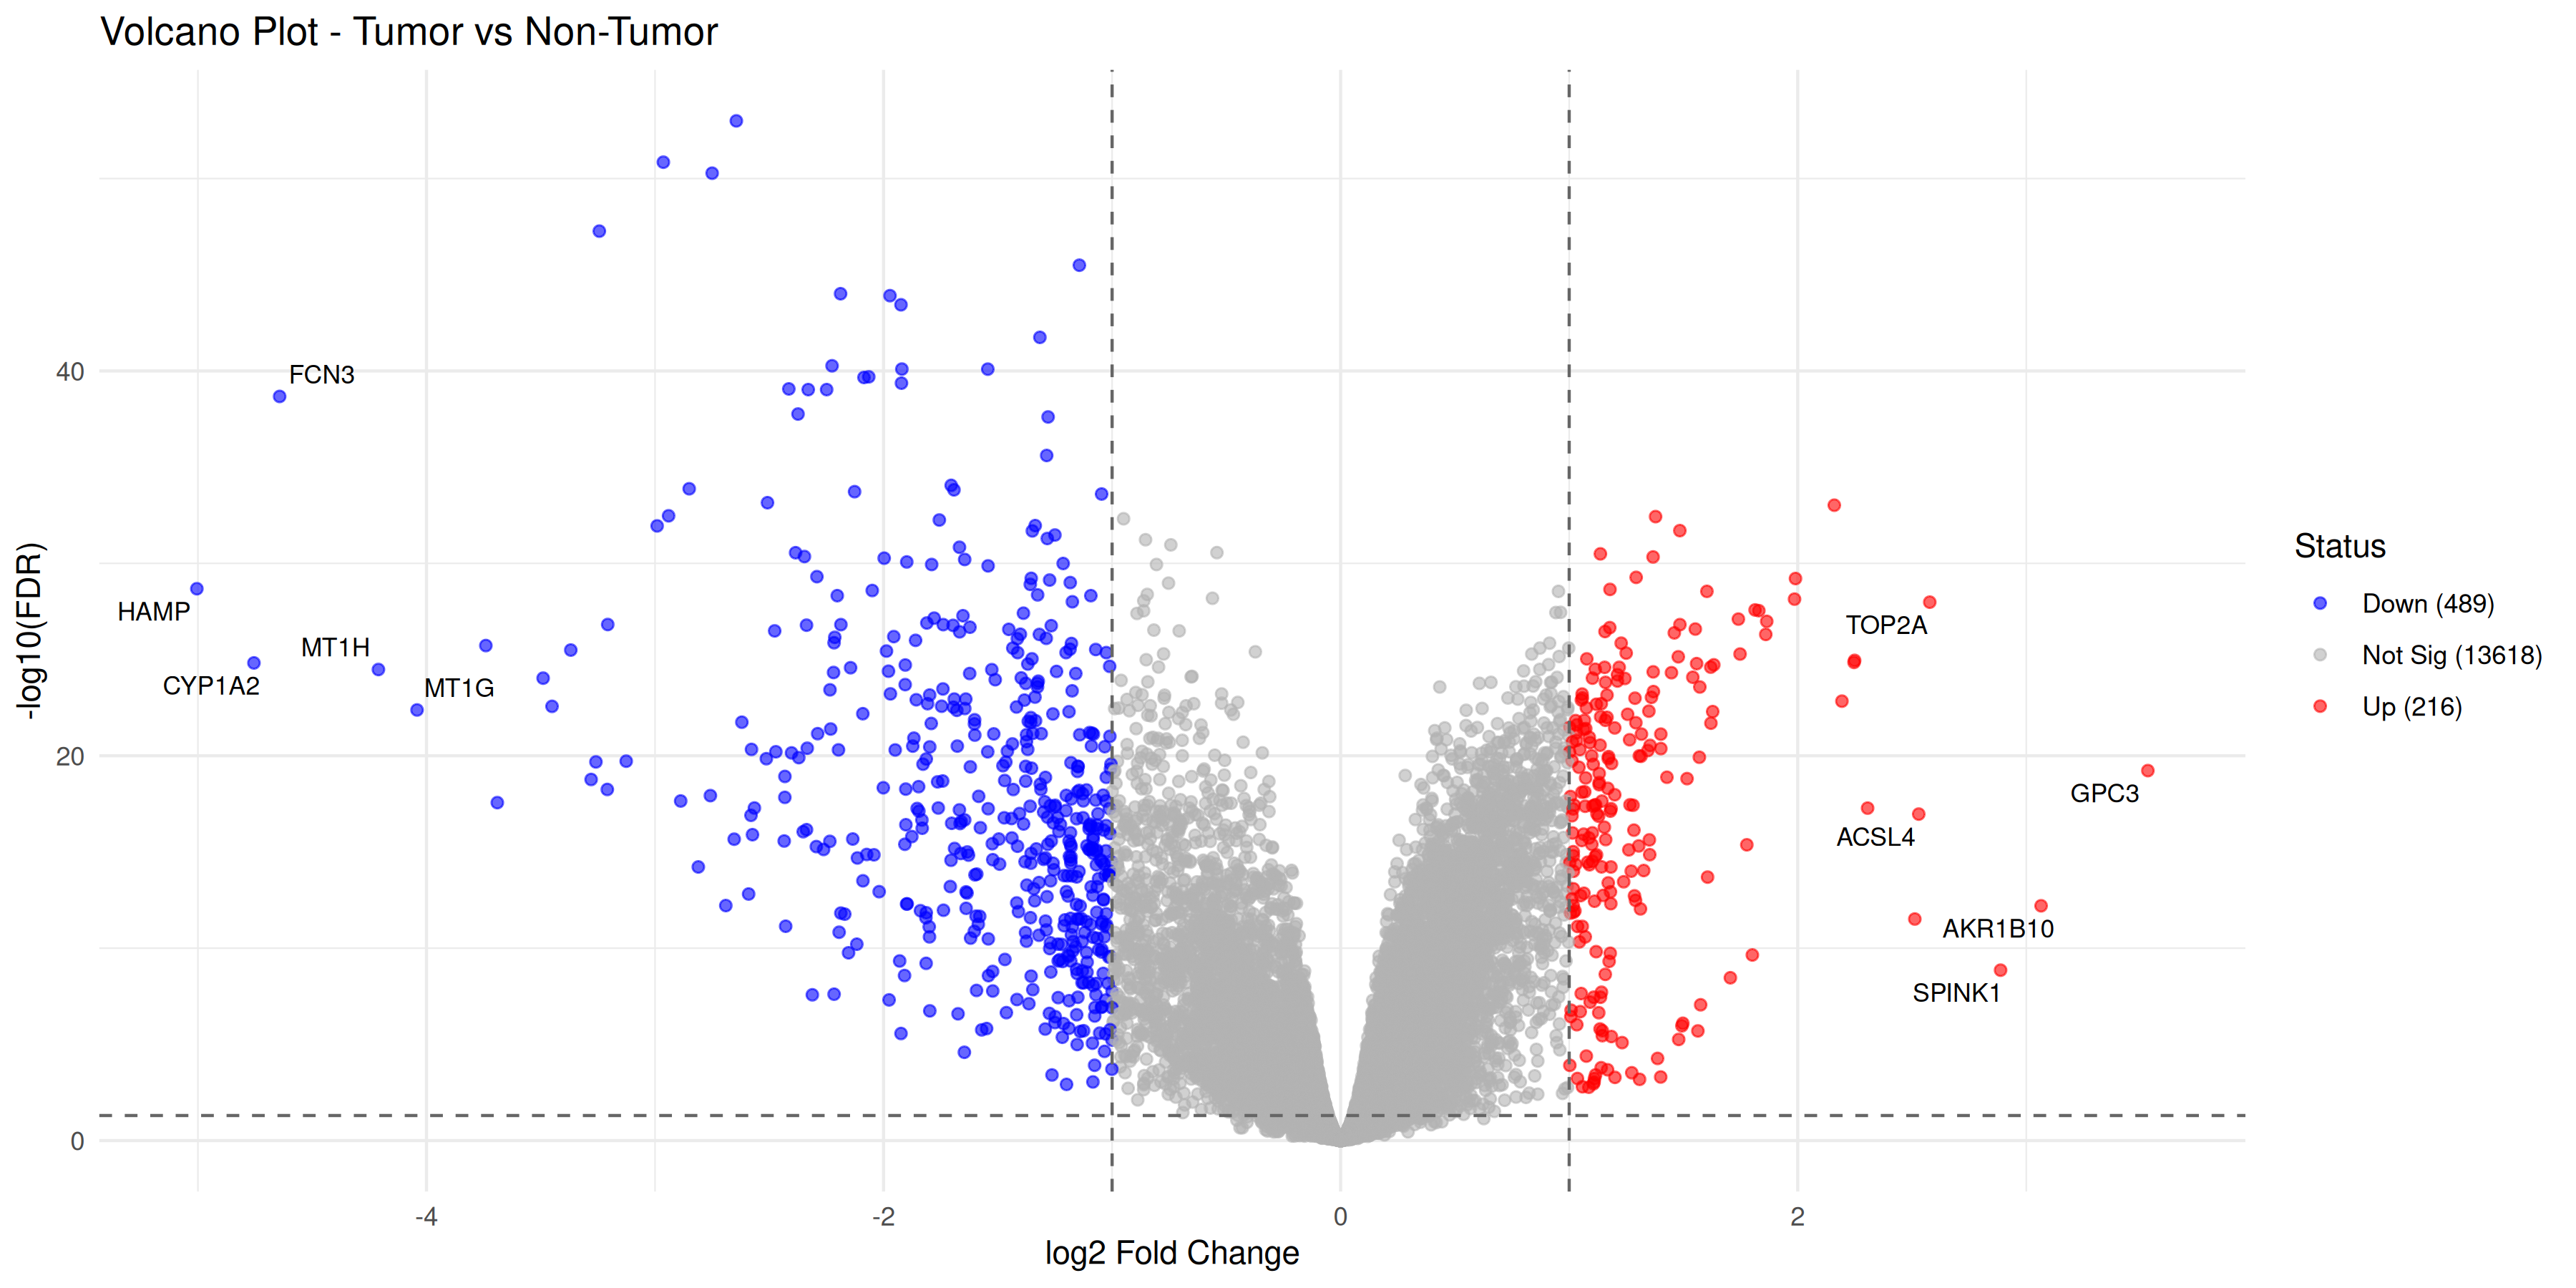
\includegraphics[width=0.95\textwidth]{volcano_plot.png}
\caption{Diferansiyel gen ifadesi volkan grafiği (kırmızı: up, mavi: down)}
\label{fig:volcano}
\end{figure}

\begin{figure}[H]
\centering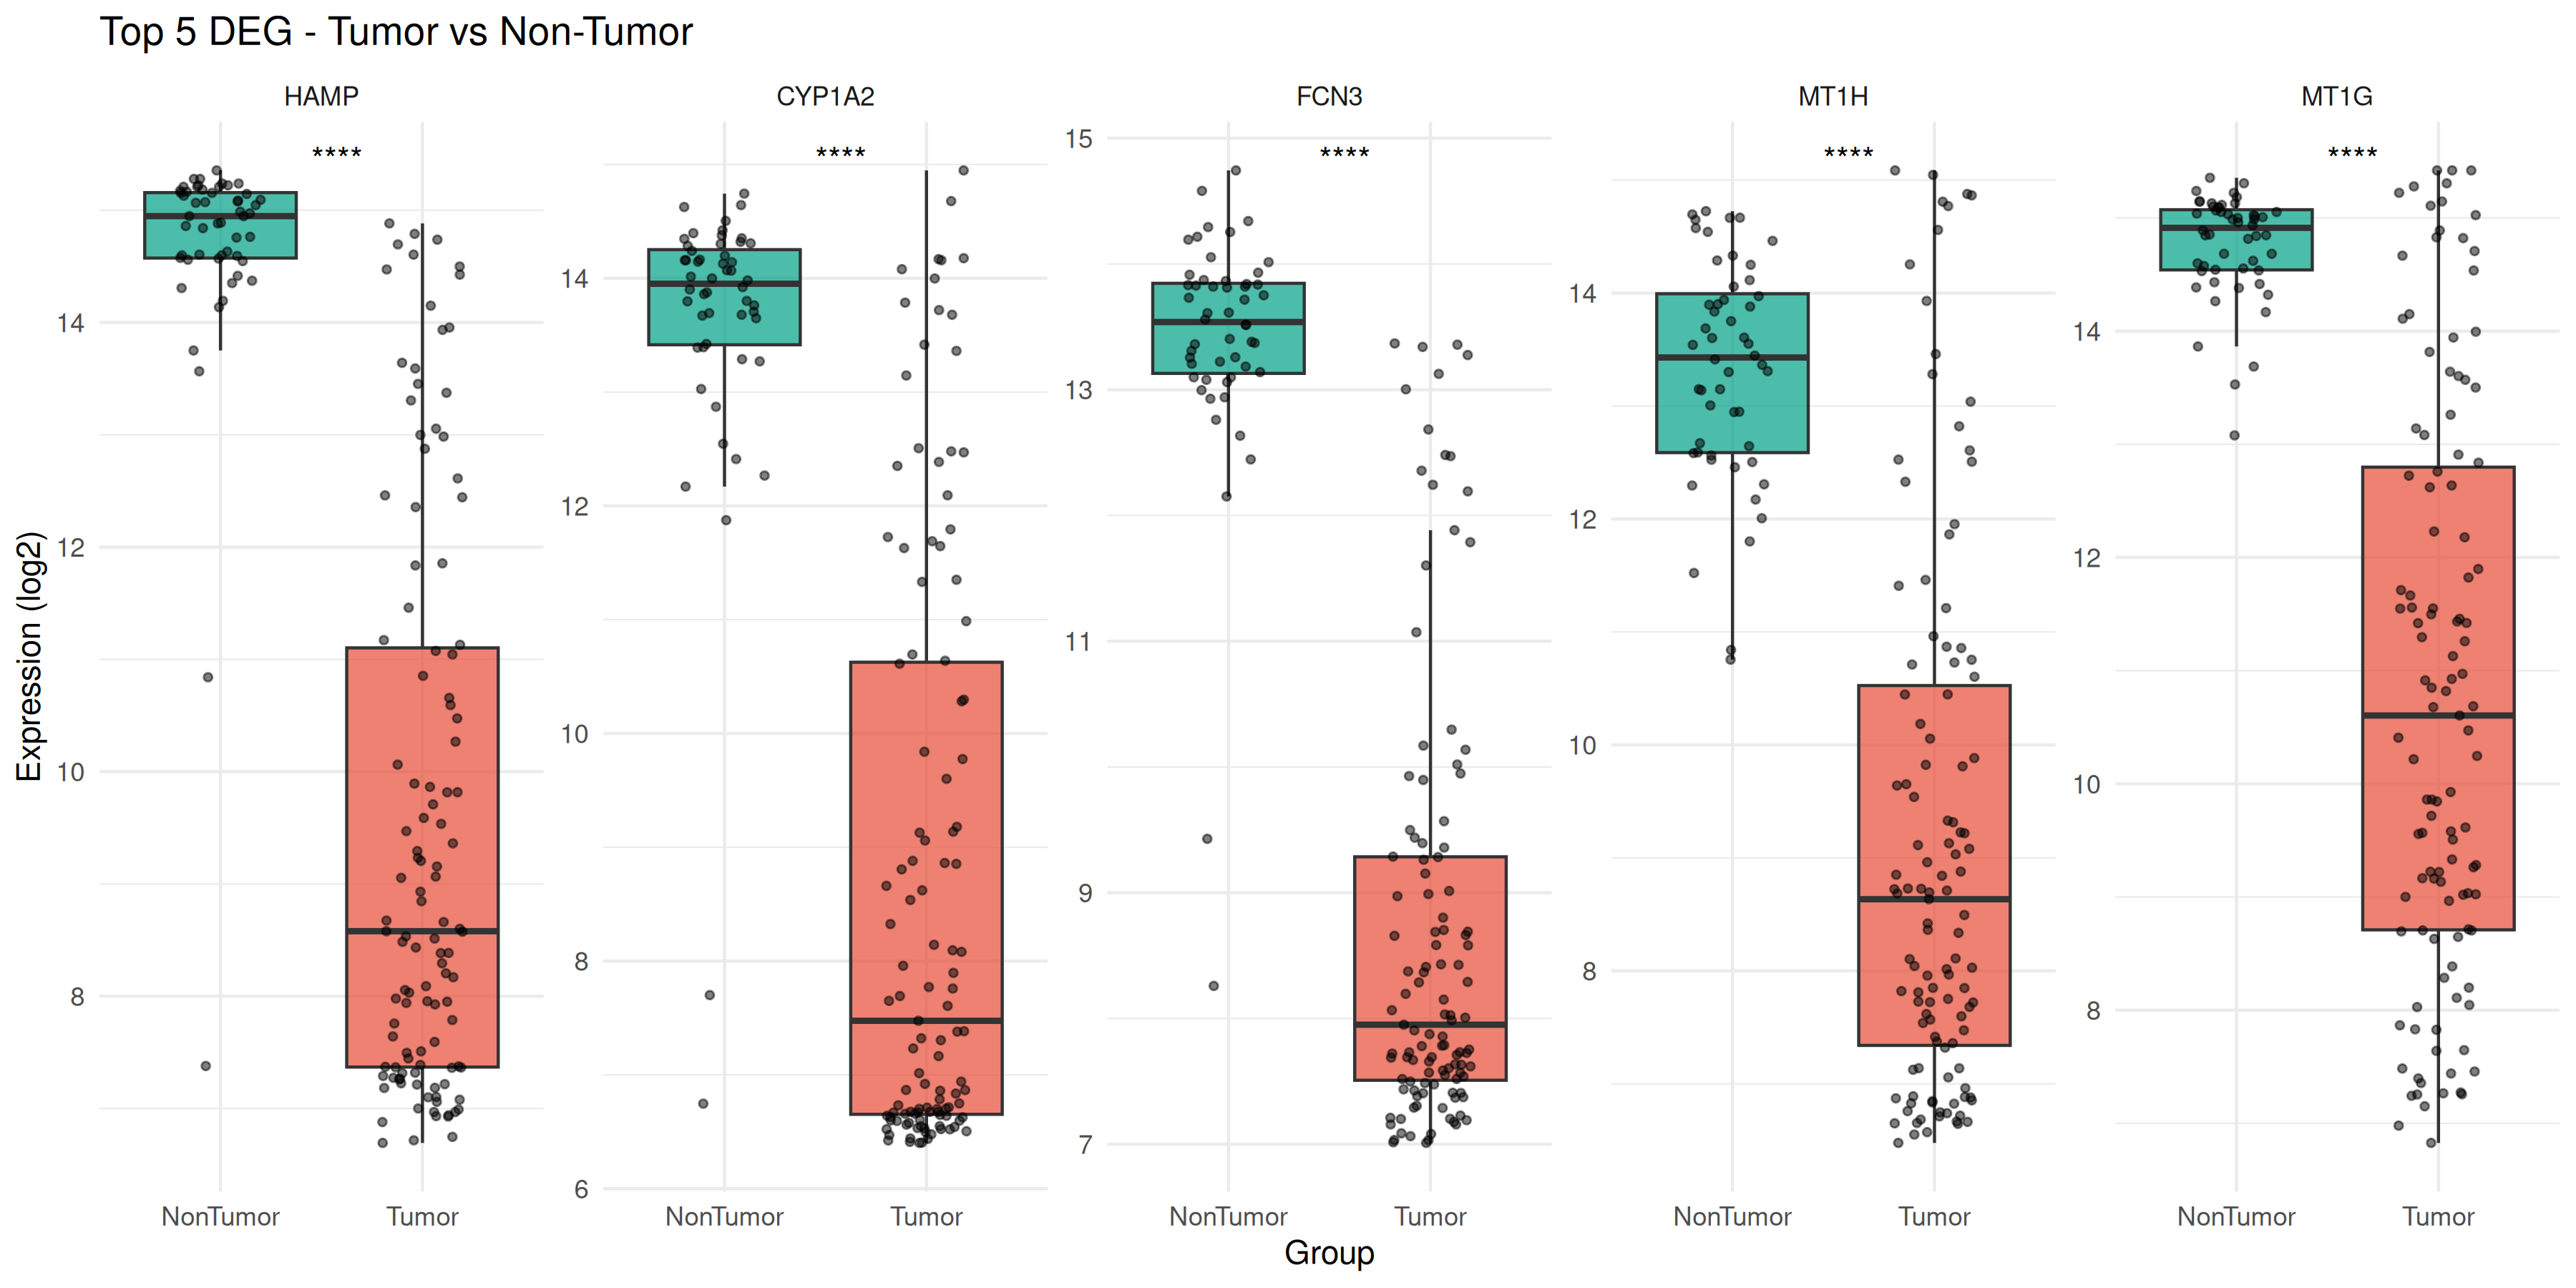
\includegraphics[width=0.95\textwidth]{boxplot_top5_with_stats.png}
\caption{En güçlü 5 DEG için kutu grafikleri}
\label{fig:boxtop5}
\end{figure}

\begin{figure}[H]
\centering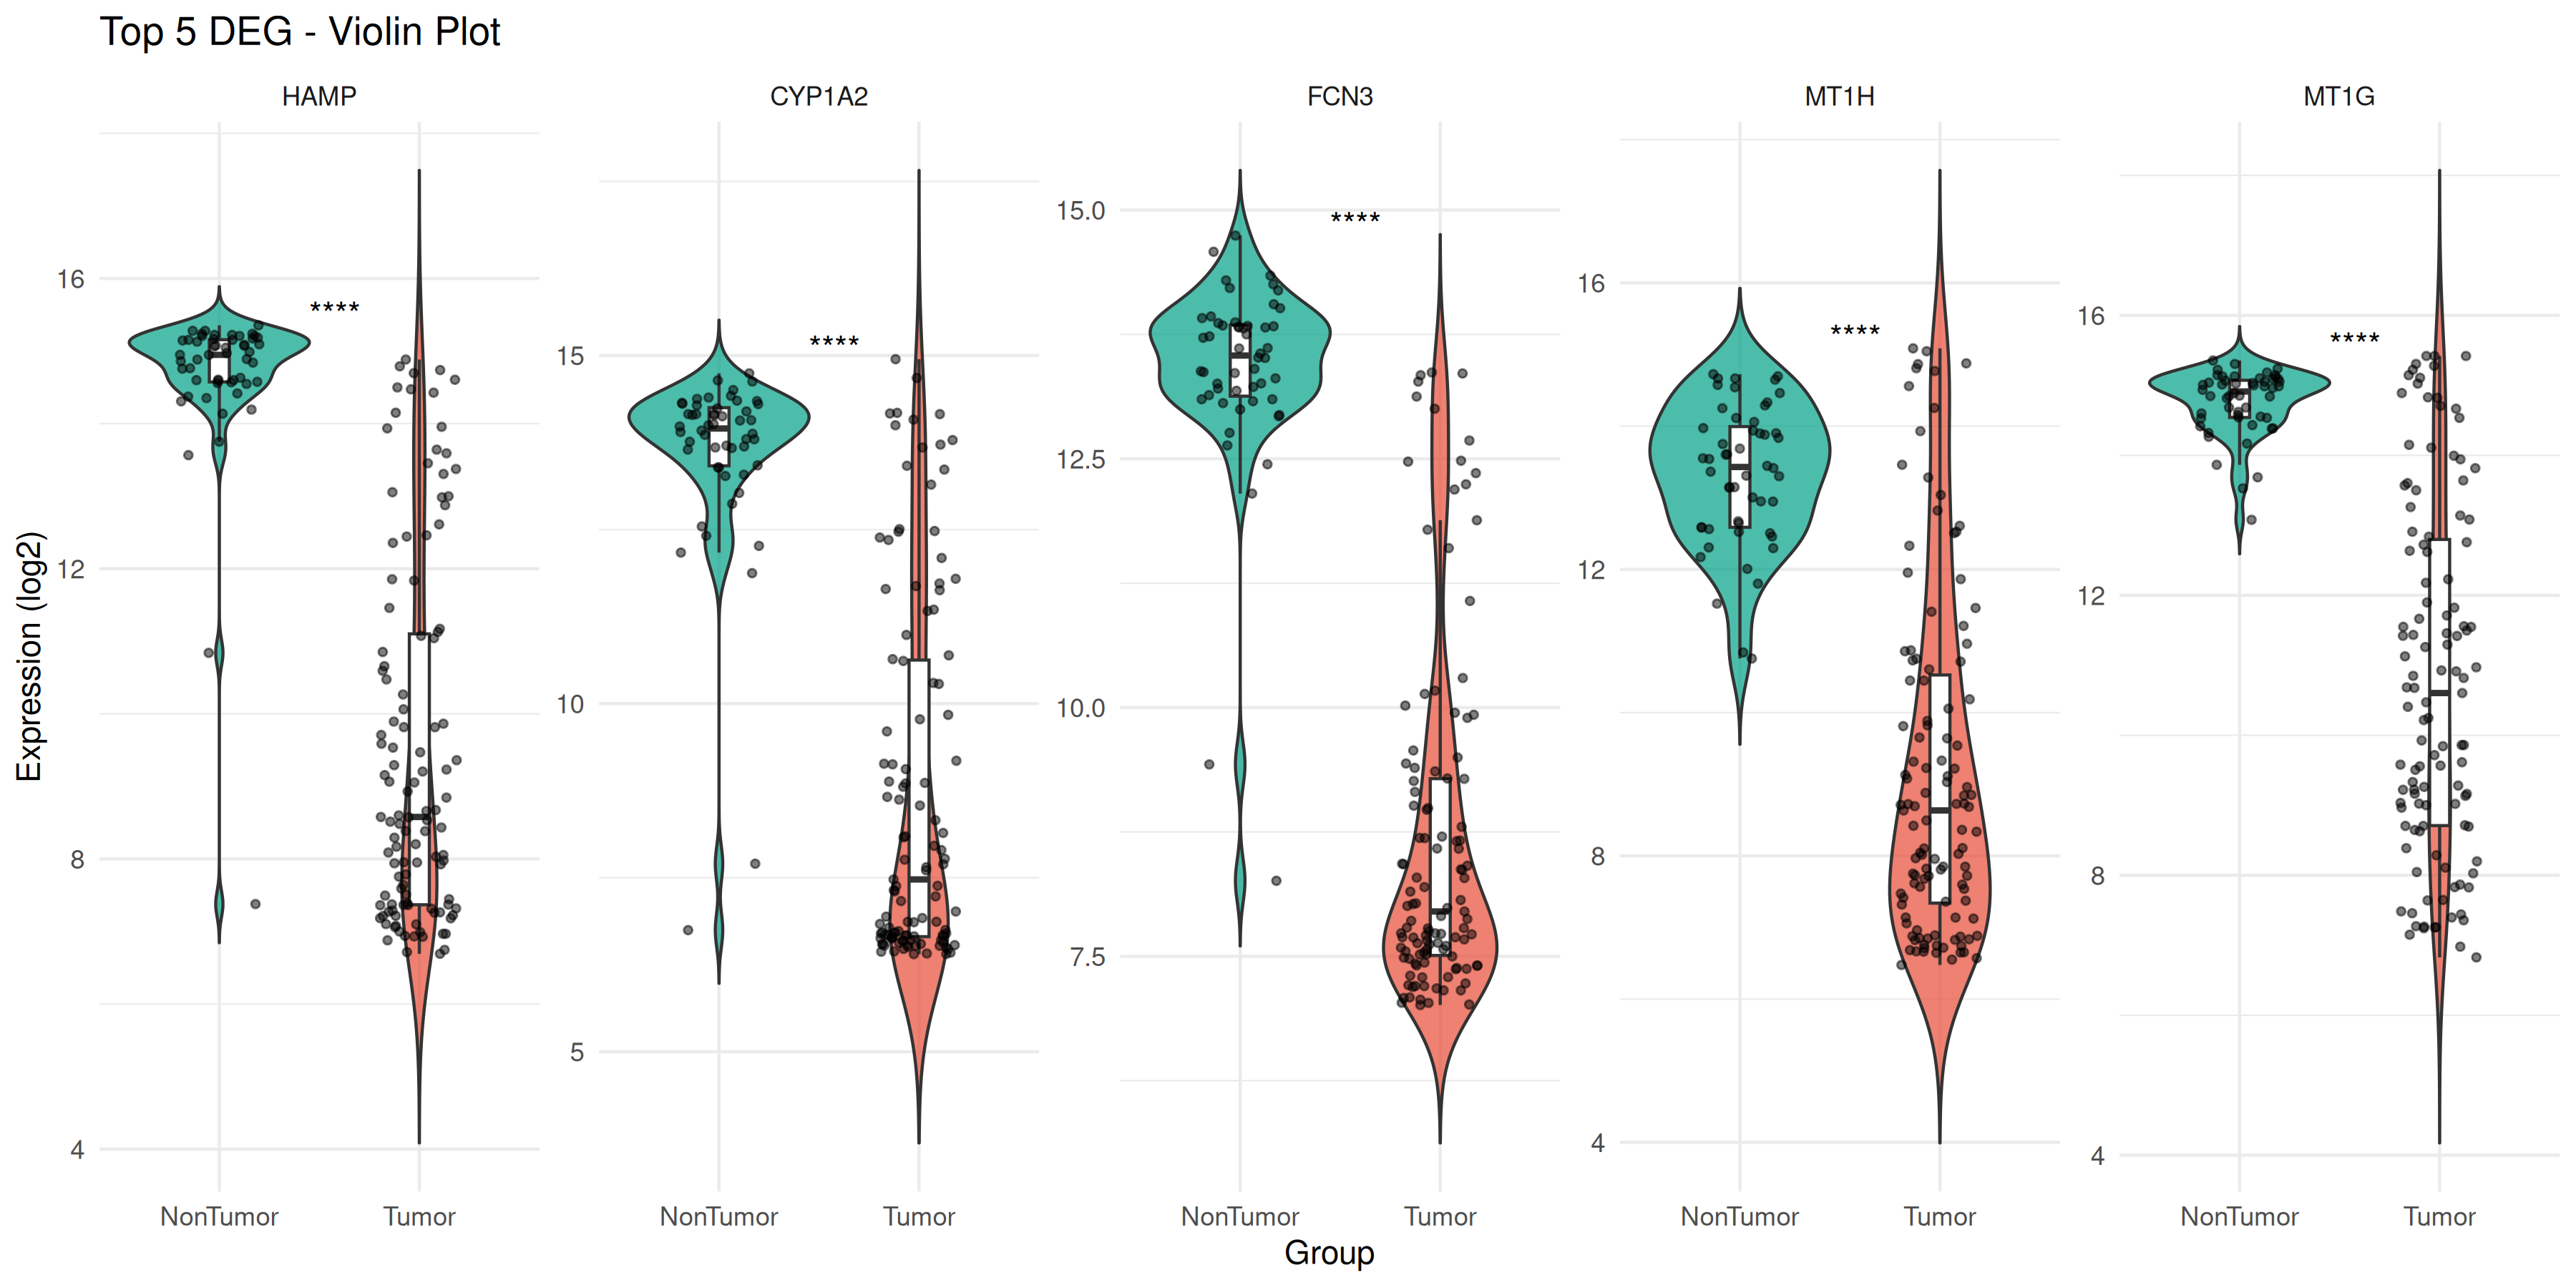
\includegraphics[width=0.95\textwidth]{violin_top5.png}
\caption{En güçlü 5 DEG için keman grafikleri}
\label{fig:violin}
\end{figure}

\begin{figure}[H]
\centering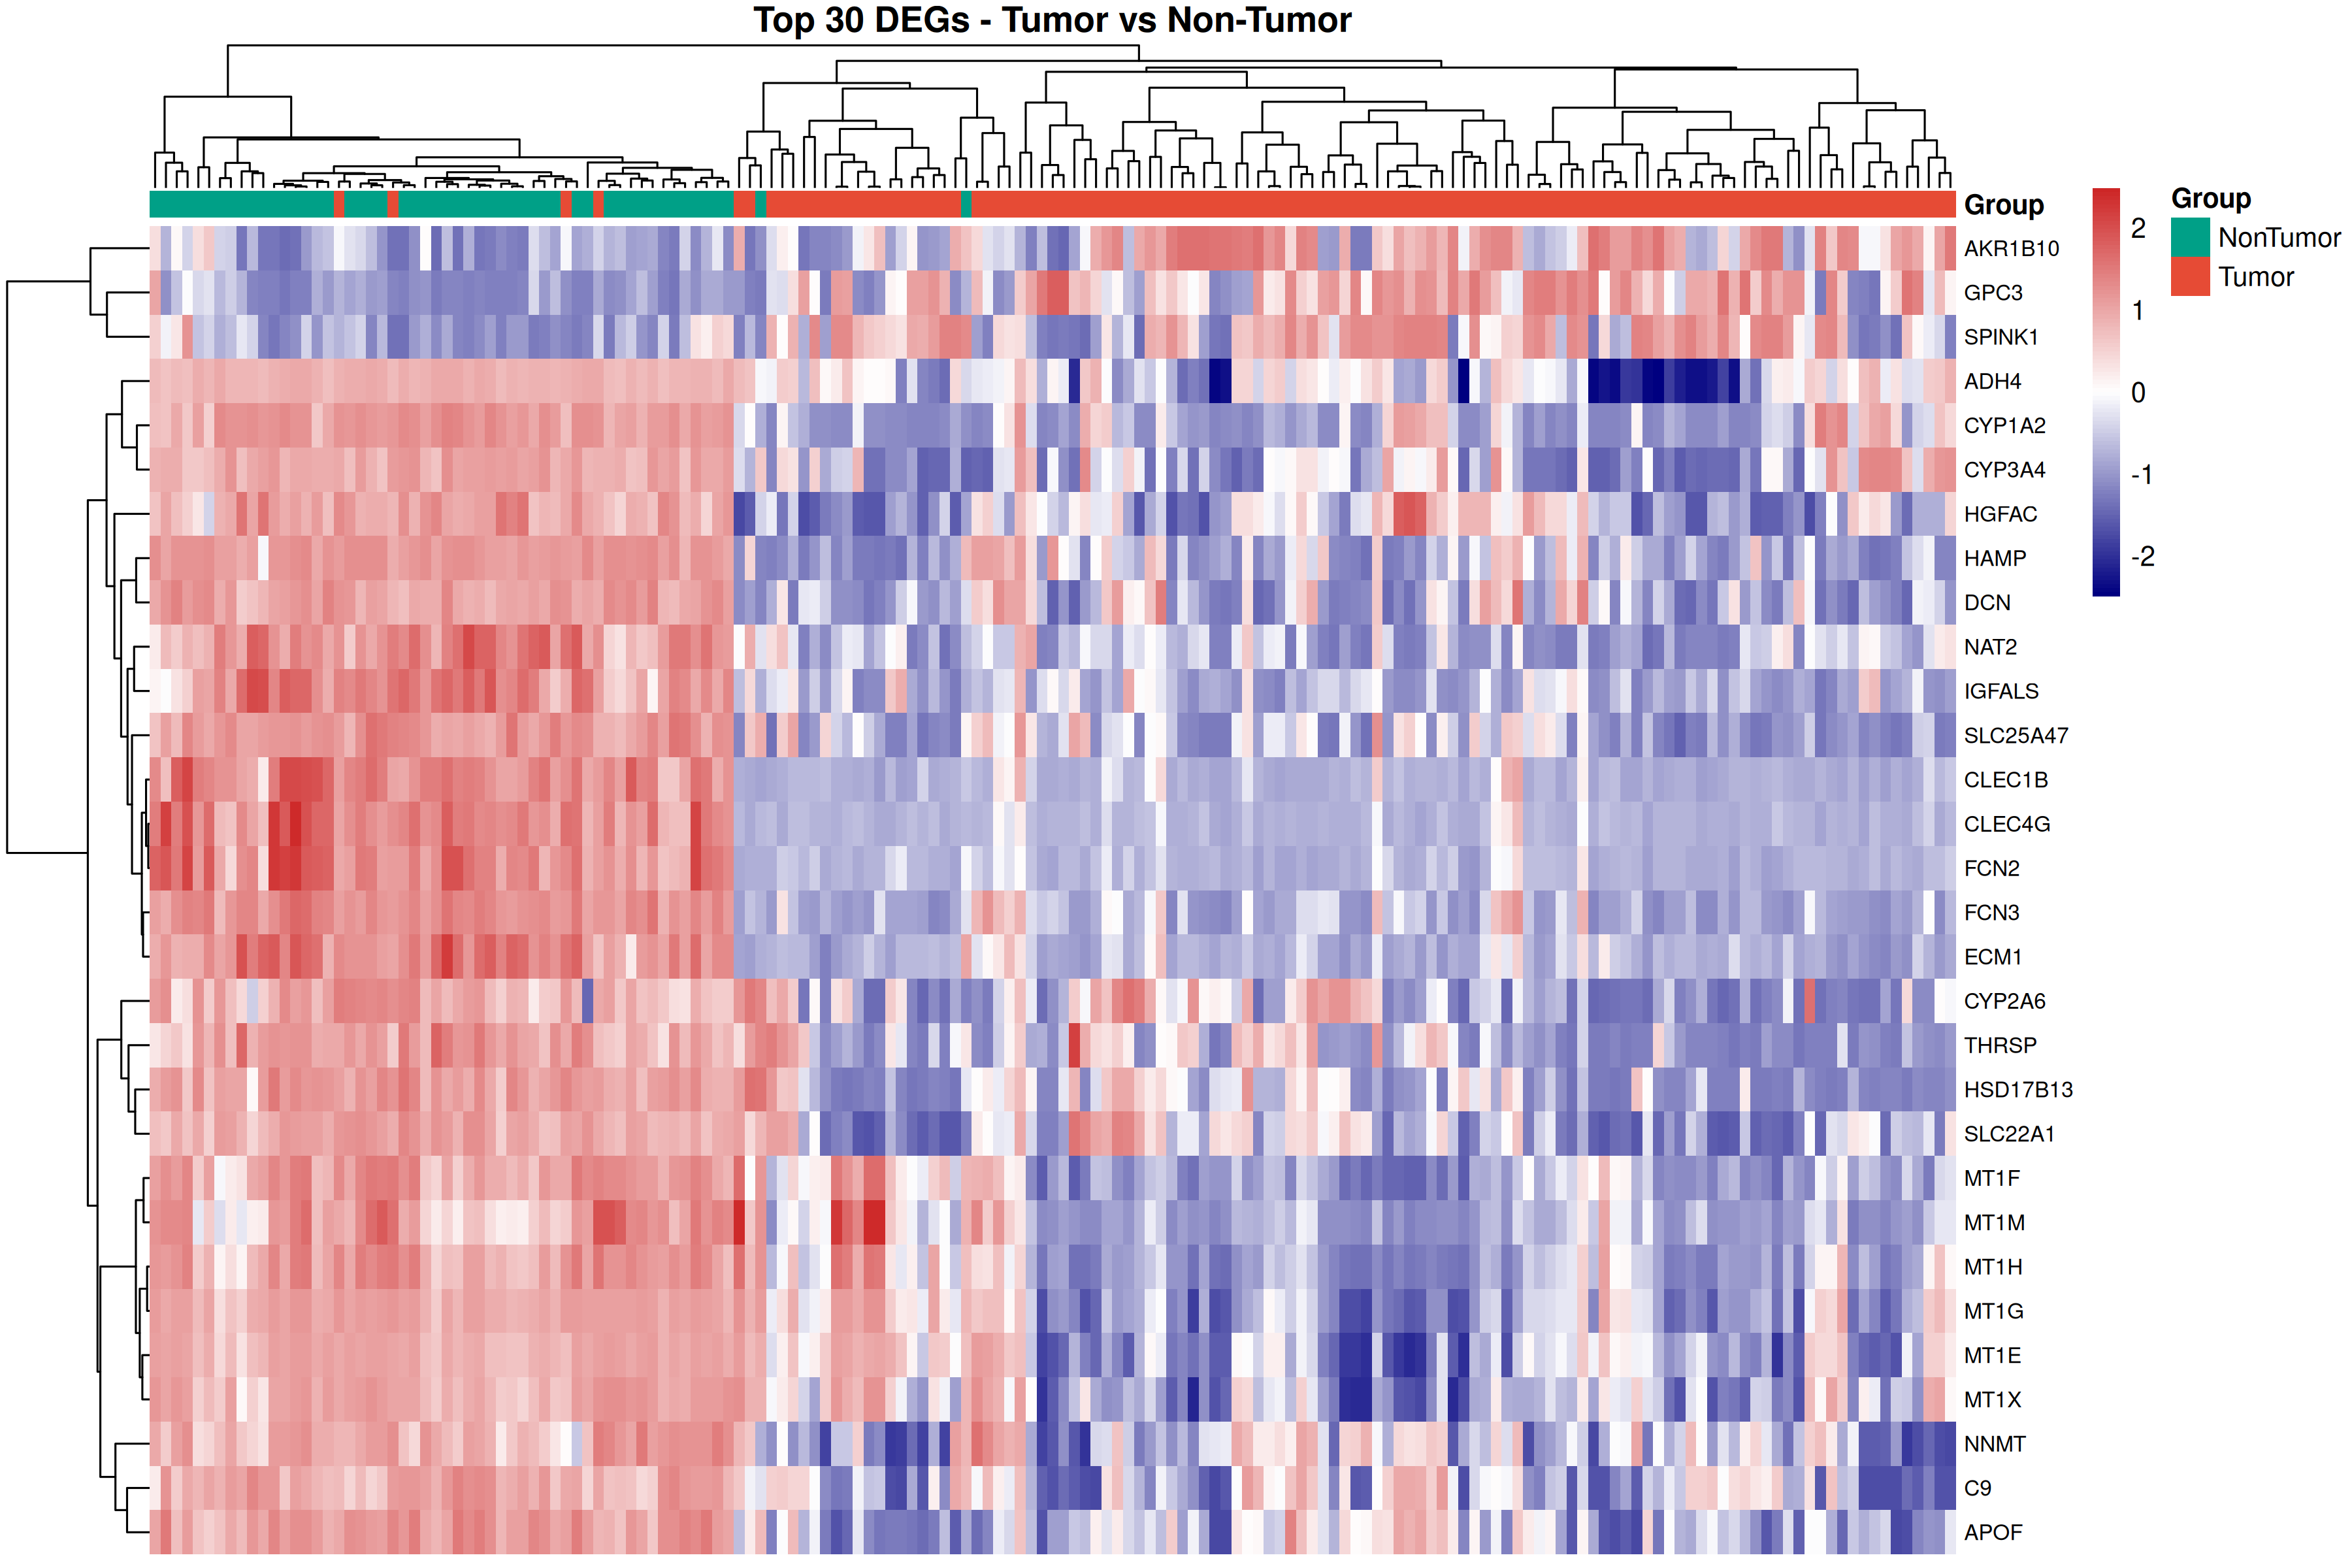
\includegraphics[width=0.85\textwidth]{heatmap_deg.png}
\caption{En anlamlı diferansiyel ifadeli genlerin ısı haritası}
\label{fig:heatmapdeg}
\end{figure}

\section{Biyolojik Yorum}

Down-regulated genler arasında HAMP, CYP1A2, FCN3, MT1H ve MT1G öne çıkmaktadır. Bu genler demir dengesi, ilaç metabolizması, bağışıklık yanıtı ve metal detoksifikasyonu gibi karaciğerin normal görevleriyle ilişkilidir. Bu nedenle tümör dokusunda bu genlerin daha düşük ifade göstermesi, normal karaciğer fonksiyonlarının azaldığını düşündürmektedir.

Up-regulated genler arasında ise GPC3, AKR1B10 ve TOP2A dikkat çekmektedir. Bu genler hücre çoğalması ve tümör gelişimiyle ilişkili süreçlerde rol oynayabilir. Özellikle GPC3'ün HCC tanısında bilinen bir gen belirteci olması, elde edilen DGE sonuçlarının biyolojik olarak tutarlı olduğunu göstermektedir.

% ------------------------------------------------------------------------------
\chapter{SURVIVAL ANALİZİ VE COX MODELİ}

\section{Yöntem}

Survival analizi yalnızca tümör örnekleri üzerinde yapılmıştır. Ana değerlendirme ölçütü genel sağkalım (OS) olarak seçilmiştir. Bu analizde 115 tümör örneği kullanılmış ve 23 ölüm olayı bulunmaktadır. 

DGE analizinden seçilen en güçlü 5 up-regulated ve 5 down-regulated gen olmak üzere toplam 10 gen incelenmiştir. Her gen için örnekler, gen ifade değerinin medyanına göre yüksek ifade ve düşük ifade gruplarına ayrılmıştır. Bu gruplar Kaplan-Meier eğrileri ve log-rank testi ile karşılaştırılmıştır.

Ek olarak, gen ifade grubu, yaş ve cinsiyet değişkenleri kullanılarak Cox regresyon modeli kurulmuştur. Tekrarsız sağkalım (RFS) ikincil olarak değerlendirilmiş, ancak düzeltilmiş örnek eşleştirmesi sonrasında RFS için anlamlı bir gen bulunmamıştır.

\section{Sonuçlar}

Kaplan-Meier log-rank test sonuçları Tablo~\ref{tab:survival} içinde verilmiştir. Üç gen anlamlı bulunmuştur: \textbf{MT1G} (p = 0,006), \textbf{MT1H} (p = 0,023) ve \textbf{AKR1B10} (p = 0,039).

\begin{table}[H]
\centering
\caption{Kaplan-Meier sağkalım analizi sonuçları (OS)}
\label{tab:survival}
\begin{tabular}{llr}
\toprule
\textbf{Gen} & \textbf{Yön} & \textbf{p-değeri} \\
\midrule
\textbf{MT1G} & Down & \textbf{0,006} \\
\textbf{MT1H} & Down & \textbf{0,023} \\
\textbf{AKR1B10} & Up & \textbf{0,039} \\
FCN3 & Down & 0,087 \\
GPC3 & Up & 0,633 \\
SPINK1 & Up & 0,403 \\
TOP2A & Up & 0,468 \\
ACSL4 & Up & 0,474 \\
CYP1A2 & Down & 0,460 \\
HAMP & Down & 0,680 \\
\bottomrule
\end{tabular}
\end{table}

En anlamlı gen olan MT1G'ye ait Kaplan-Meier eğrisi Şekil~\ref{fig:kmmt1g}, Cox modeli forest plot grafiği Şekil~\ref{fig:forestmt1g} ile verilmiştir.

\begin{figure}[H]
\centering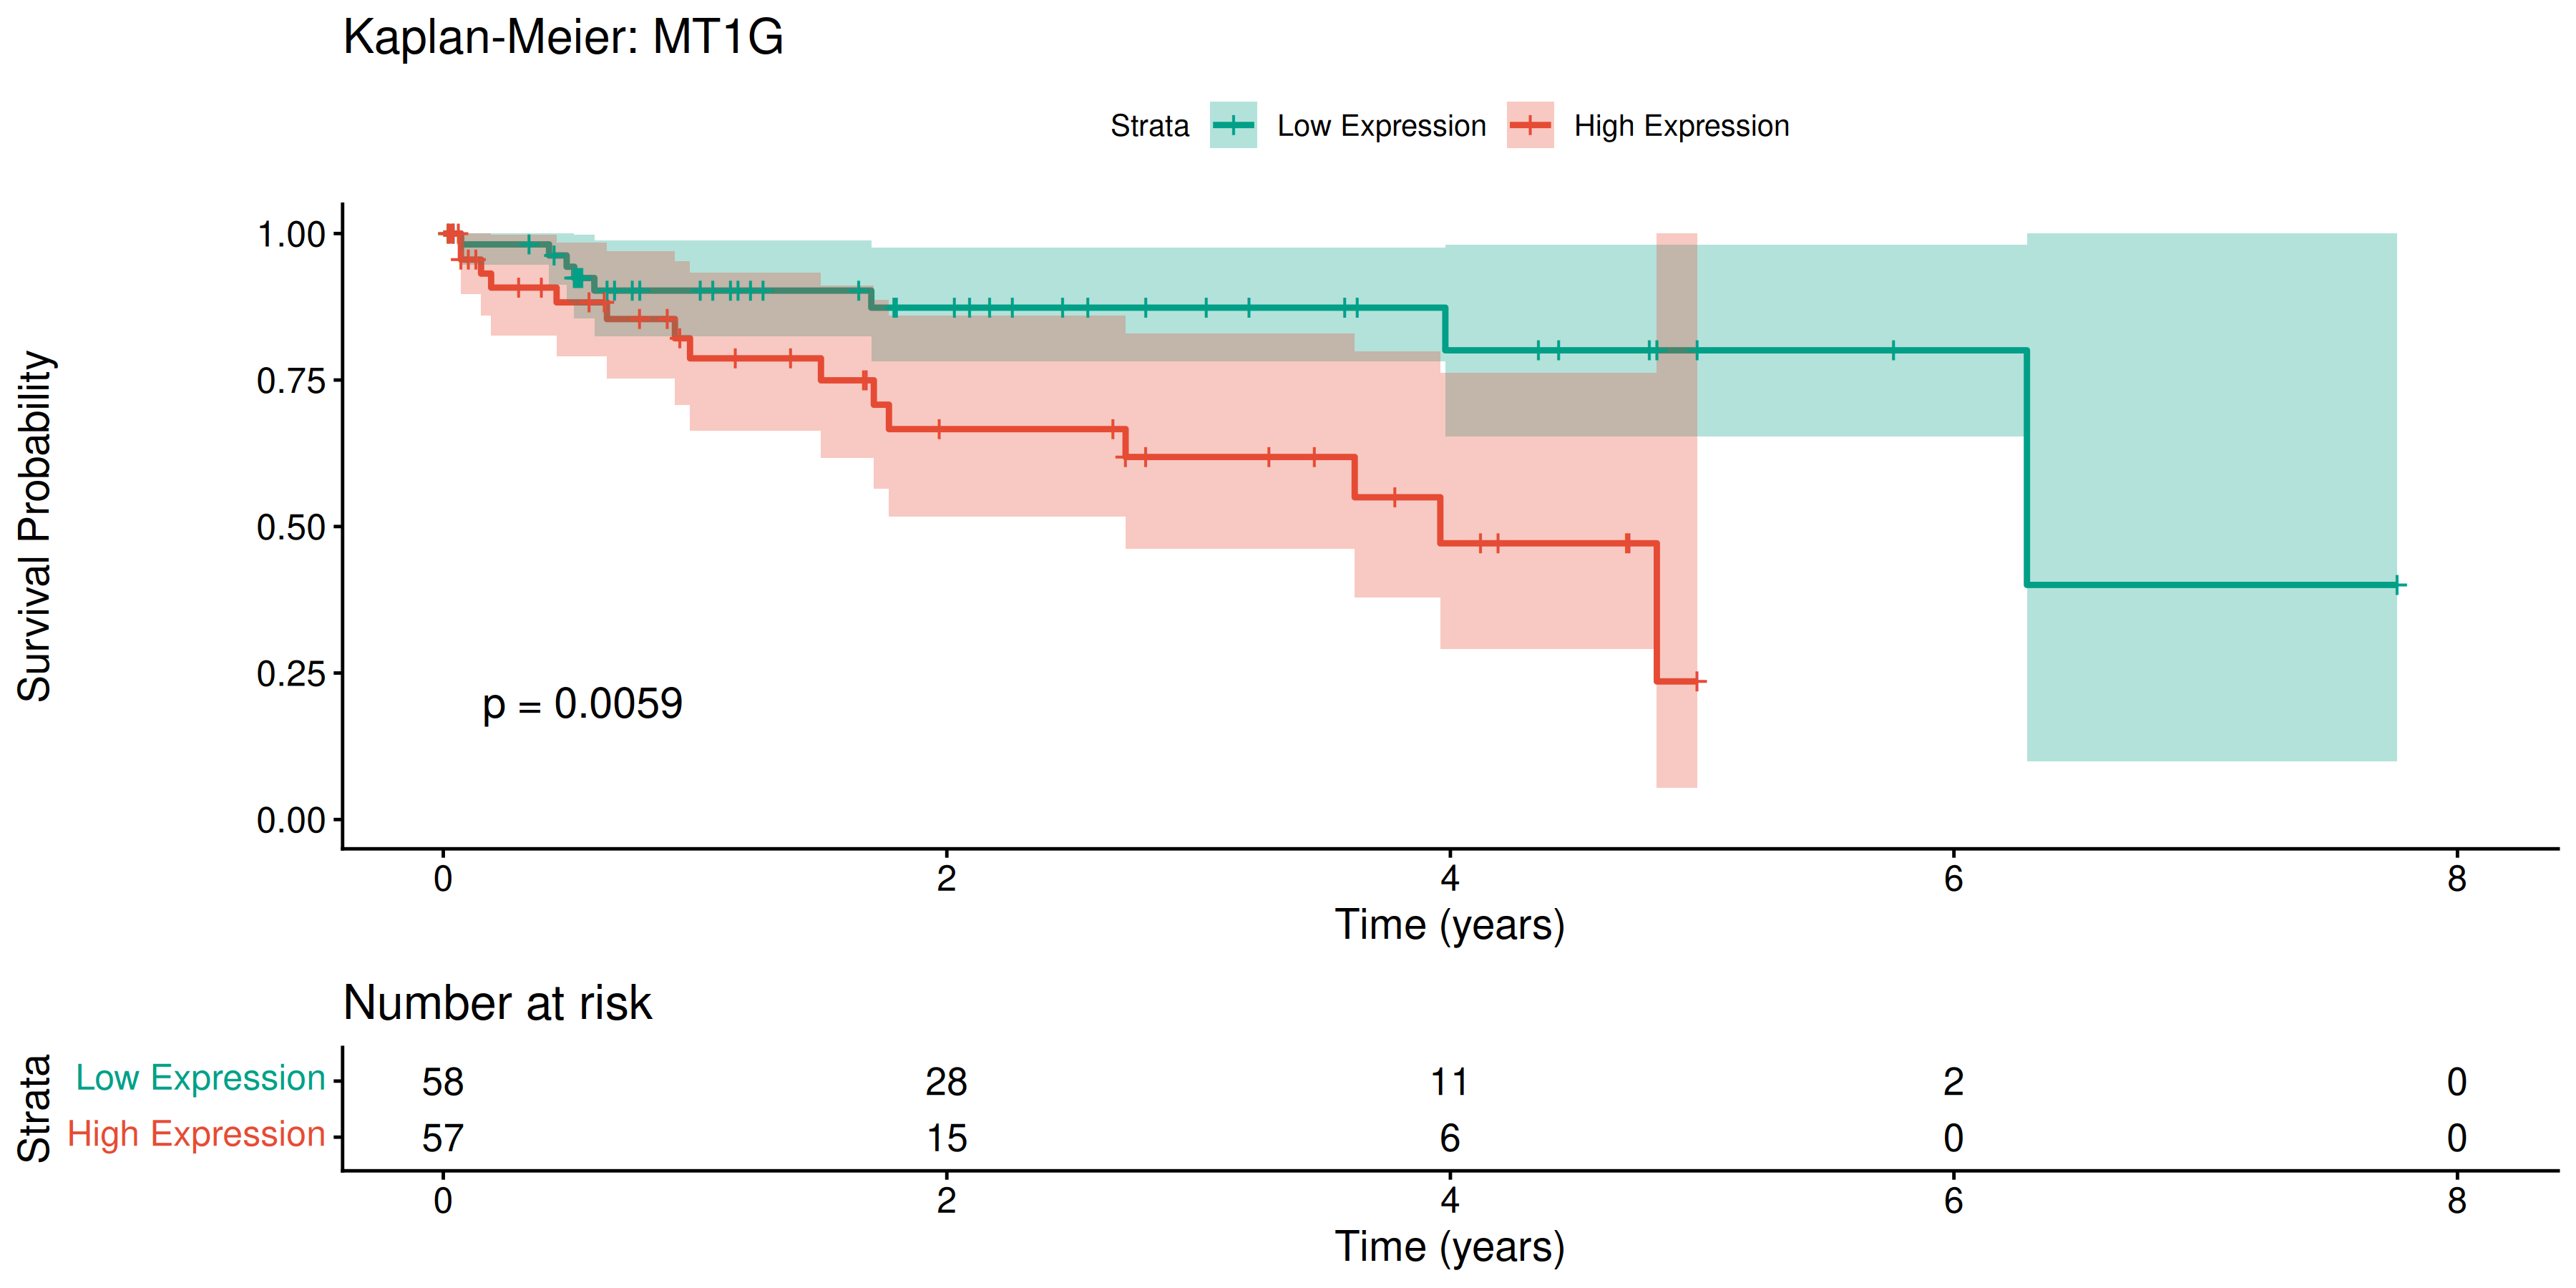
\includegraphics[width=0.9\textwidth]{km_MT1G.png}
\caption{MT1G geni için Kaplan-Meier genel sağkalım (OS) eğrisi}
\label{fig:kmmt1g}
\end{figure}

\begin{figure}[H]
\centering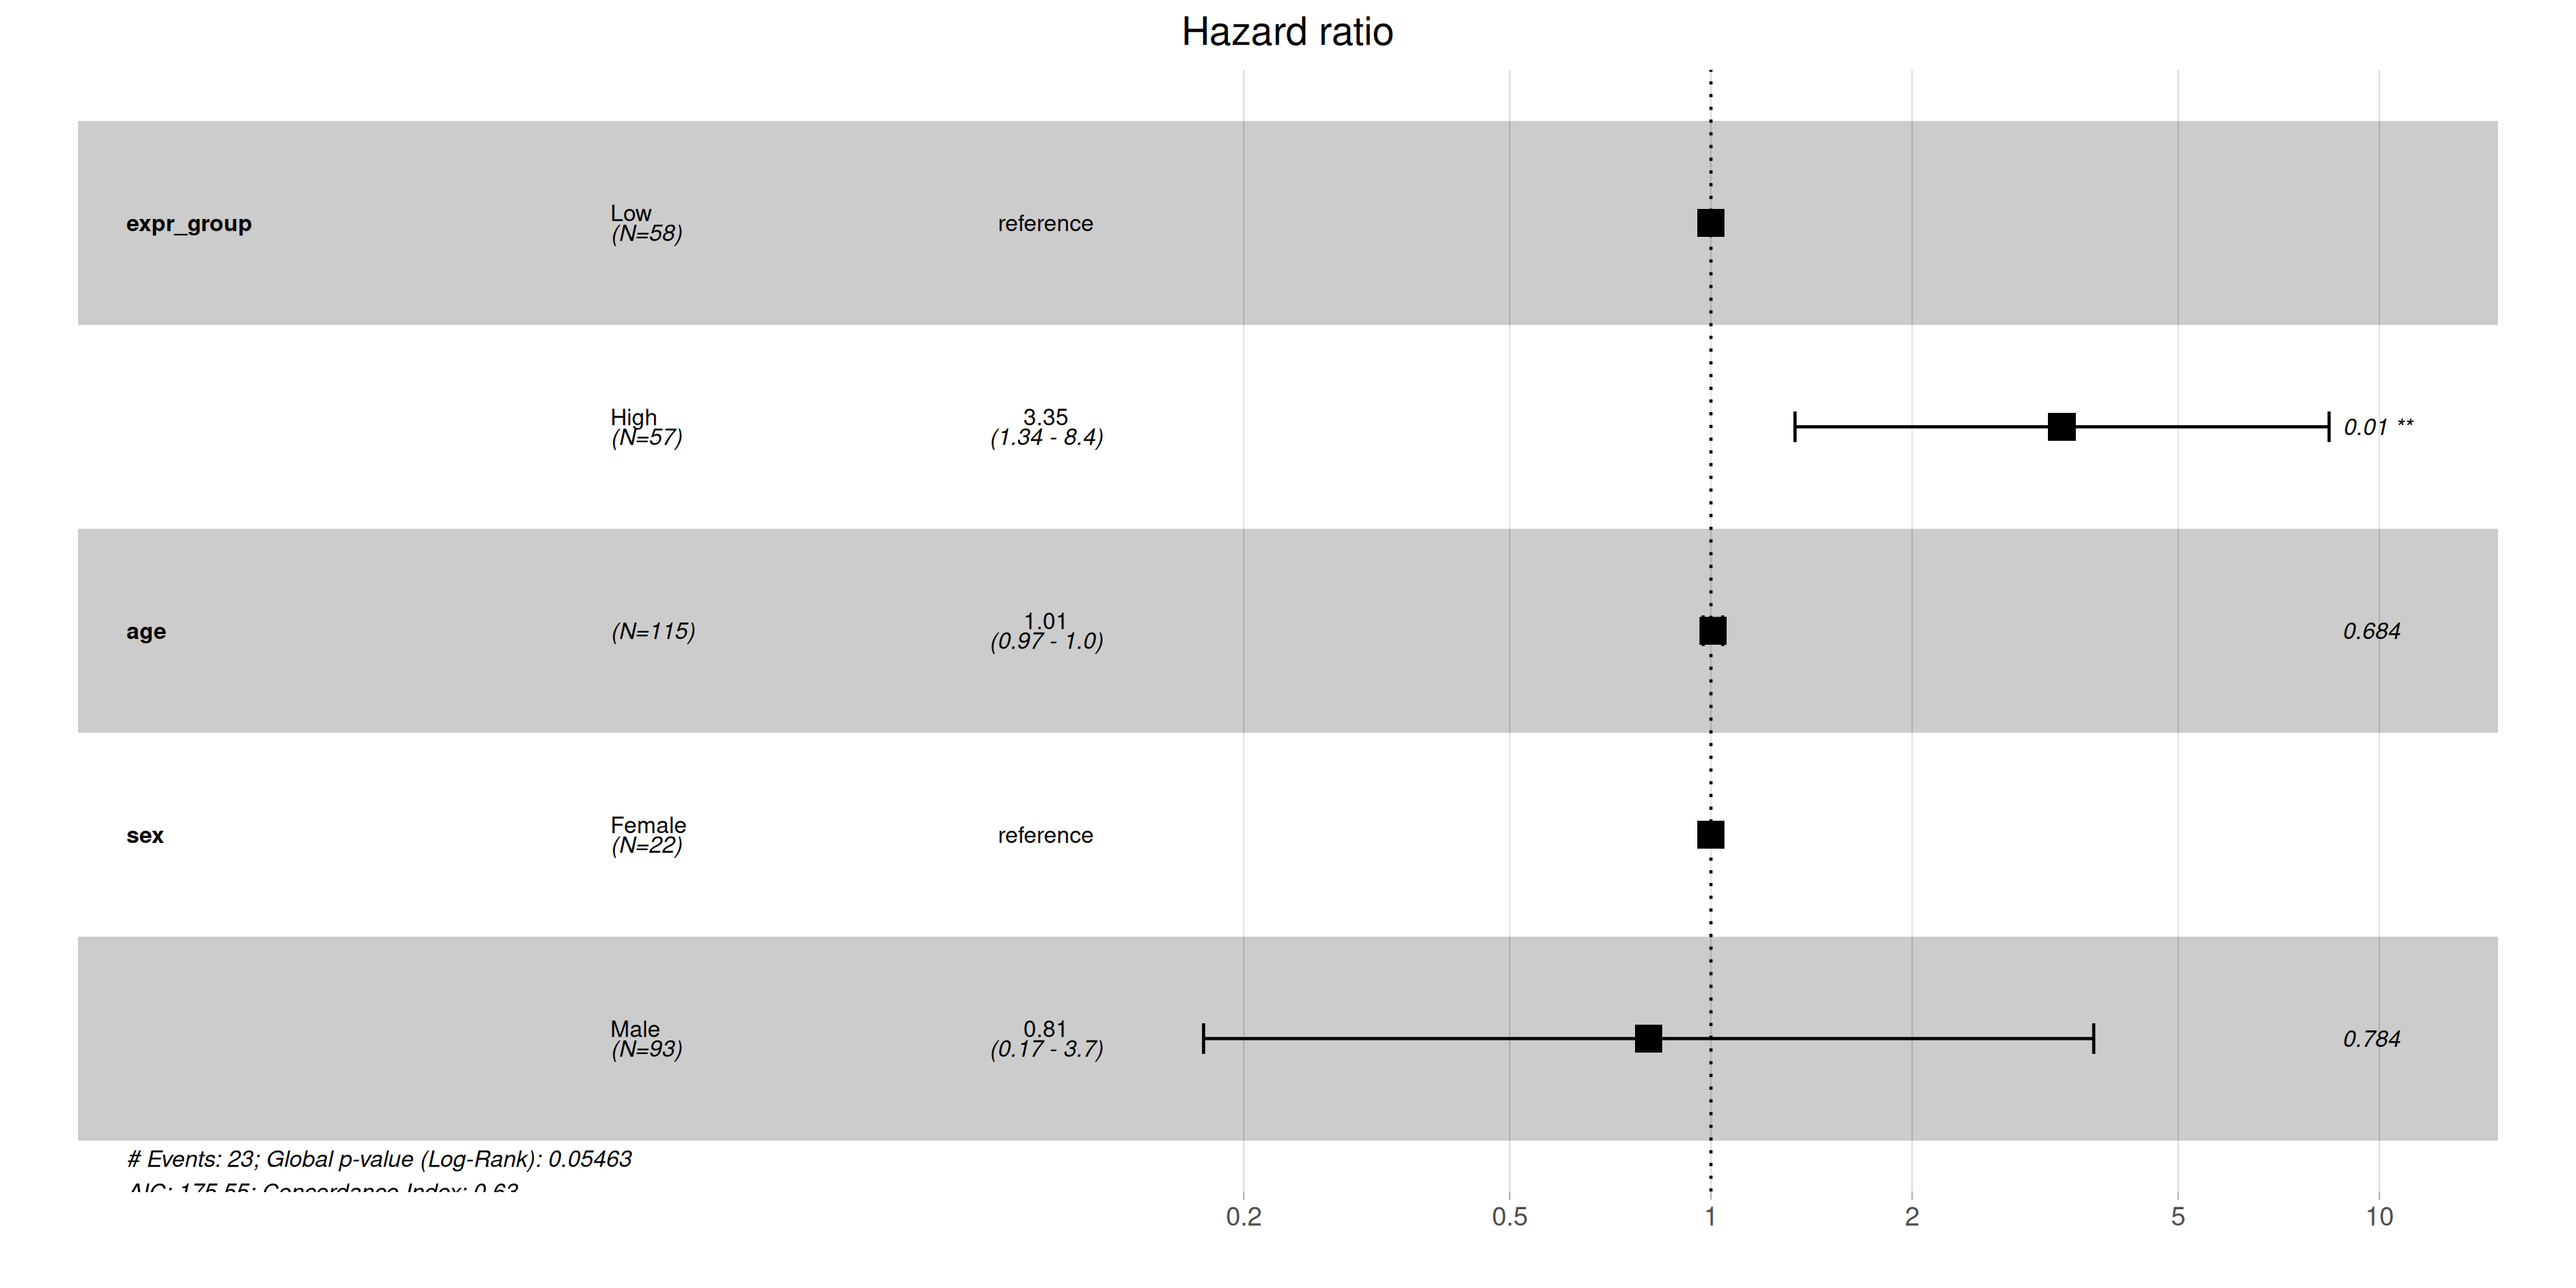
\includegraphics[width=0.9\textwidth]{forest_MT1G.png}
\caption{MT1G geni için Cox regresyon forest plot grafiği}
\label{fig:forestmt1g}
\end{figure}

\section{Yorum}

Cox modelinde yüksek MT1G ifade grubunun ölüm riski daha yüksek bulunmuştur (HR = 3,35; \%95 GA 1,34--8,41; p = 0,010). Benzer şekilde MT1H için de daha yüksek risk gözlenmiştir (HR = 2,65; p = 0,029). AKR1B10 ise koruyucu yönde bir eğilim göstermiştir, ancak bu sonuç sınırda anlamlıdır (HR = 0,41; p = 0,052).

MT1G ve MT1H tümör dokusunda genel olarak daha düşük ifade edilen genlerdir. Buna rağmen, tümör örnekleri içinde bu genlerin daha yüksek ifade edilmesi sağkalım ile ilişkili bulunmuştur. Cox modeline yaş ve cinsiyet dahil edilmiş; olay sayısı düşük olduğu için BCLC evresi modele eklenmemiştir. Metadata'da sigara ve alkol bilgisi bulunmadığından bu değişkenler değerlendirilememiştir.

% ------------------------------------------------------------------------------
\chapter{WGCNA ANALİZİ}

\section{Yöntem}

WGCNA, benzer ifade örüntüsüne sahip genleri aynı gruplar altında toplayan bir ağ analizi yöntemidir. Bu analizde Top-3000 yüksek varyanslı gen kullanılmıştır.

Ağ yapısını oluşturmak için önce genler arasındaki ilişki düzeyi hesaplanmıştır. Daha sonra ölçeksiz topolojiye uygunluğu sağlayan Soft Thresholding gücü $\beta = 5$ olarak seçilmiştir (Şekil~\ref{fig:soft}). Bu değer kullanılarak genler arasındaki bağlantılar hesaplanmış ve benzer bağlantı yapısına sahip genler modüller halinde gruplandırılmıştır.

\begin{figure}[H]
\centering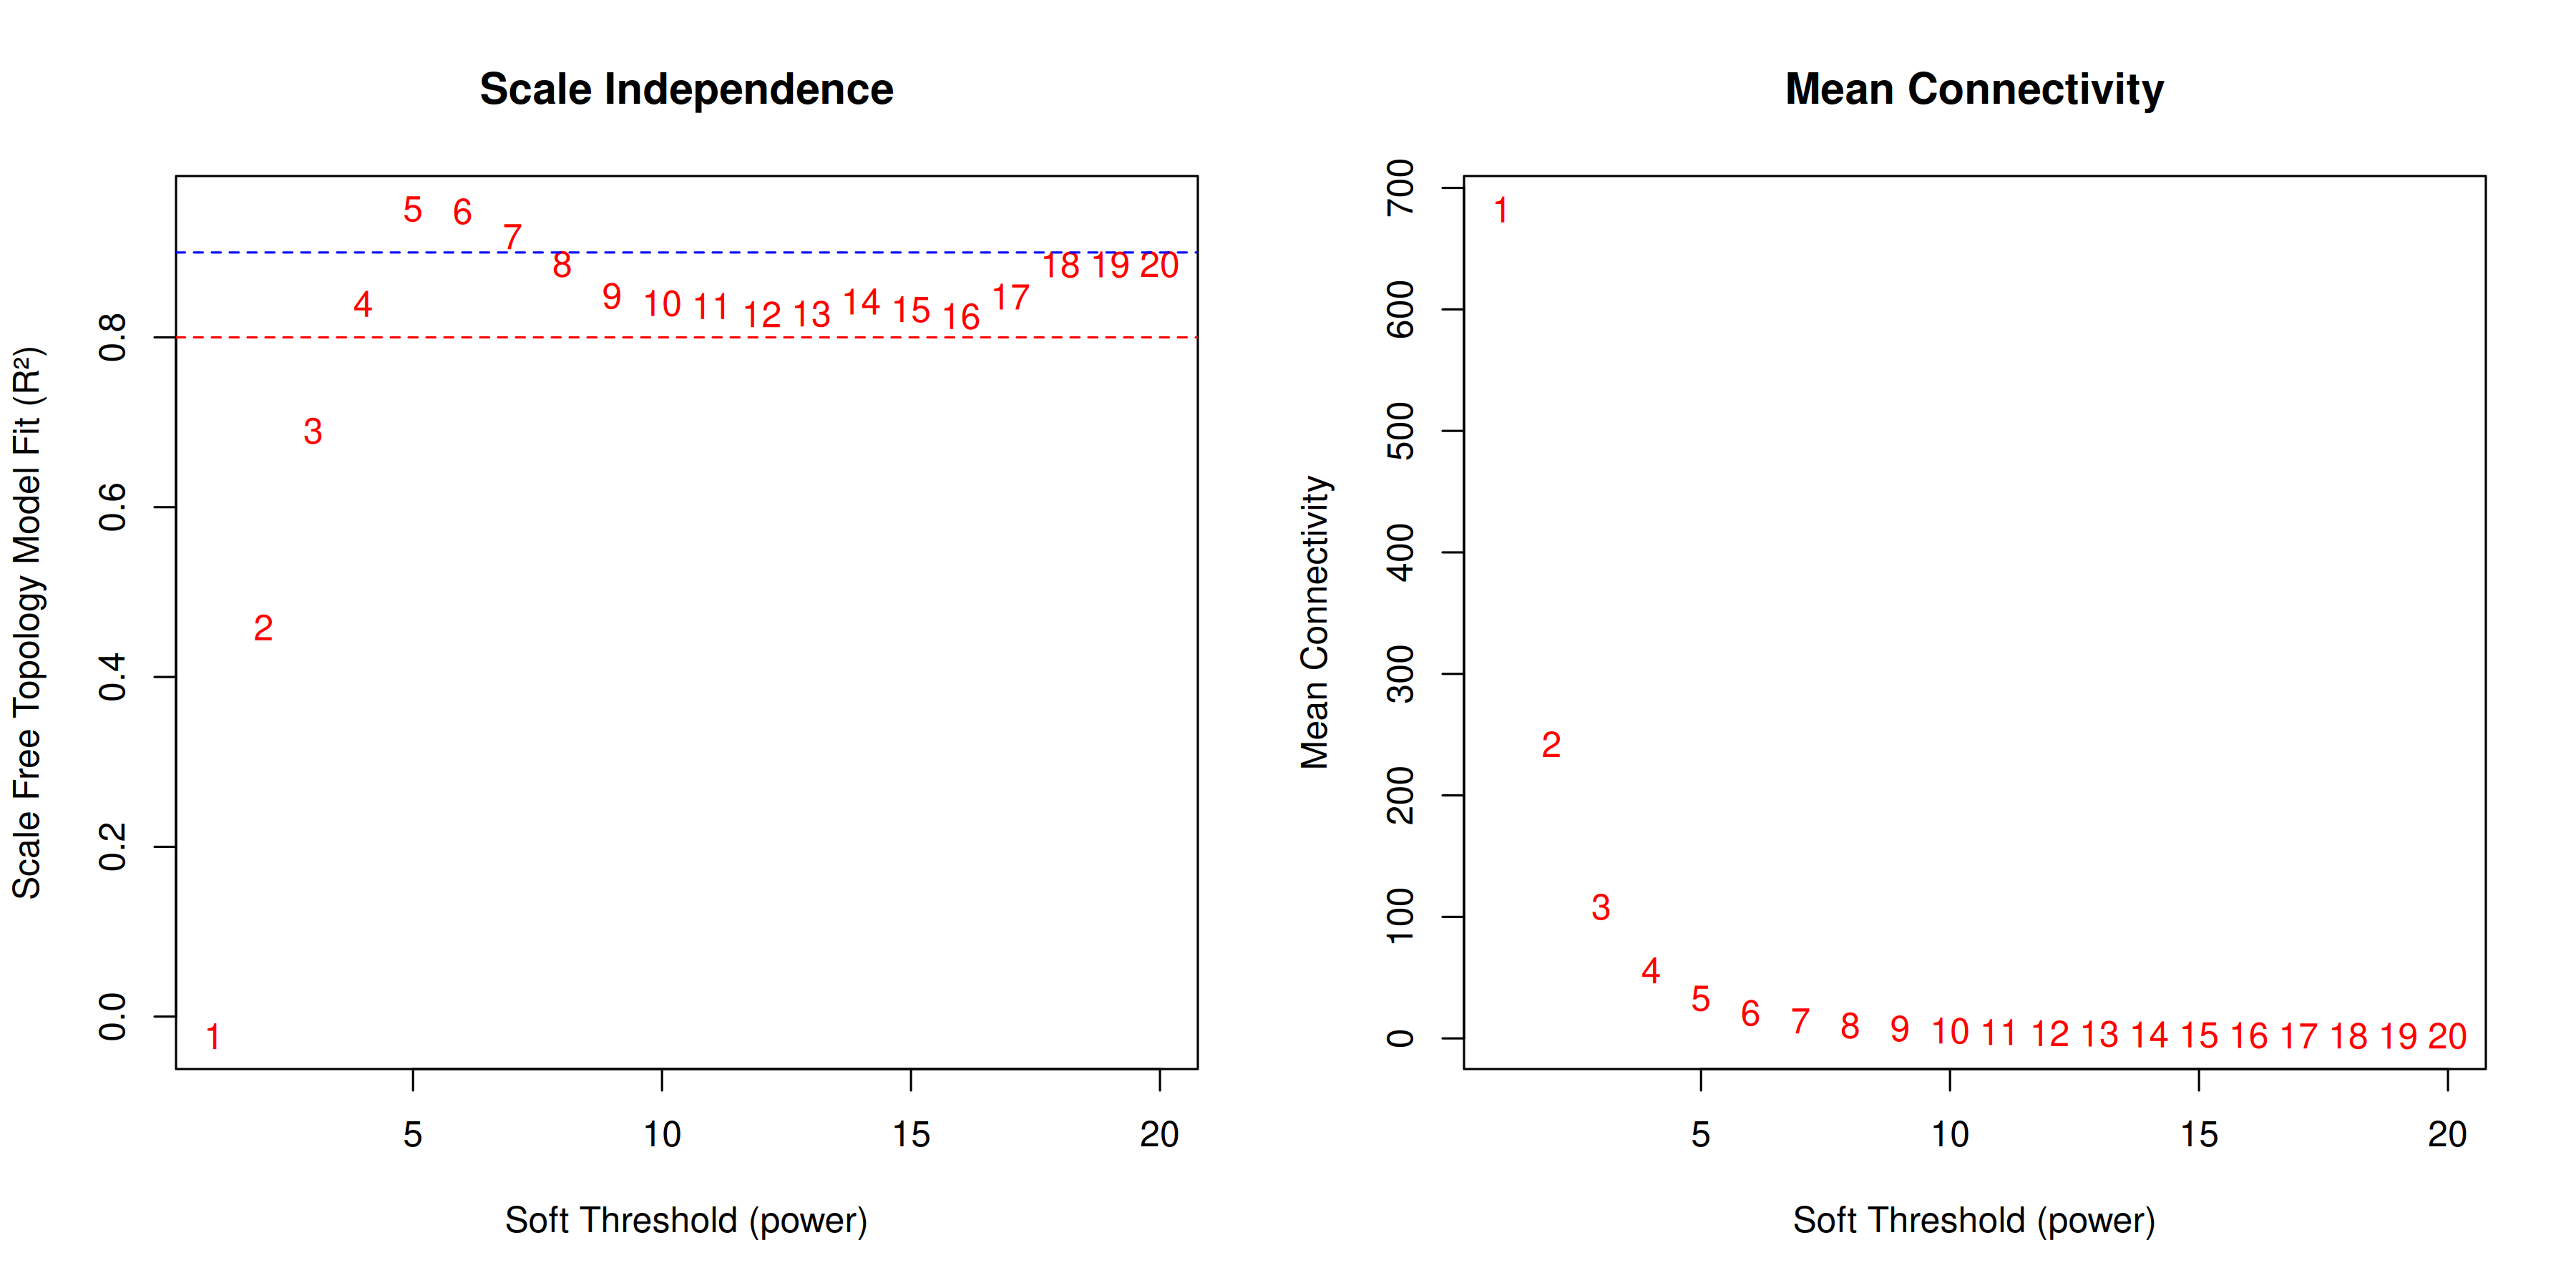
\includegraphics[width=0.95\textwidth]{soft_threshold.png}
\caption{Soft Threshold güç seçimi: ölçeksiz topoloji uyumu ve ortalama bağlantısallık}
\label{fig:soft}
\end{figure}

\section{Modül Tespiti ve Modül-Trait İlişkisi}

Analiz sonucunda 6 gen modülü belirlenmiştir (Şekil~\ref{fig:dendro}). Daha sonra bu modüllerin tümör/non-tümör durumu ve klinik değişkenlerle ilişkisi incelenmiştir (Şekil~\ref{fig:modtrait}).

Bu karşılaştırmada \textbf{brown modülü} 1636 gen içermekte ve tümör/non-tümör ayrımıyla en güçlü ilişkiyi göstermektedir. Bu nedenle sonraki hub gen ve GO analizlerinde brown modülü seçilmiştir.

\begin{figure}[H]
\centering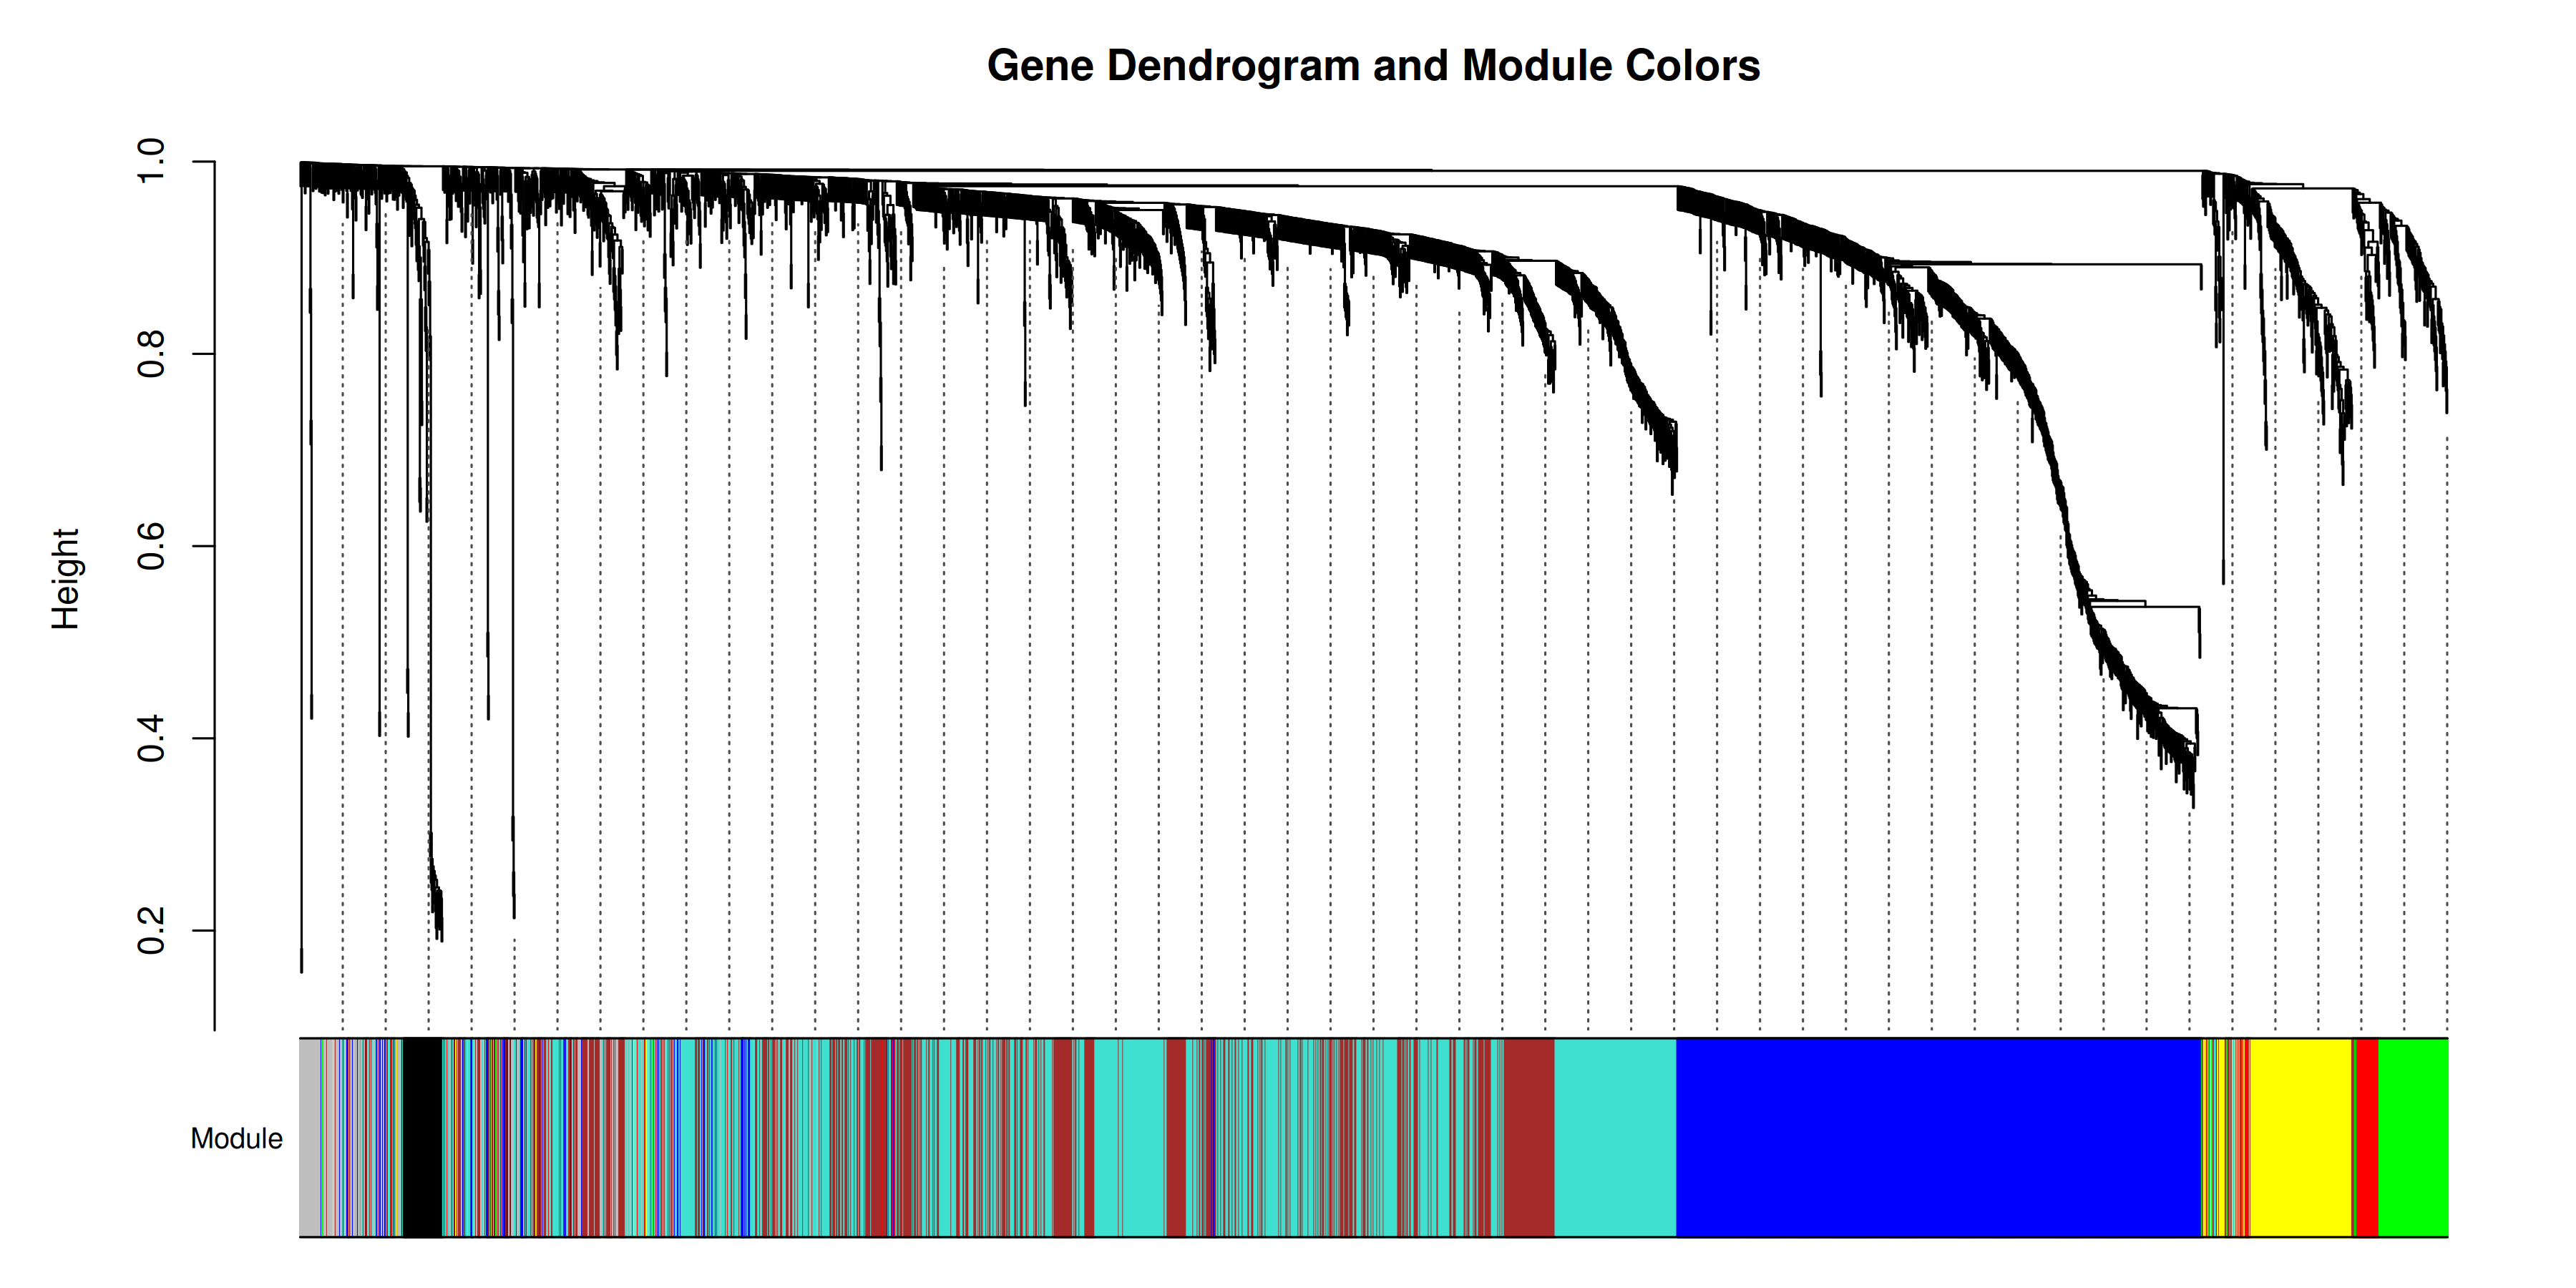
\includegraphics[width=0.95\textwidth]{gene_dendrogram.png}
\caption{Gen dendrogramı ve modül renkleri}
\label{fig:dendro}
\end{figure}

\begin{figure}[H]
\centering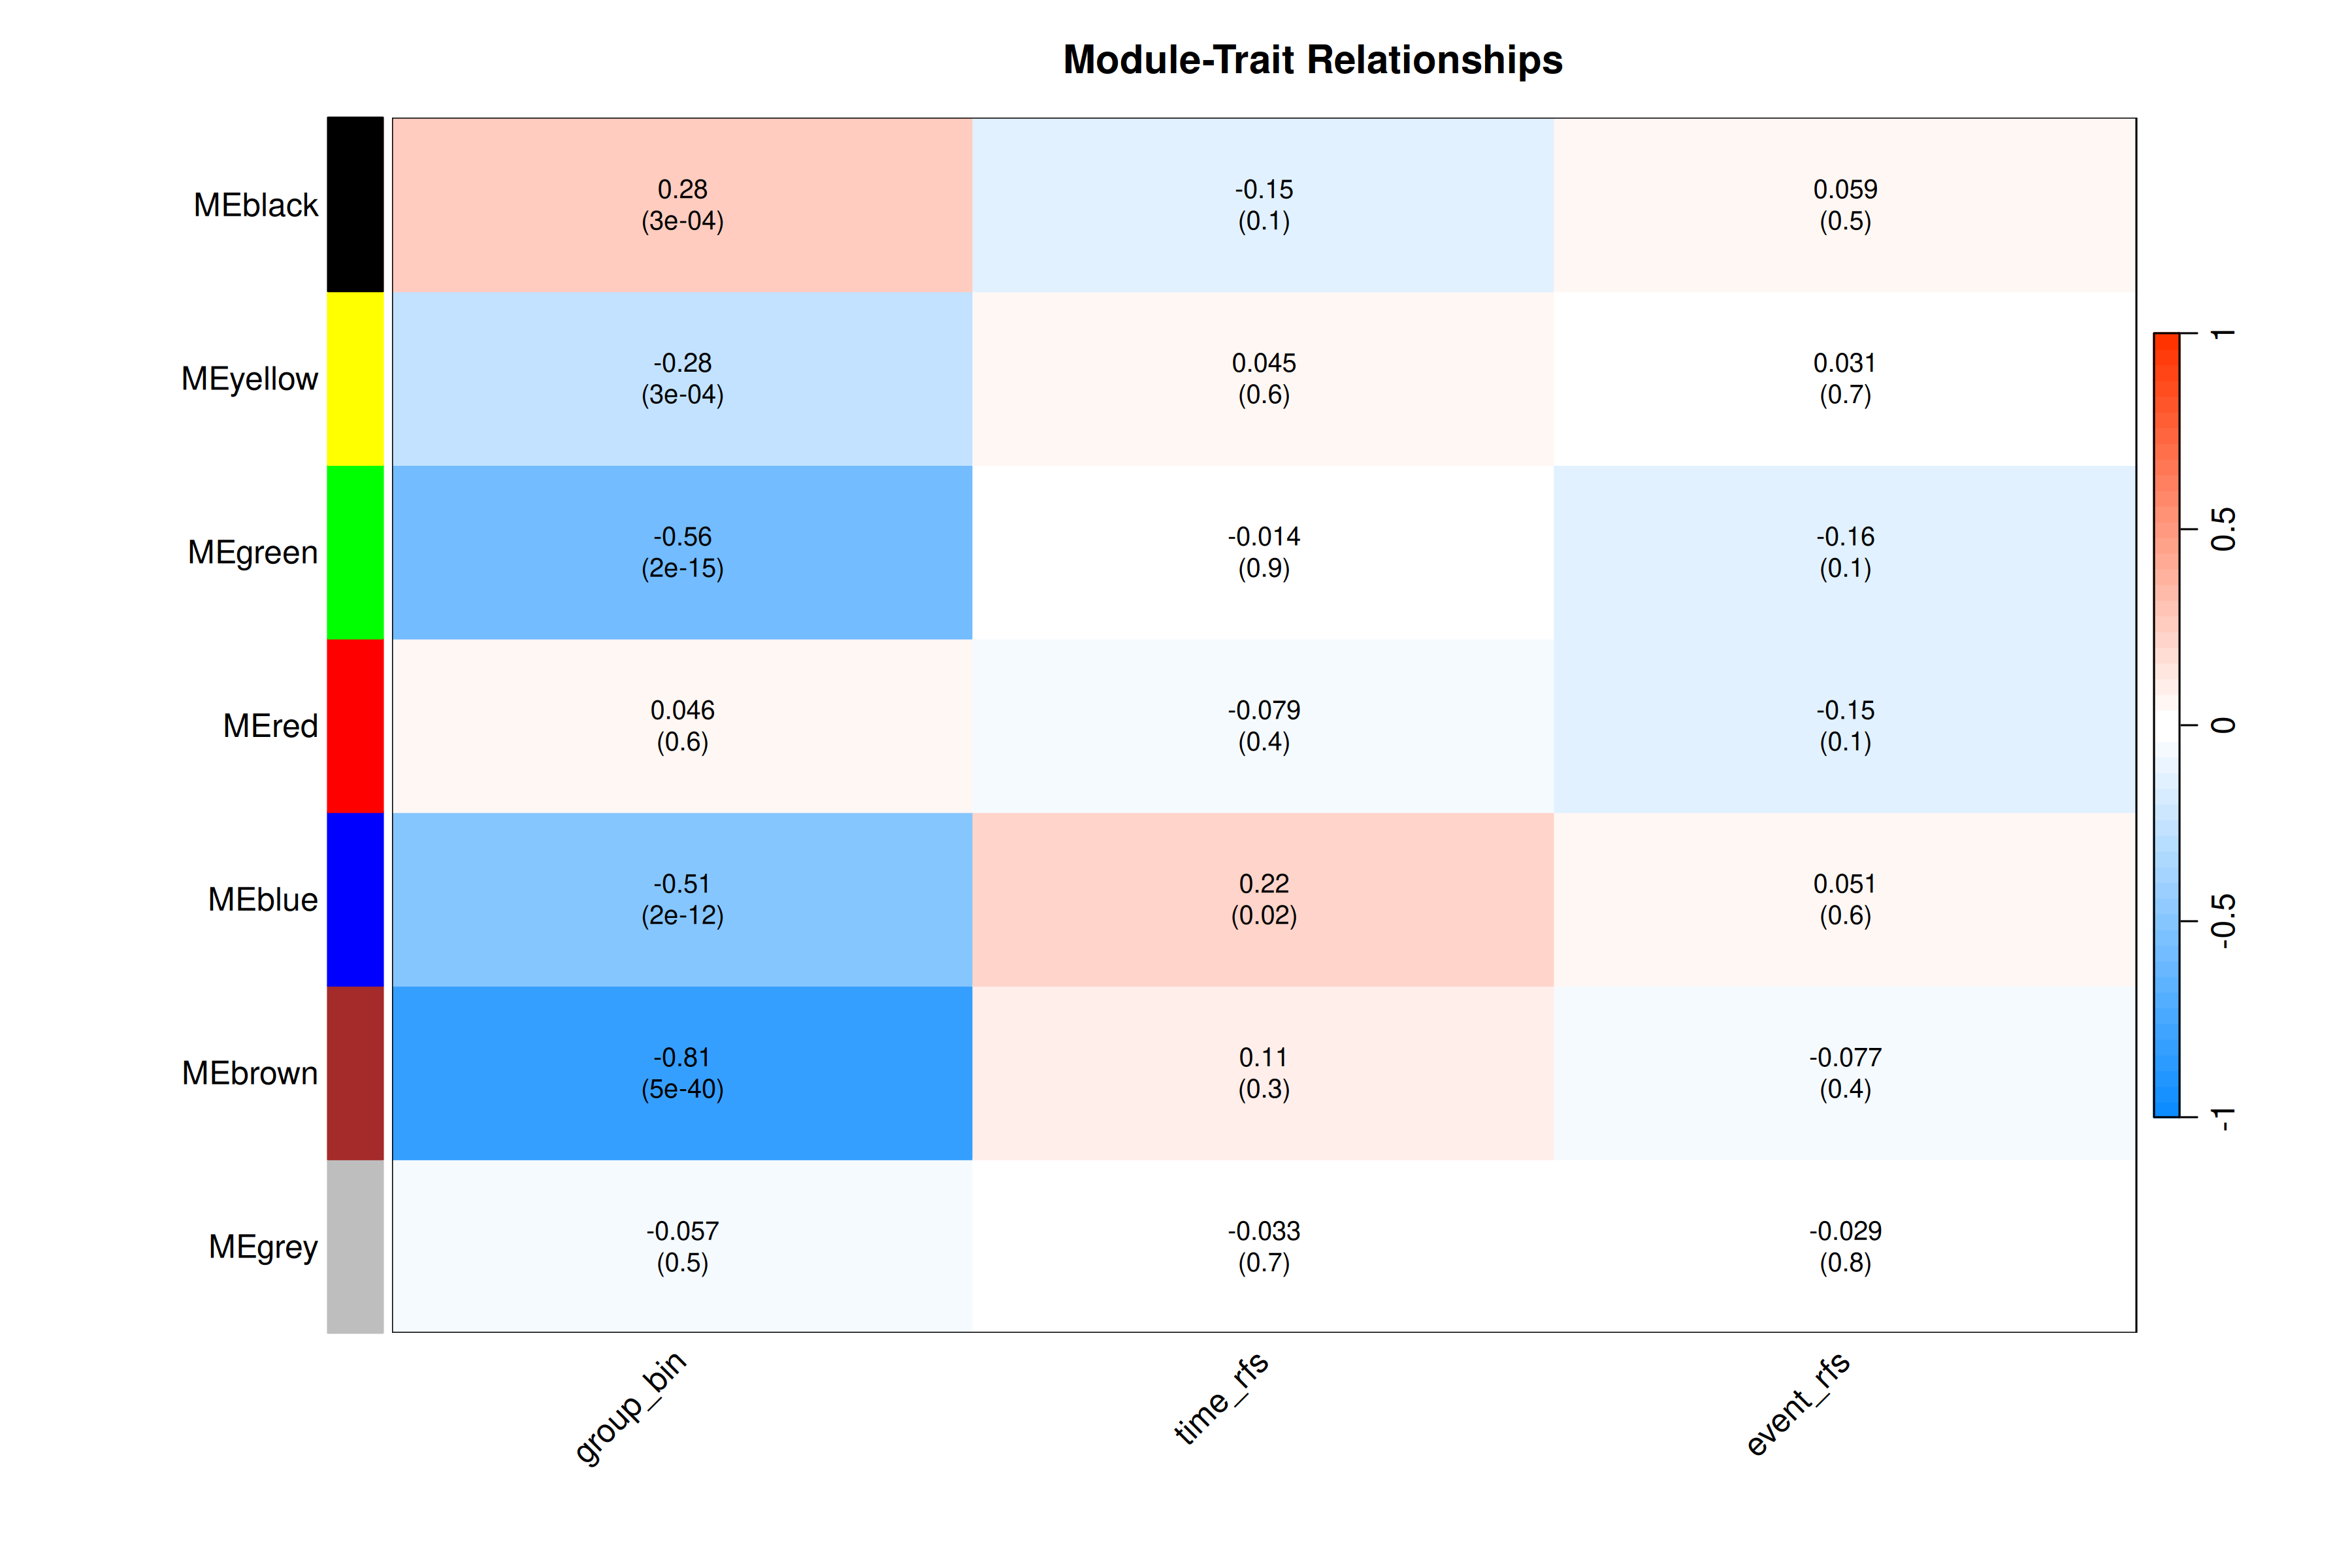
\includegraphics[width=0.8\textwidth]{module_trait_heatmap.png}
\caption{Modül-Trait ilişki ısı haritası}
\label{fig:modtrait}
\end{figure}

\section{Hub Genler}

Hub genler, her modül içinde merkeze yakın ve tümör/non-tümör ayrımıyla güçlü ilişki gösteren genler arasından seçilmiştir. Bu seçimde modül üyeliği (kME) ve gen anlamlılığı (GS) değerleri dikkate alınmıştır.

Brown modülüne ait seçilen hub genler Tablo~\ref{tab:hub}'da verilmiştir. Bu modül için kME-GS dağılımı Şekil~\ref{fig:mmgs}'de, hub genler etrafında oluşturulan co-expression ağı ise Şekil~\ref{fig:network}'te gösterilmiştir.

\begin{table}[H]
\centering
\caption{Brown modülü hub genleri}
\label{tab:hub}
\begin{tabularx}{\textwidth}{lrrX}
\toprule
\textbf{Gen} & \textbf{kME} & \textbf{GS} & \textbf{Fonksiyon} \\
\midrule
GLYATL1 & 0,92 & 0,70 & Glisin konjugasyonu, karaciğer detoksifikasyonu \\
TTC36 & 0,92 & 0,82 & p53 stabilizasyonu \\
PEX11G & 0,90 & 0,69 & Peroksizomal bölünme, lipid metabolizması \\
AADAT & 0,90 & 0,80 & Kinürenin yolağı, amino asit metabolizması \\
NAT2 & 0,89 & 0,77 & N-asetiltransferaz, ilaç metabolizması \\
\bottomrule
\end{tabularx}
\end{table}

\begin{figure}[H]
\centering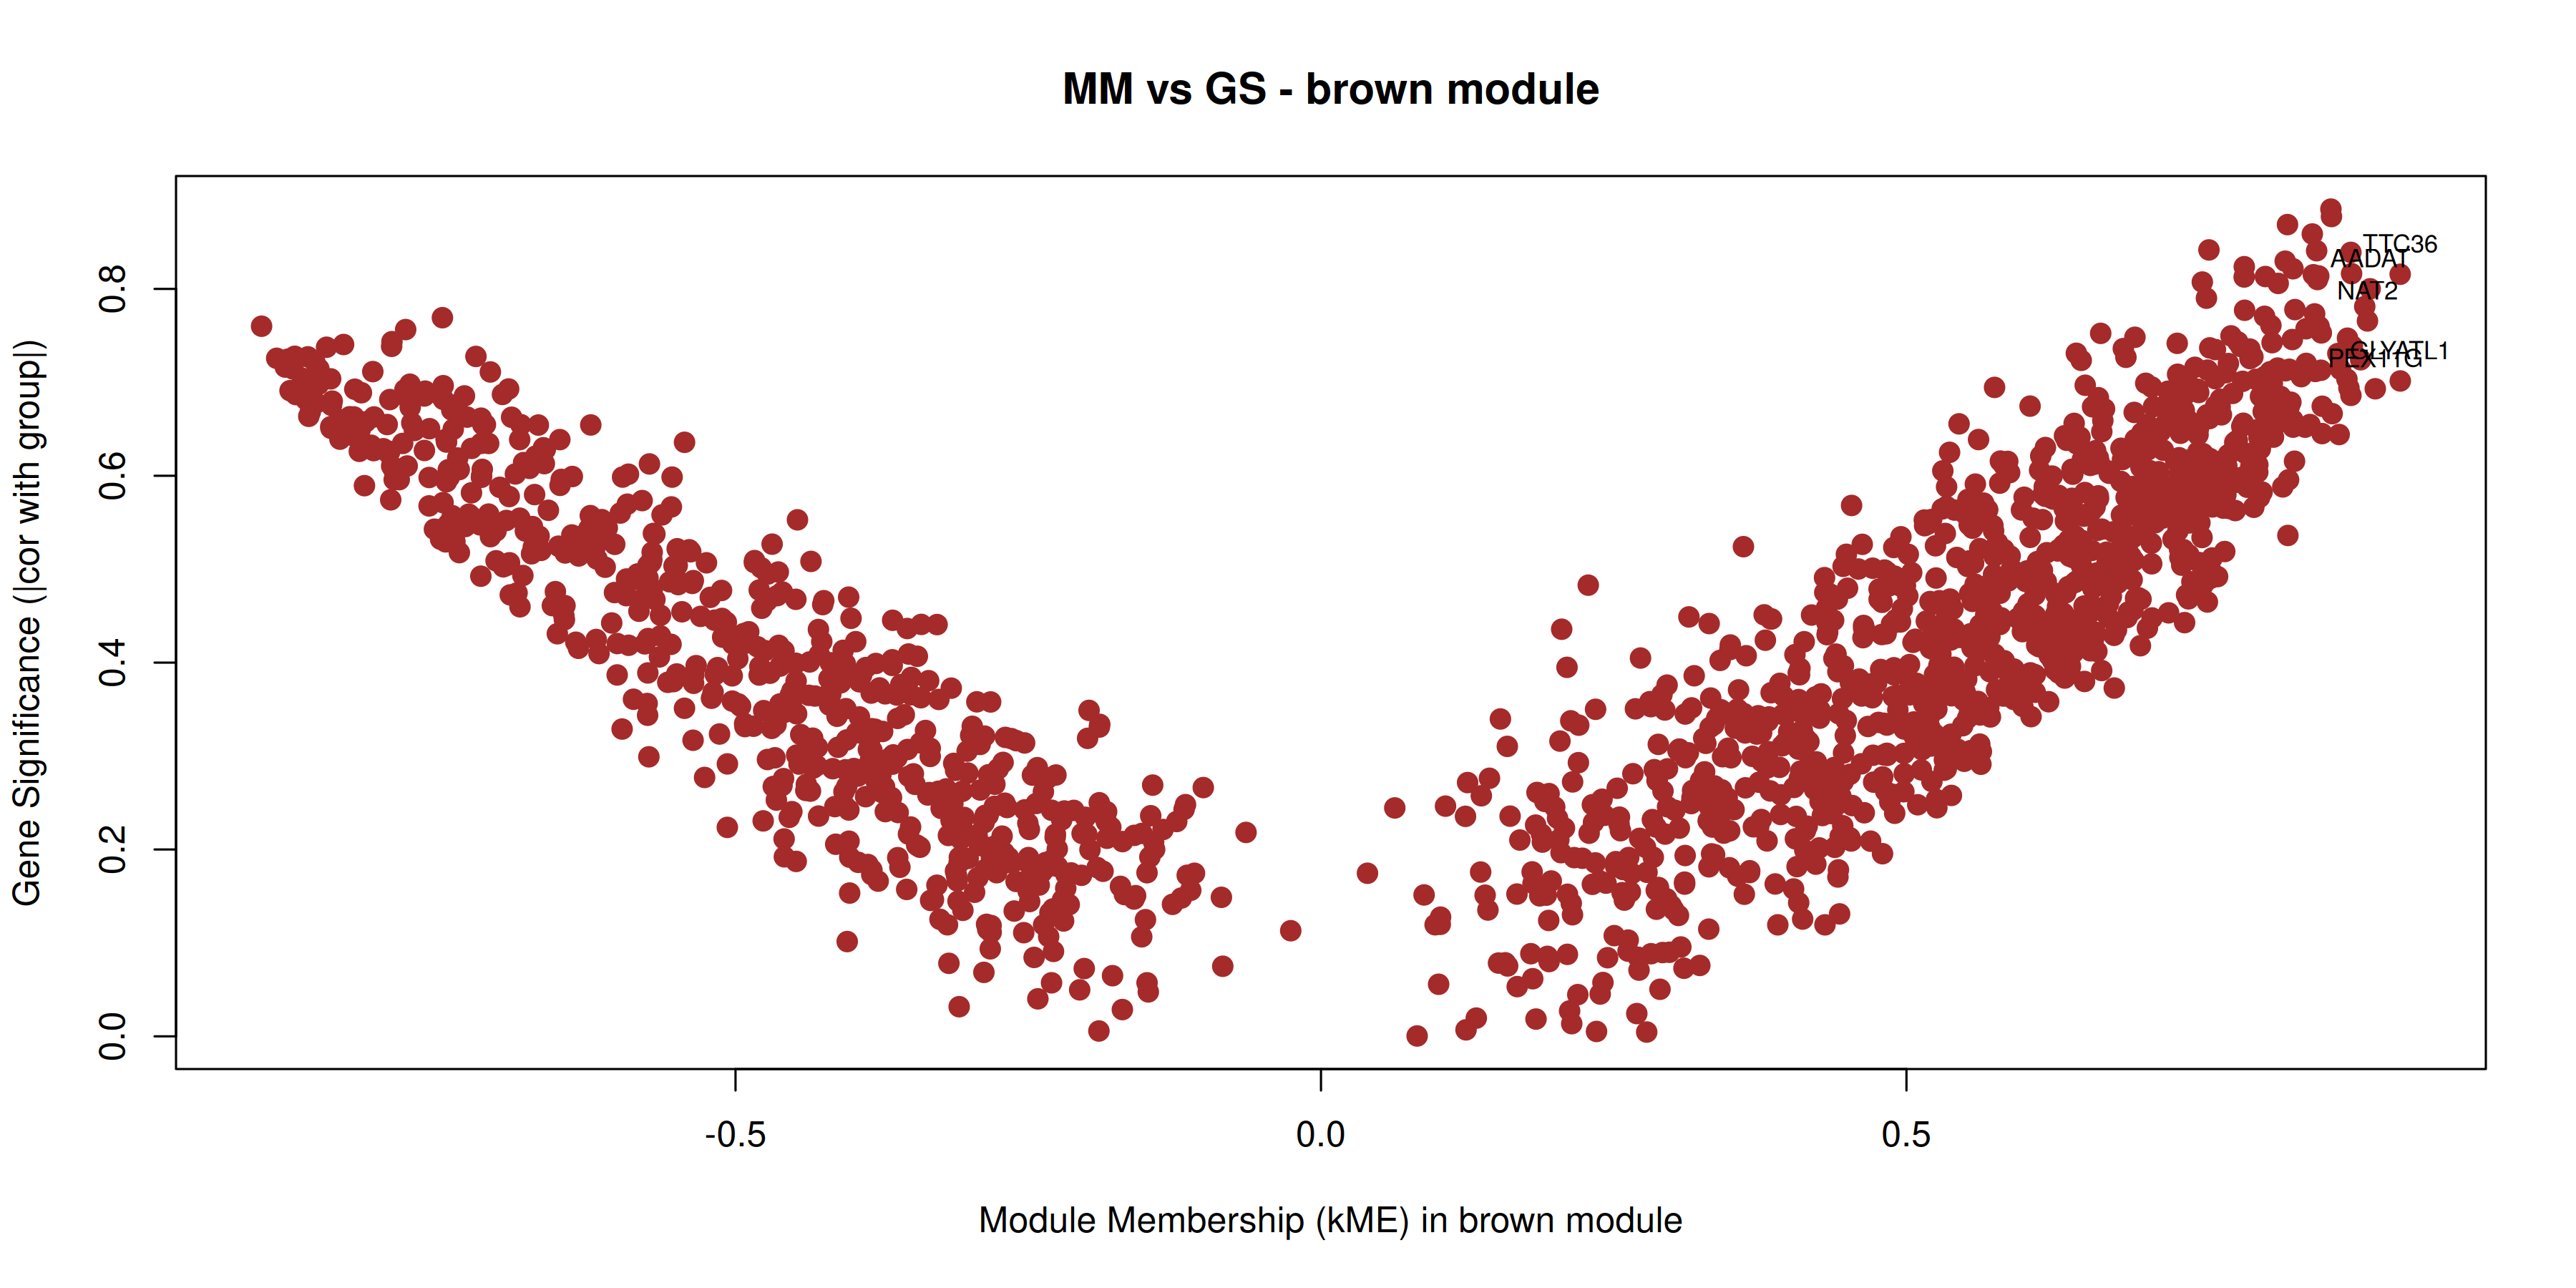
\includegraphics[width=0.9\textwidth]{mm_vs_gs_brown.png}
\caption{Brown modülü için Module Membership (MM) - Gene Significance (GS) dağılımı}
\label{fig:mmgs}
\end{figure}

\begin{figure}[H]
\centering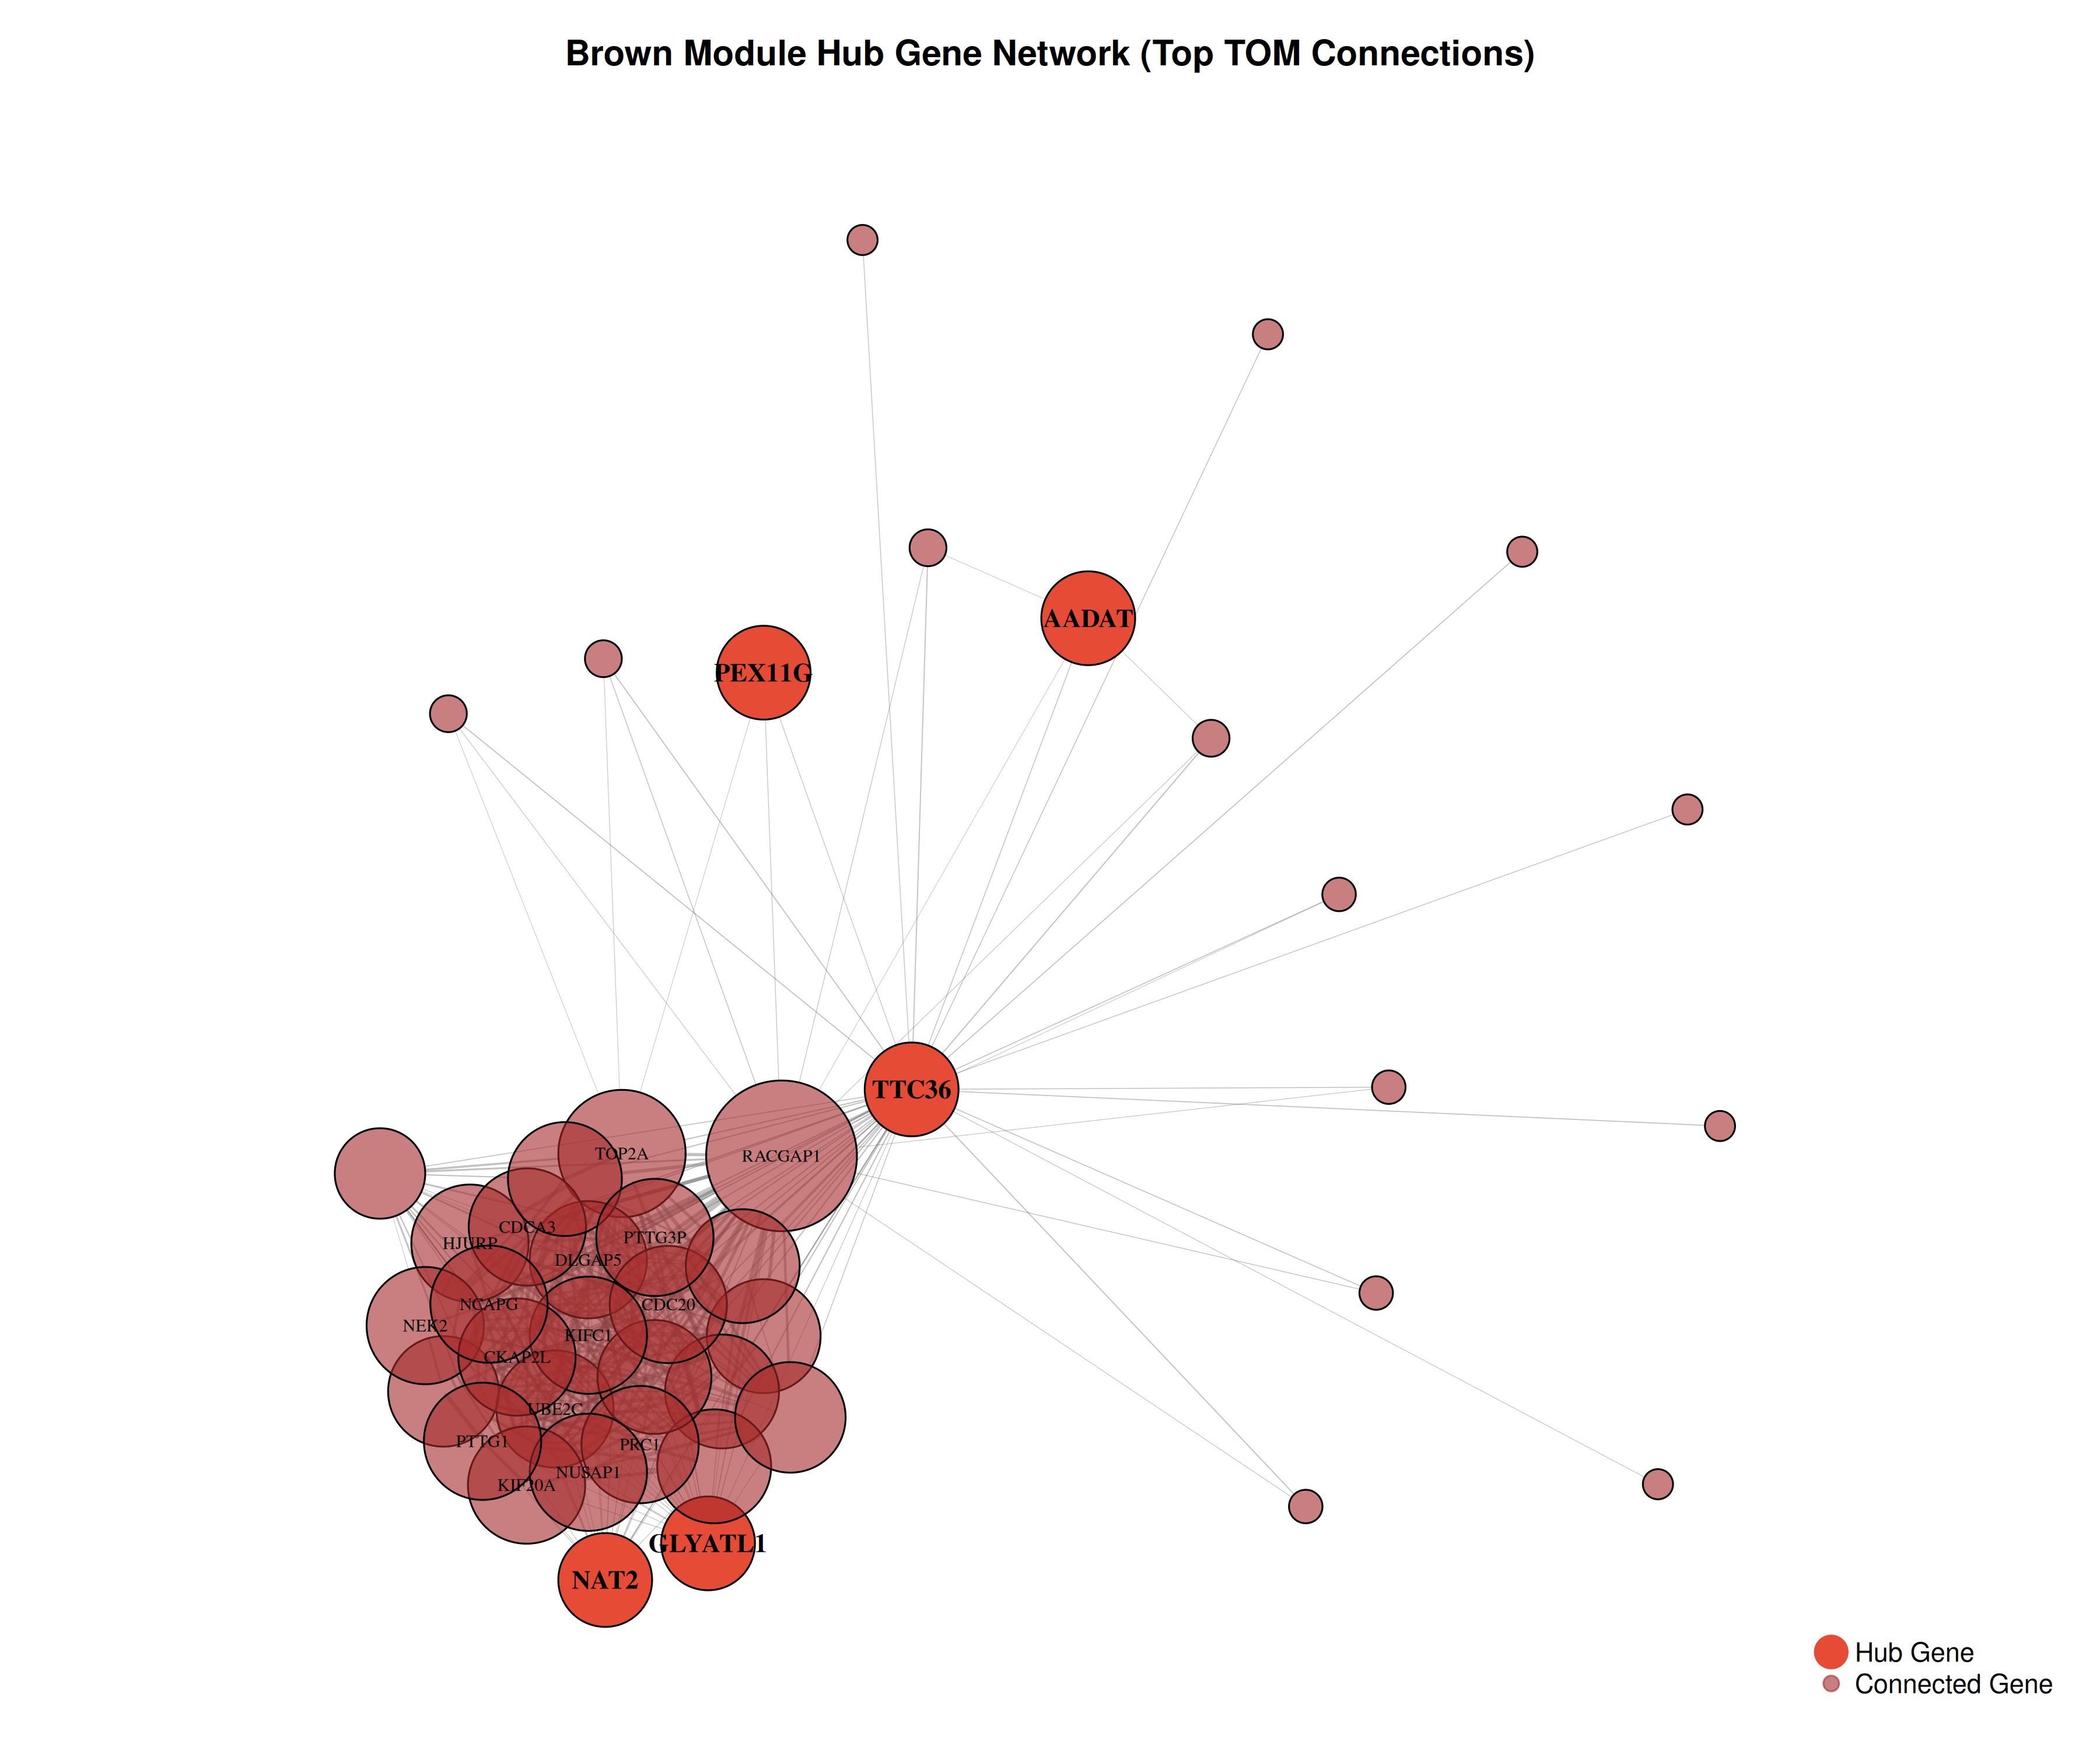
\includegraphics[width=0.95\textwidth]{network_brown_module.png}
\caption{Brown modülü hub gen merkezli co-expression ağı}
\label{fig:network}
\end{figure}

% ------------------------------------------------------------------------------
\chapter{GO ENRICHMENT ANALİZİ}

\section{Yöntem}

Brown modülünde yer alan 1636 gen için GO enrichment analizi yapılmıştır. Bu analizde, genlerin hangi biyolojik süreçlerle daha fazla ilişkili olduğunu belirlemek amaçlanmıştır.

Analiz sonucunda elde edilen p-değerleri Benjamini-Hochberg yöntemi ile düzeltilmiş ve anlamlı GO terimleri belirlenmiştir.

\section{Sonuçlar}

Brown modülü için 752 anlamlı Biyolojik Süreç terimi tespit edilmiştir. En anlamlı terimler Tablo~\ref{tab:go} içinde verilmiştir. Sonuçlar bar grafiği (Şekil~\ref{fig:gobar}) ve nokta grafiği (Şekil~\ref{fig:godot}) ile görselleştirilmiştir.

\begin{table}[H]
\centering
\caption{En anlamlı GO Biyolojik Süreç terimleri}
\label{tab:go}
\begin{tabularx}{\textwidth}{X r r}
\toprule
\textbf{GO Terimi} & \textbf{p.adjust} & \textbf{Gen Sayısı} \\
\midrule
Small molecule catabolic process & $3{,}85\times10^{-54}$ & 138 \\
Organic acid catabolic process & $8{,}60\times10^{-50}$ & 108 \\
Carboxylic acid catabolic process & $8{,}60\times10^{-50}$ & 108 \\
Alpha-amino acid metabolic process & $4{,}60\times10^{-36}$ & 84 \\
Organic acid biosynthetic process & $8{,}77\times10^{-36}$ & 108 \\
Amino acid metabolic process & $4{,}44\times10^{-32}$ & 95 \\
Fatty acid metabolic process & $7{,}55\times10^{-30}$ & 110 \\
\bottomrule
\end{tabularx}
\end{table}

\begin{figure}[H]
\centering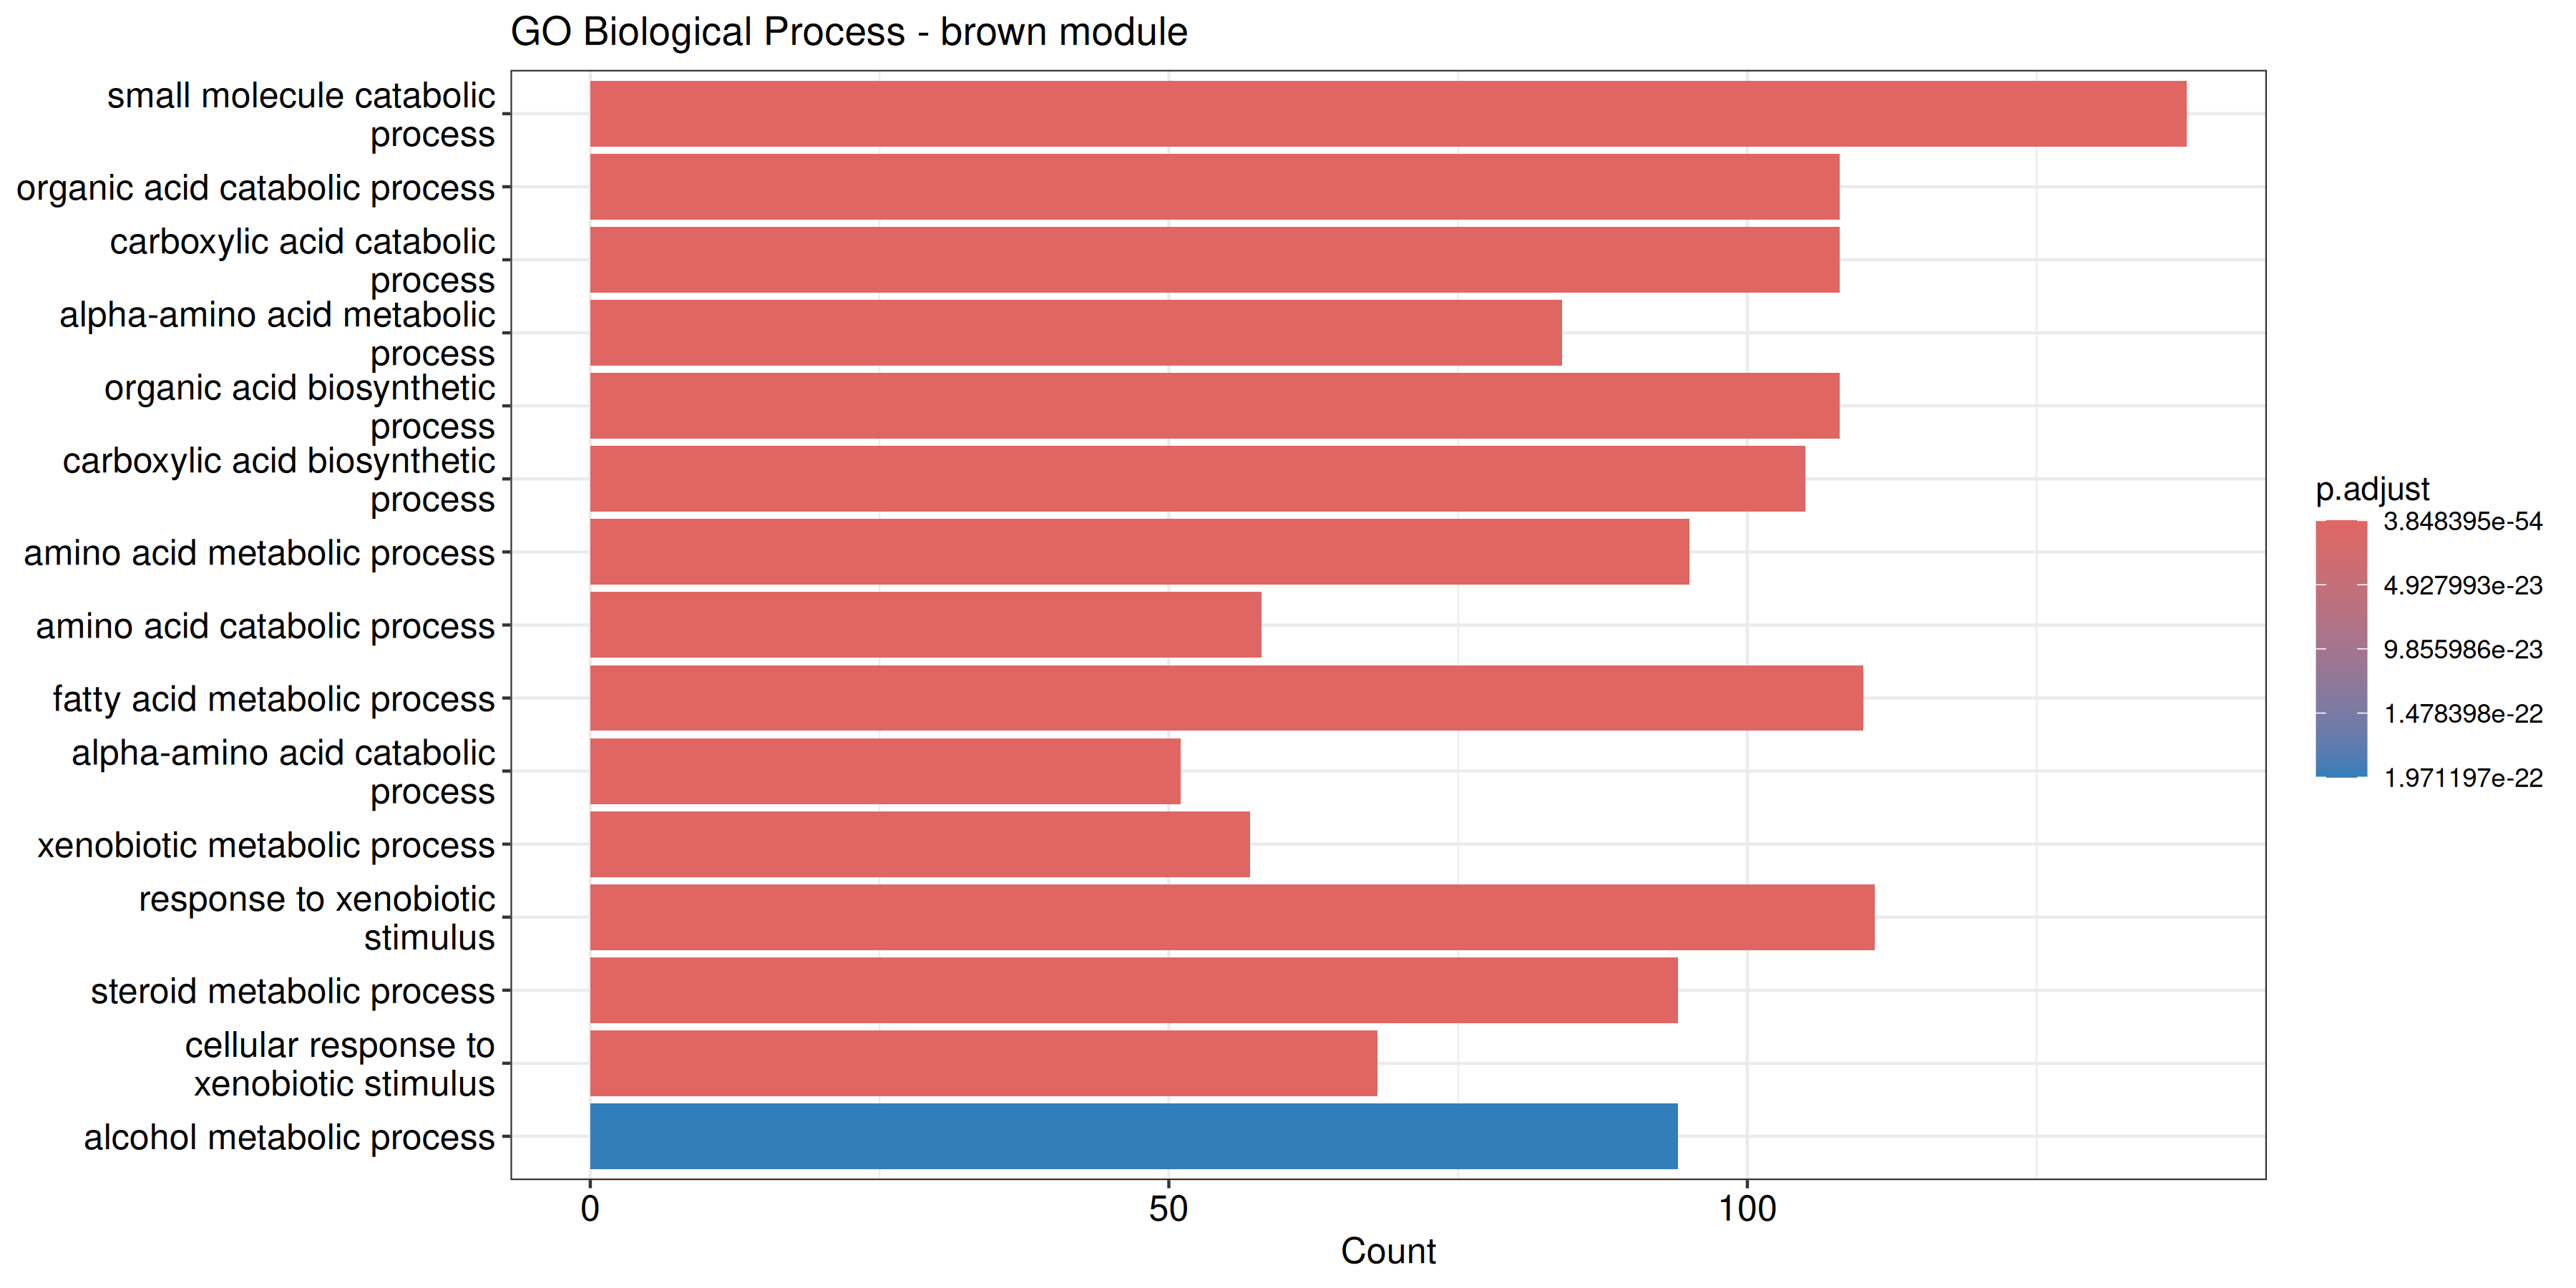
\includegraphics[width=0.95\textwidth]{go_barplot.png}
\caption{GO Biyolojik Süreç bar grafiği}
\label{fig:gobar}
\end{figure}

\begin{figure}[H]
\centering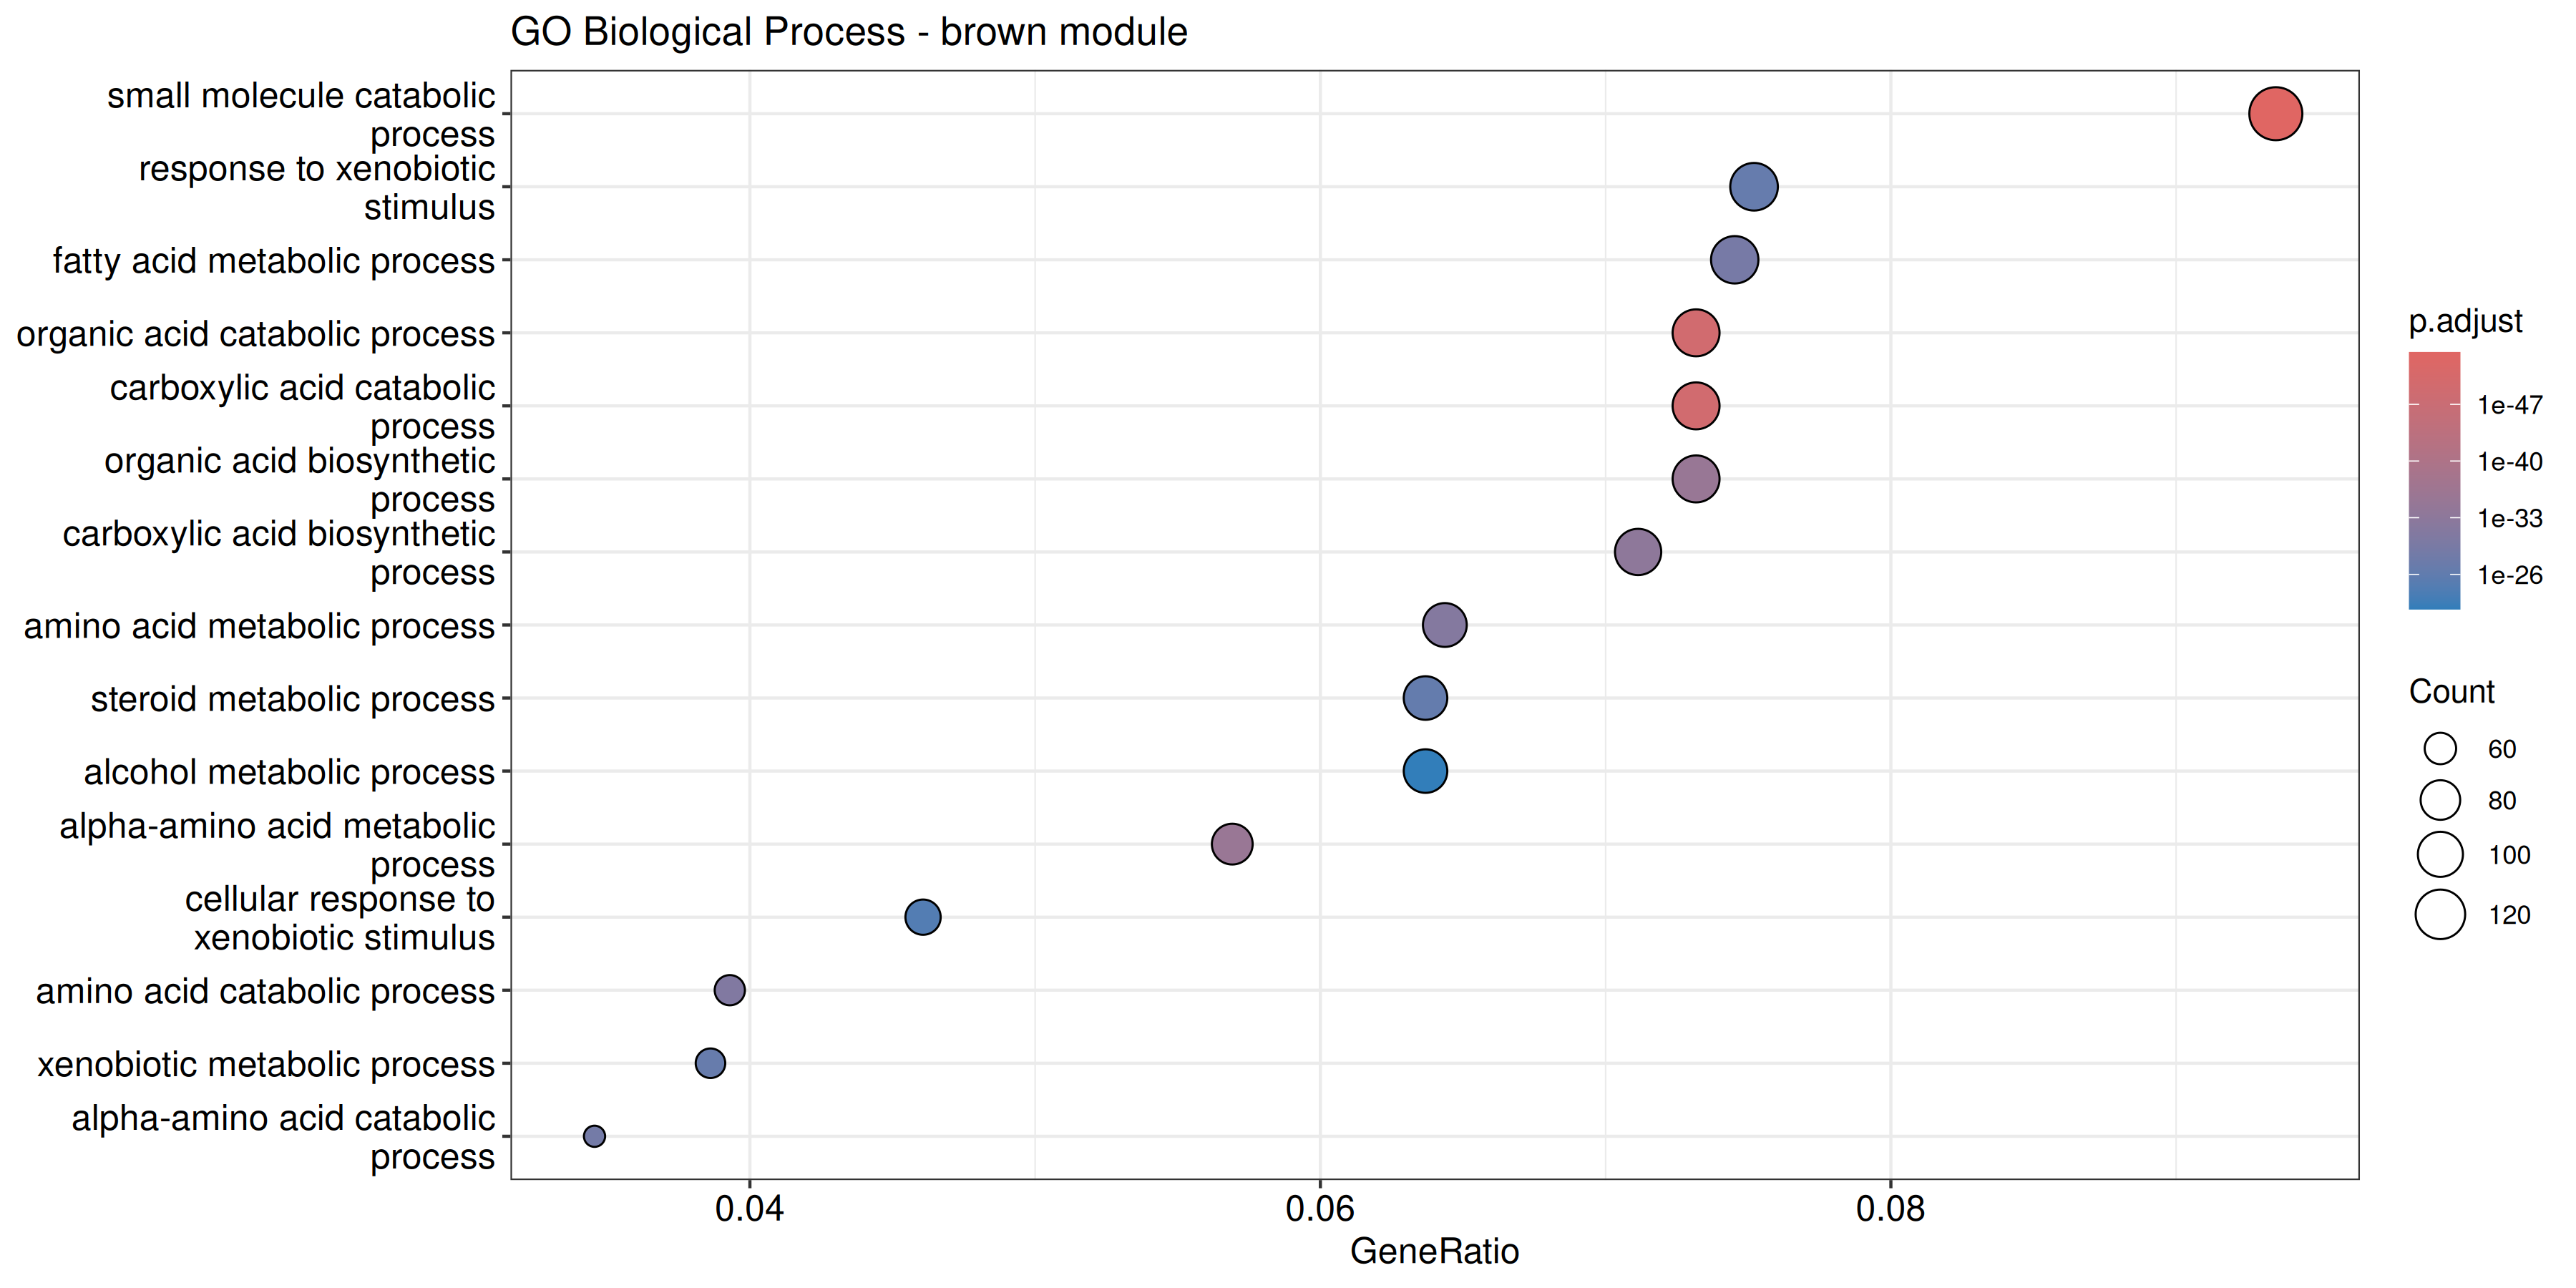
\includegraphics[width=0.95\textwidth]{go_dotplot.png}
\caption{GO Biyolojik Süreç nokta grafiği}
\label{fig:godot}
\end{figure}

\section{Biyolojik Yorum}

En anlamlı GO terimleri küçük molekül yıkımı, amino asit metabolizması ve yağ asidi metabolizması ile ilişkilidir. Bu süreçler karaciğerin temel görevleri arasında yer almaktadır.

Brown modülünün tümör örnekleriyle negatif ilişki göstermesi, HCC dokusunda normal karaciğer metabolizmasıyla ilişkili genlerin daha düşük ifade edildiğini düşündürmektedir. Bu sonuç, tümör dokusunda metabolik kapasitenin azalabileceği yorumunu desteklemektedir.

% ------------------------------------------------------------------------------
\chapter{MAKİNE ÖĞRENMESİ İLE SINIFLANDIRMA}

\section{Özellik Seçimi/Çıkarımı Setup'ları}

Tümör/non-tümör sınıflandırması için üç farklı özellik stratejisi karşılaştırılmıştır (Tablo~\ref{tab:setups}).

\begin{table}[H]
\centering
\caption{Özellik seçimi/çıkarımı setup'ları}
\label{tab:setups}
\begin{tabularx}{\textwidth}{l l X}
\toprule
\textbf{Özellik Seti} & \textbf{Özellik Sayısı} & \textbf{Yöntem} \\
\midrule
Biyolojik & 742 gen & DGE sonucunda bulunan anlamlı genler ve WGCNA hub genleri \\
İstatistiksel & 446 gen & Yüksek varyanslı ve birbirine çok benzemeyen genler \\
PCA & 35 bileşen & Gen ifade verilerinin PCA ile özetlenmiş hali (\%80 varyans) \\
\bottomrule
\end{tabularx}
\end{table}

\section{Modeller ve Değerlendirme}

Üç farklı eğiticili makine öğrenmesi modeli kullanılmıştır: SVM, Random Forest ve XGBoost. Modeller, çapraz doğrulama ile değerlendirilmiştir. Bu yöntemde aynı hastaya ait tümör ve non-tümör örnekleri aynı katta tutulmuş, böylece aynı hastadan gelen örneklerin hem eğitim hem test verisine düşmesi engellenmiştir.

Sınıflandırmada pozitif sınıf Tümör olarak belirlenmiştir. PCA kullanılan Setup-3'te, boyut indirgeme işlemi her çapraz doğrulama katında yalnızca eğitim verisi üzerinde öğrenilmiştir. Böylece test verisinden modele bilgi sızması önlenmiştir.

Model başarısı Accuracy, Precision, Recall, F1 ve AUC metrikleriyle değerlendirilmiştir.

\section{Sonuçlar}

Üç farklı özellik seti ve üç farklı model için elde edilen sonuçlar Tablo~\ref{tab:ml} içinde verilmiştir. Tüm modeller \%93 üzeri accuracy ve 0,95 üzeri AUC değeri elde etmiştir.

\begin{table}[H]
\centering
\caption{Makine öğrenmesi model karşılaştırması (kalın değerler sütun bazındaki en iyi değerleri gösterir)}
\label{tab:ml}
\begin{tabular}{llrrrrr}
\toprule
\textbf{Özellik Seti} & \textbf{Model} & \textbf{Acc} & \textbf{Prec} & \textbf{Recall} & \textbf{F1} & \textbf{AUC} \\
\midrule
Biyolojik & SVM & 0,946 & 0,965 & 0,957 & 0,961 & 0,975 \\
Biyolojik & Random Forest & \textbf{0,958} & 0,974 & 0,965 & 0,969 & 0,980 \\
Biyolojik & XGBoost & 0,952 & 0,965 & 0,965 & 0,965 & 0,973 \\
İstatistiksel & SVM & 0,946 & 0,965 & 0,957 & 0,961 & 0,962 \\
İstatistiksel & Random Forest & \textbf{0,958} & 0,966 & \textbf{0,974} & \textbf{0,970} & \textbf{0,981} \\
İstatistiksel & XGBoost & 0,946 & 0,957 & 0,965 & 0,961 & 0,968 \\
PCA & SVM & \textbf{0,958} & \textbf{0,982} & 0,957 & 0,969 & 0,967 \\
PCA & Random Forest & 0,934 & 0,956 & 0,948 & 0,952 & 0,973 \\
PCA & XGBoost & 0,934 & 0,956 & 0,948 & 0,952 & 0,959 \\
\bottomrule
\end{tabular}
\end{table}

Model bazlı ROC eğrileri Şekil~\ref{fig:roc1}--\ref{fig:roc3}, örnek karışıklık matrisleri Şekil~\ref{fig:cm} ile verilmiştir.

\begin{figure}[H]
\centering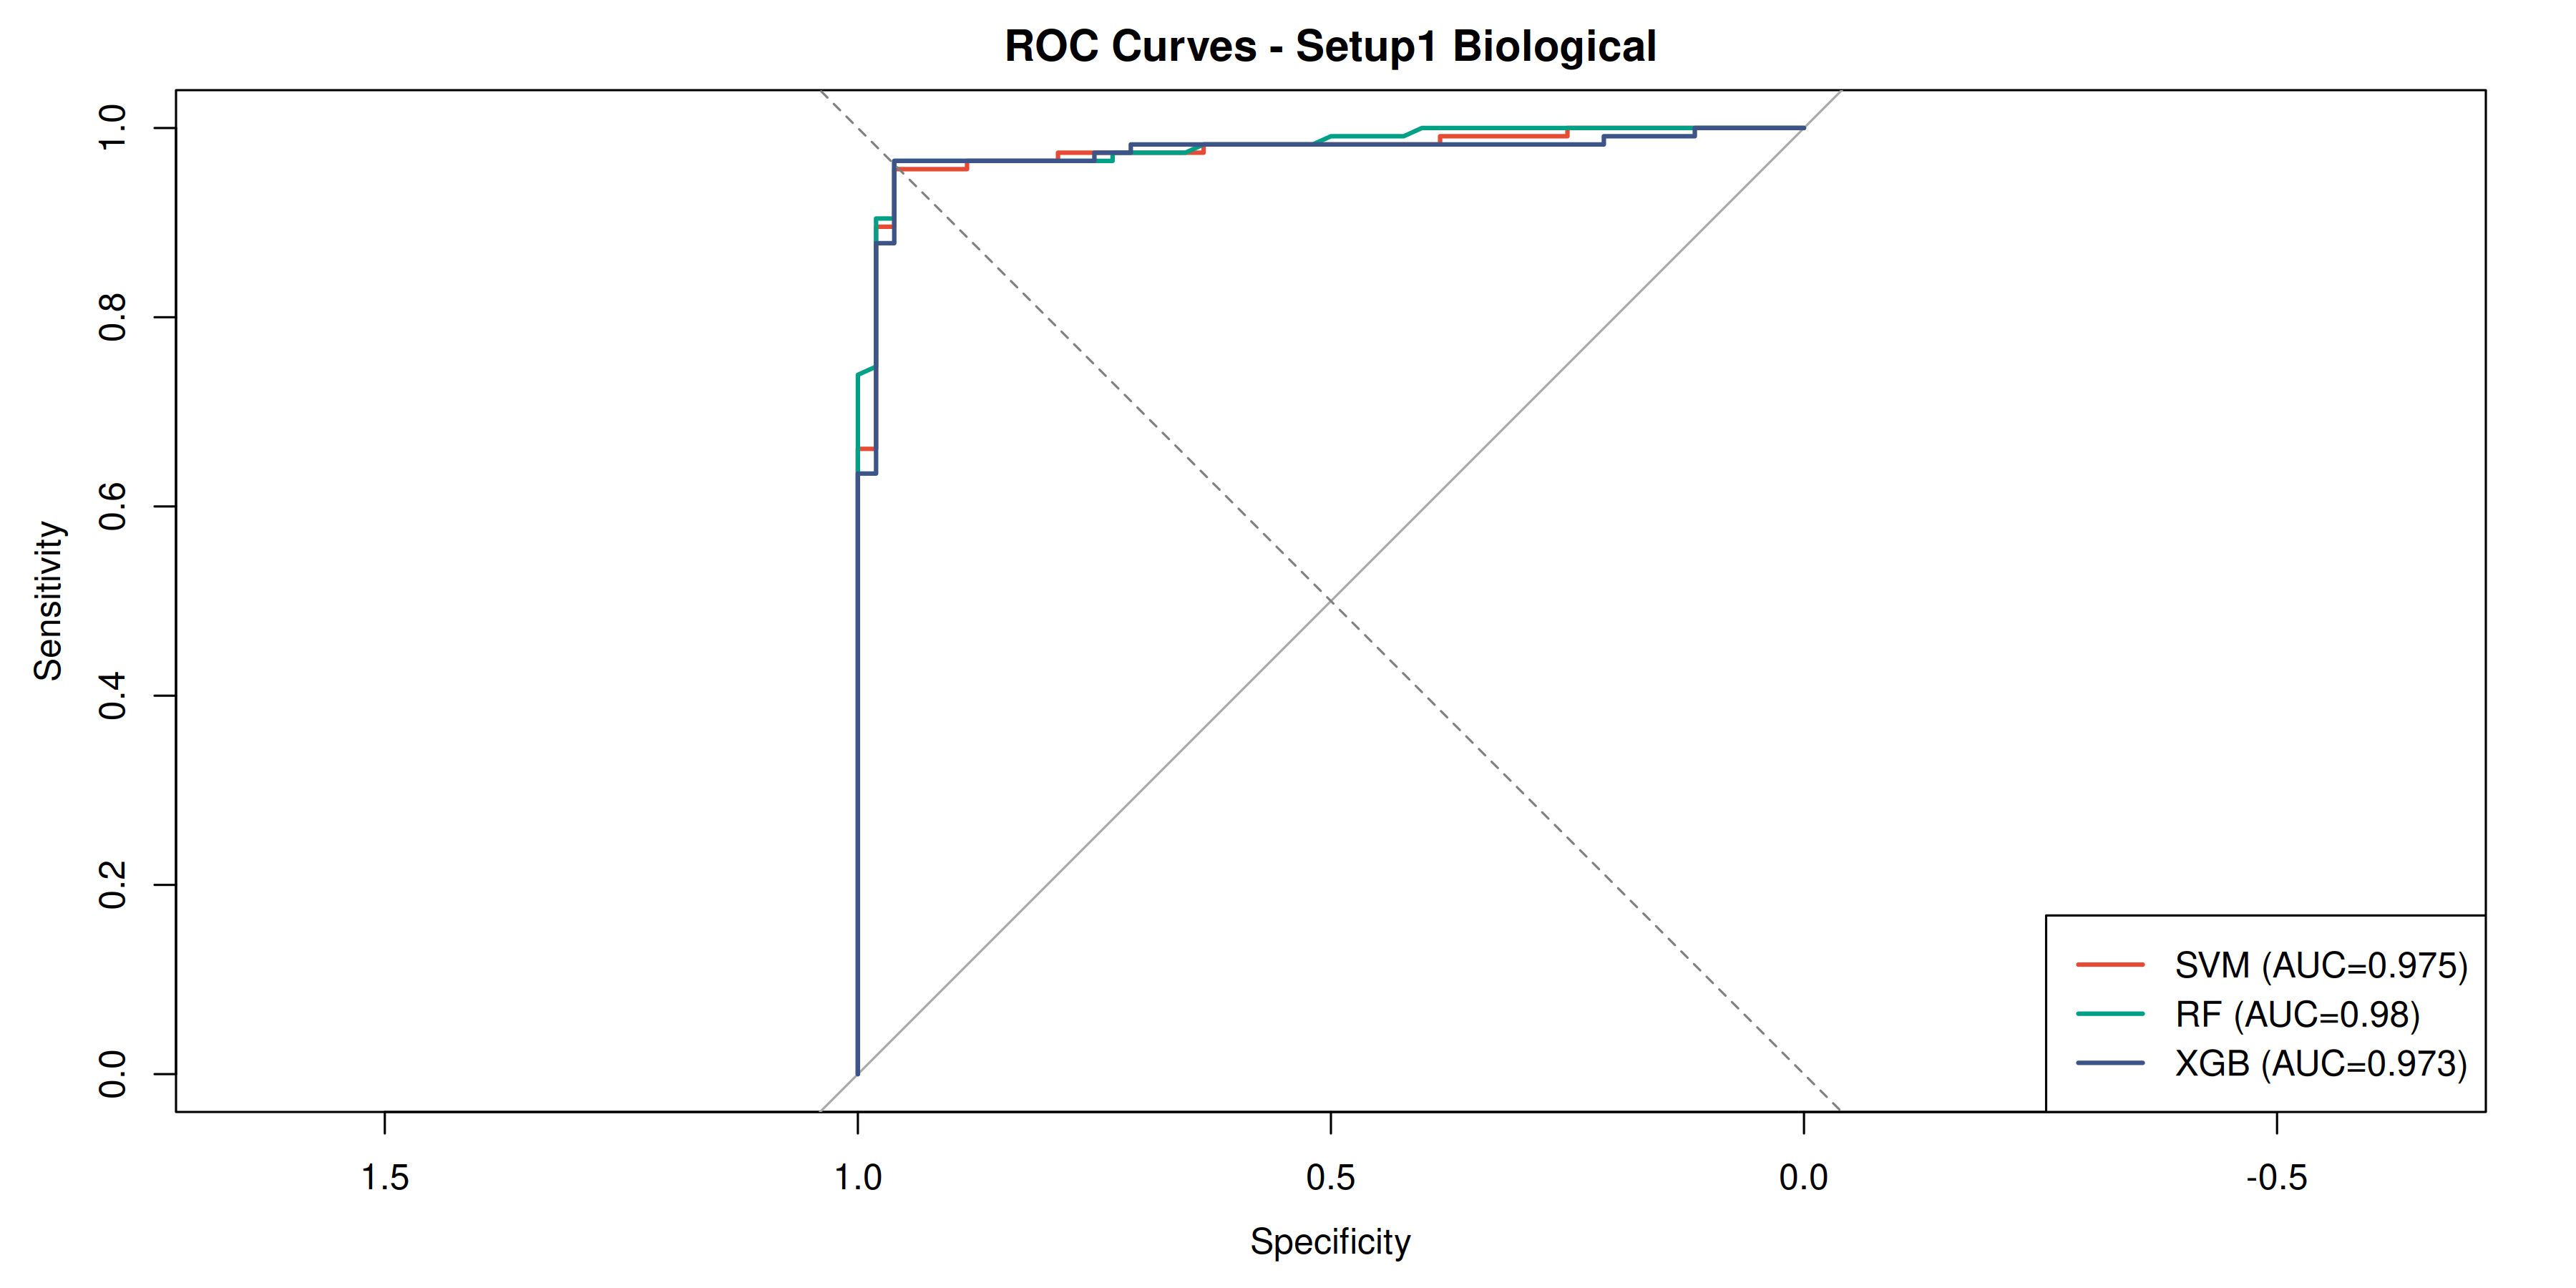
\includegraphics[width=0.85\textwidth]{roc_curves_Setup1_Biological.png}
\caption{Biyolojik ROC eğrileri}
\label{fig:roc1}
\end{figure}

\begin{figure}[H]
\centering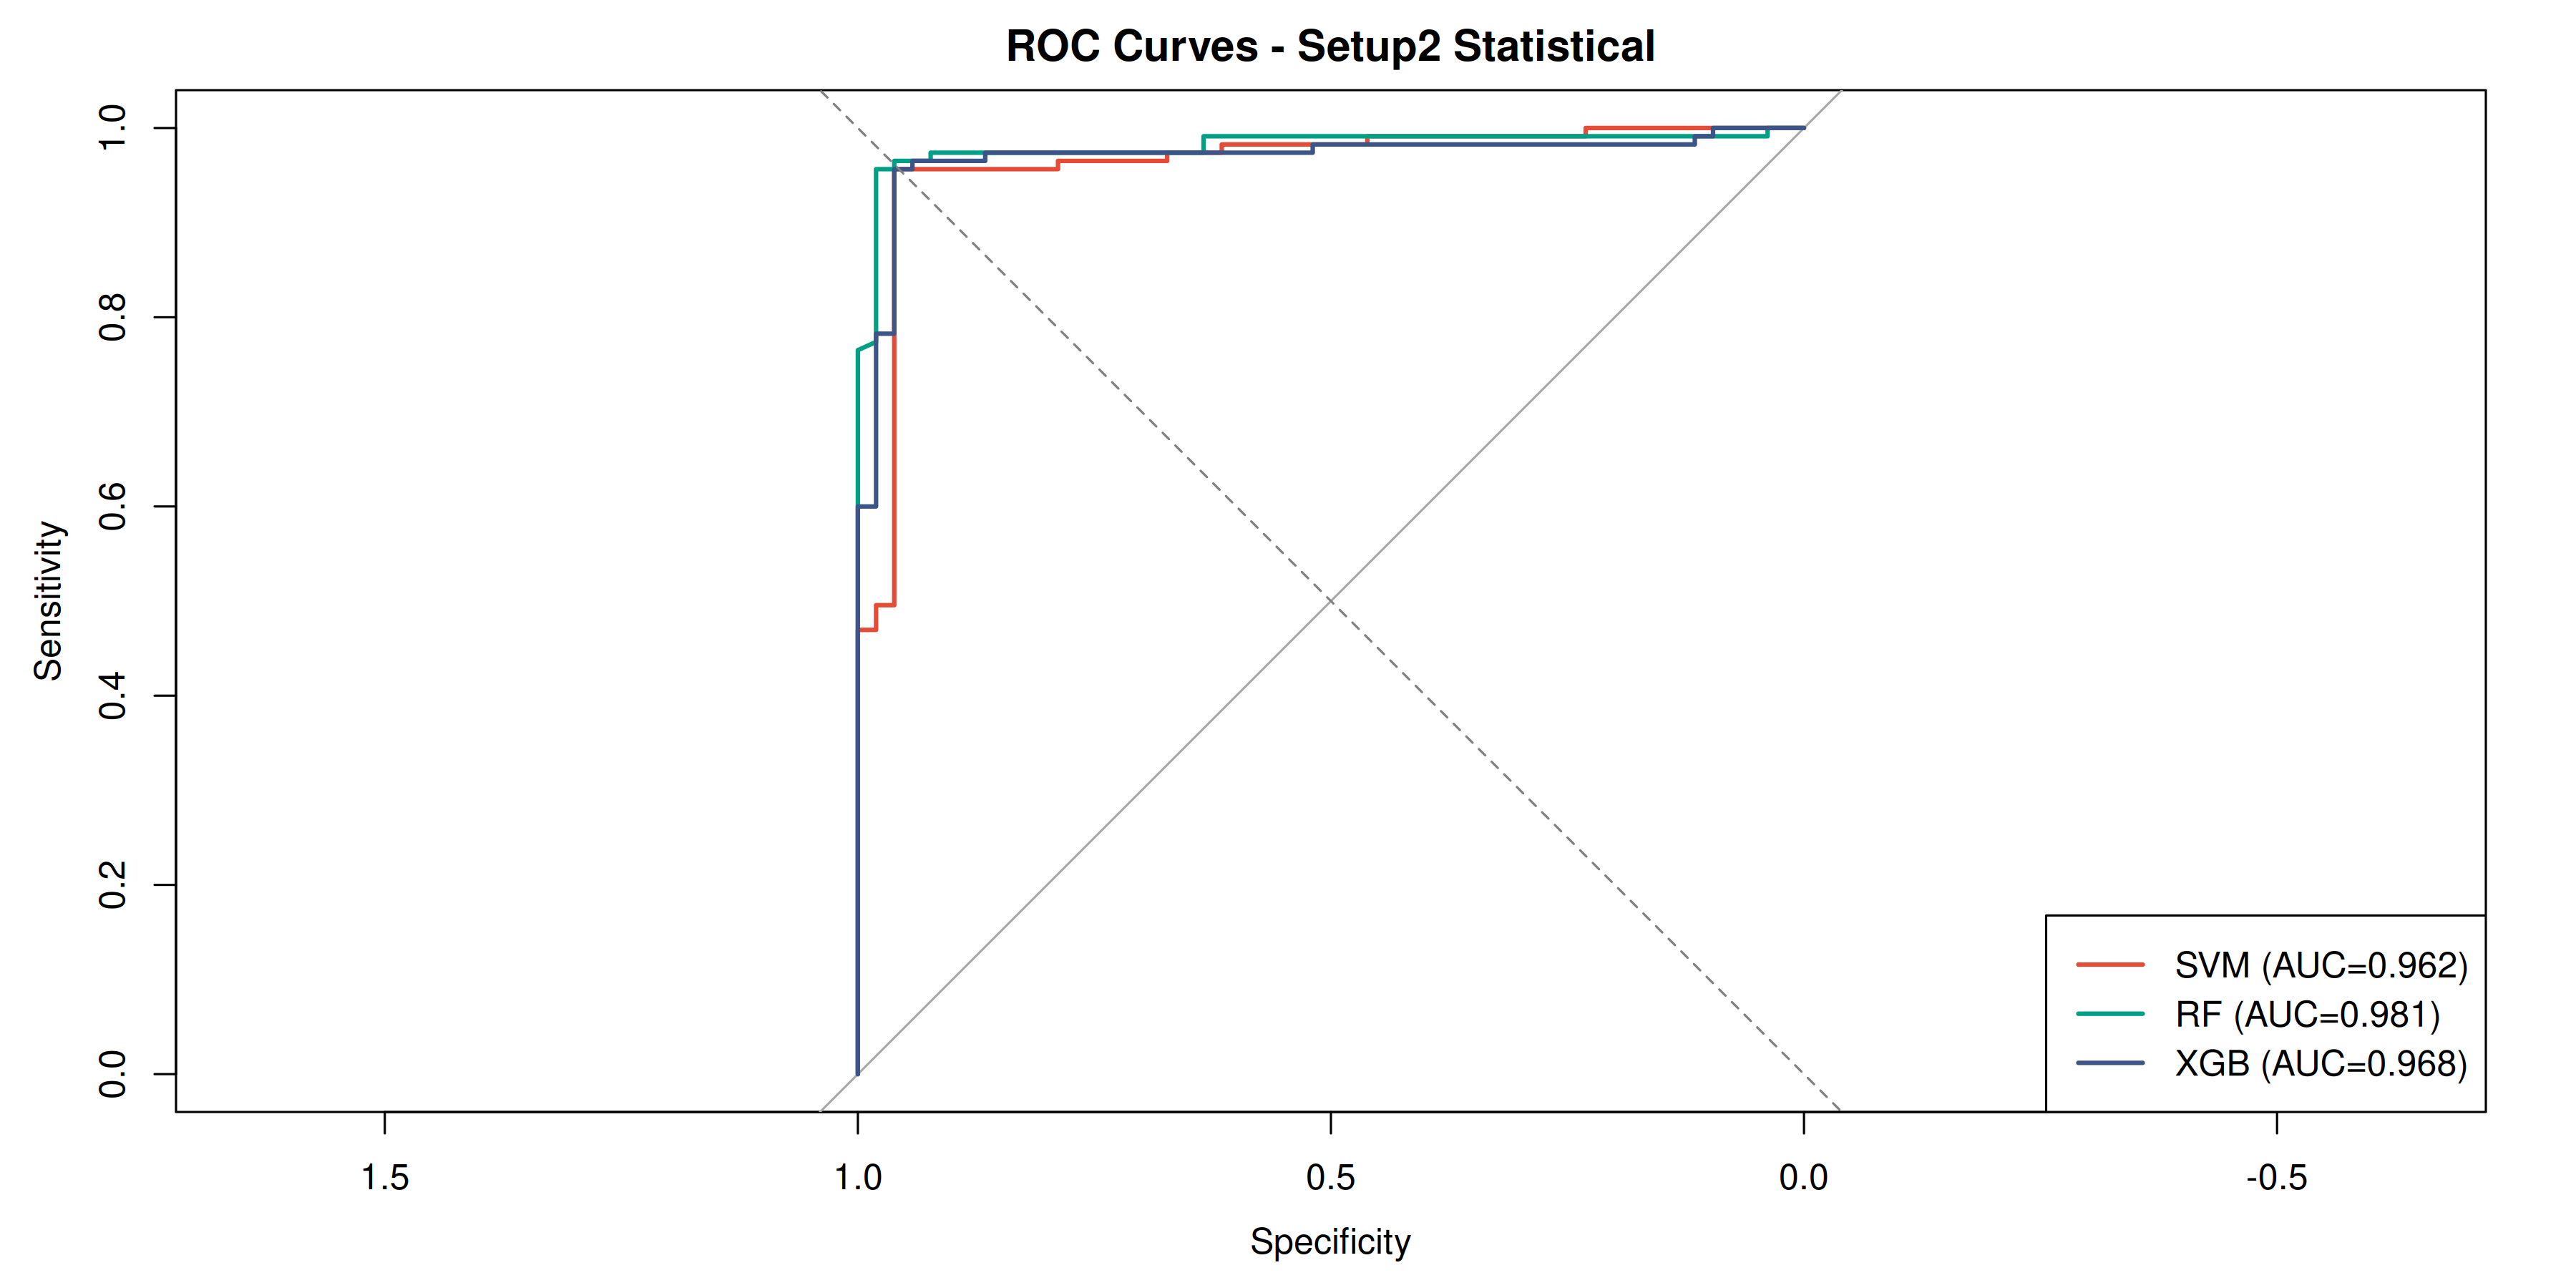
\includegraphics[width=0.85\textwidth]{roc_curves_Setup2_Statistical.png}
\caption{İstatistiksel ROC eğrileri}
\label{fig:roc2}
\end{figure}

\begin{figure}[H]
\centering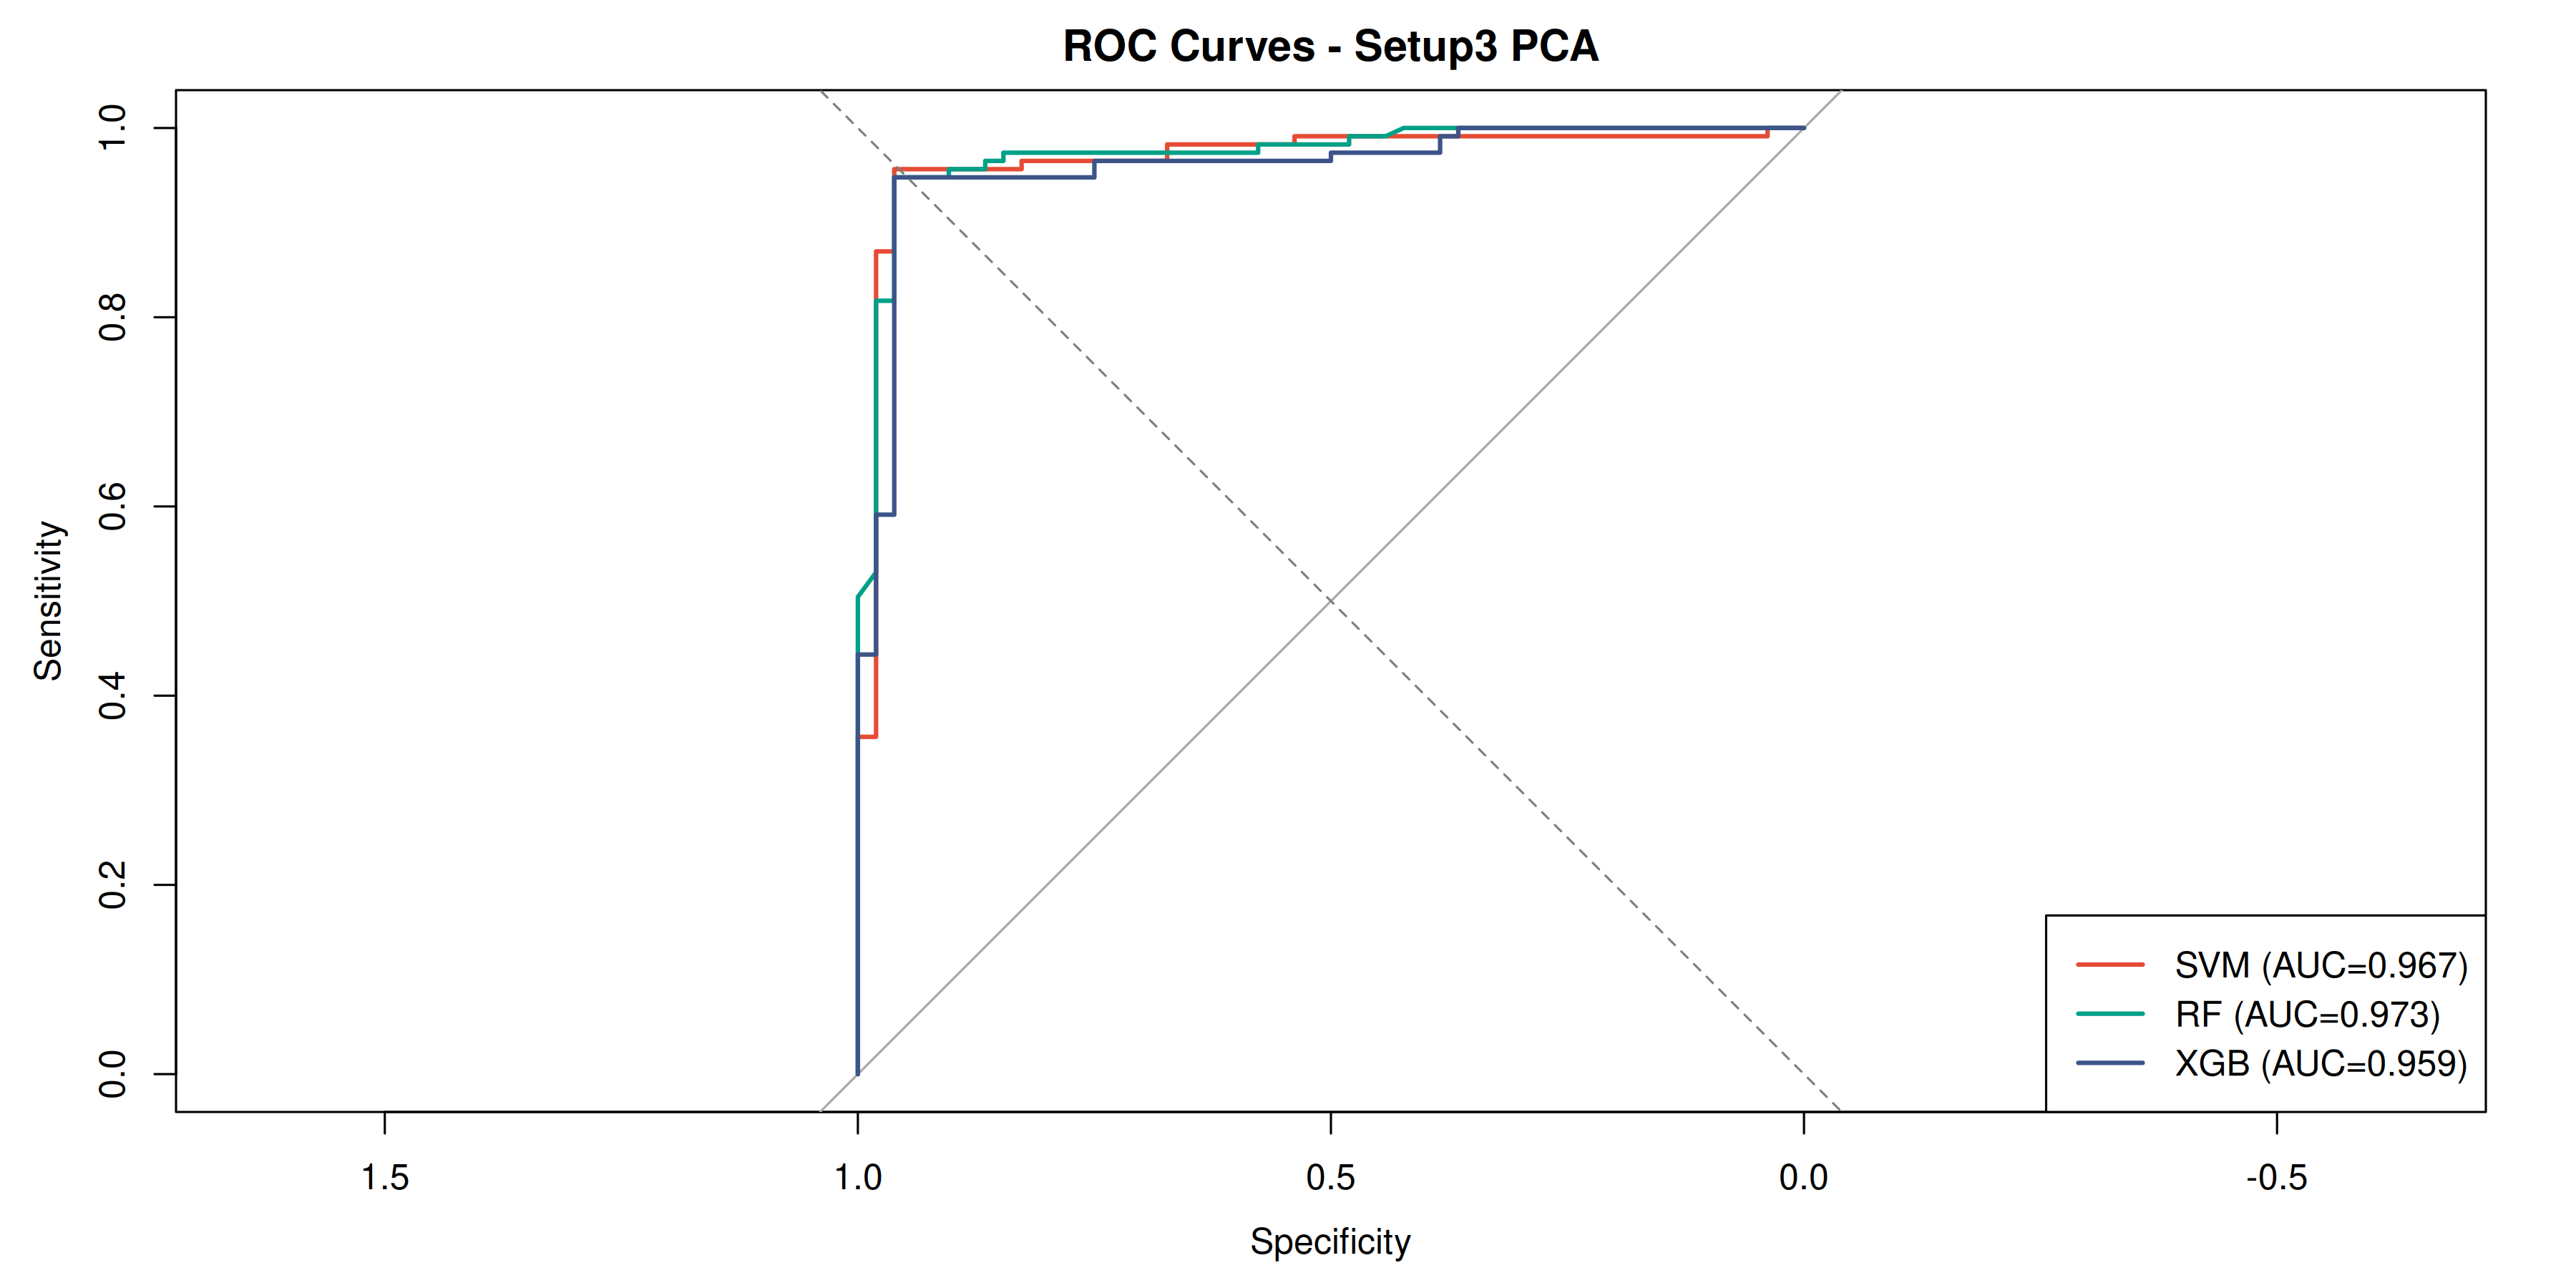
\includegraphics[width=0.85\textwidth]{roc_curves_Setup3_PCA.png}
\caption{PCA ROC eğrileri}
\label{fig:roc3}
\end{figure}

\begin{figure}[H]
\centering
\begin{minipage}{0.32\textwidth}
\centering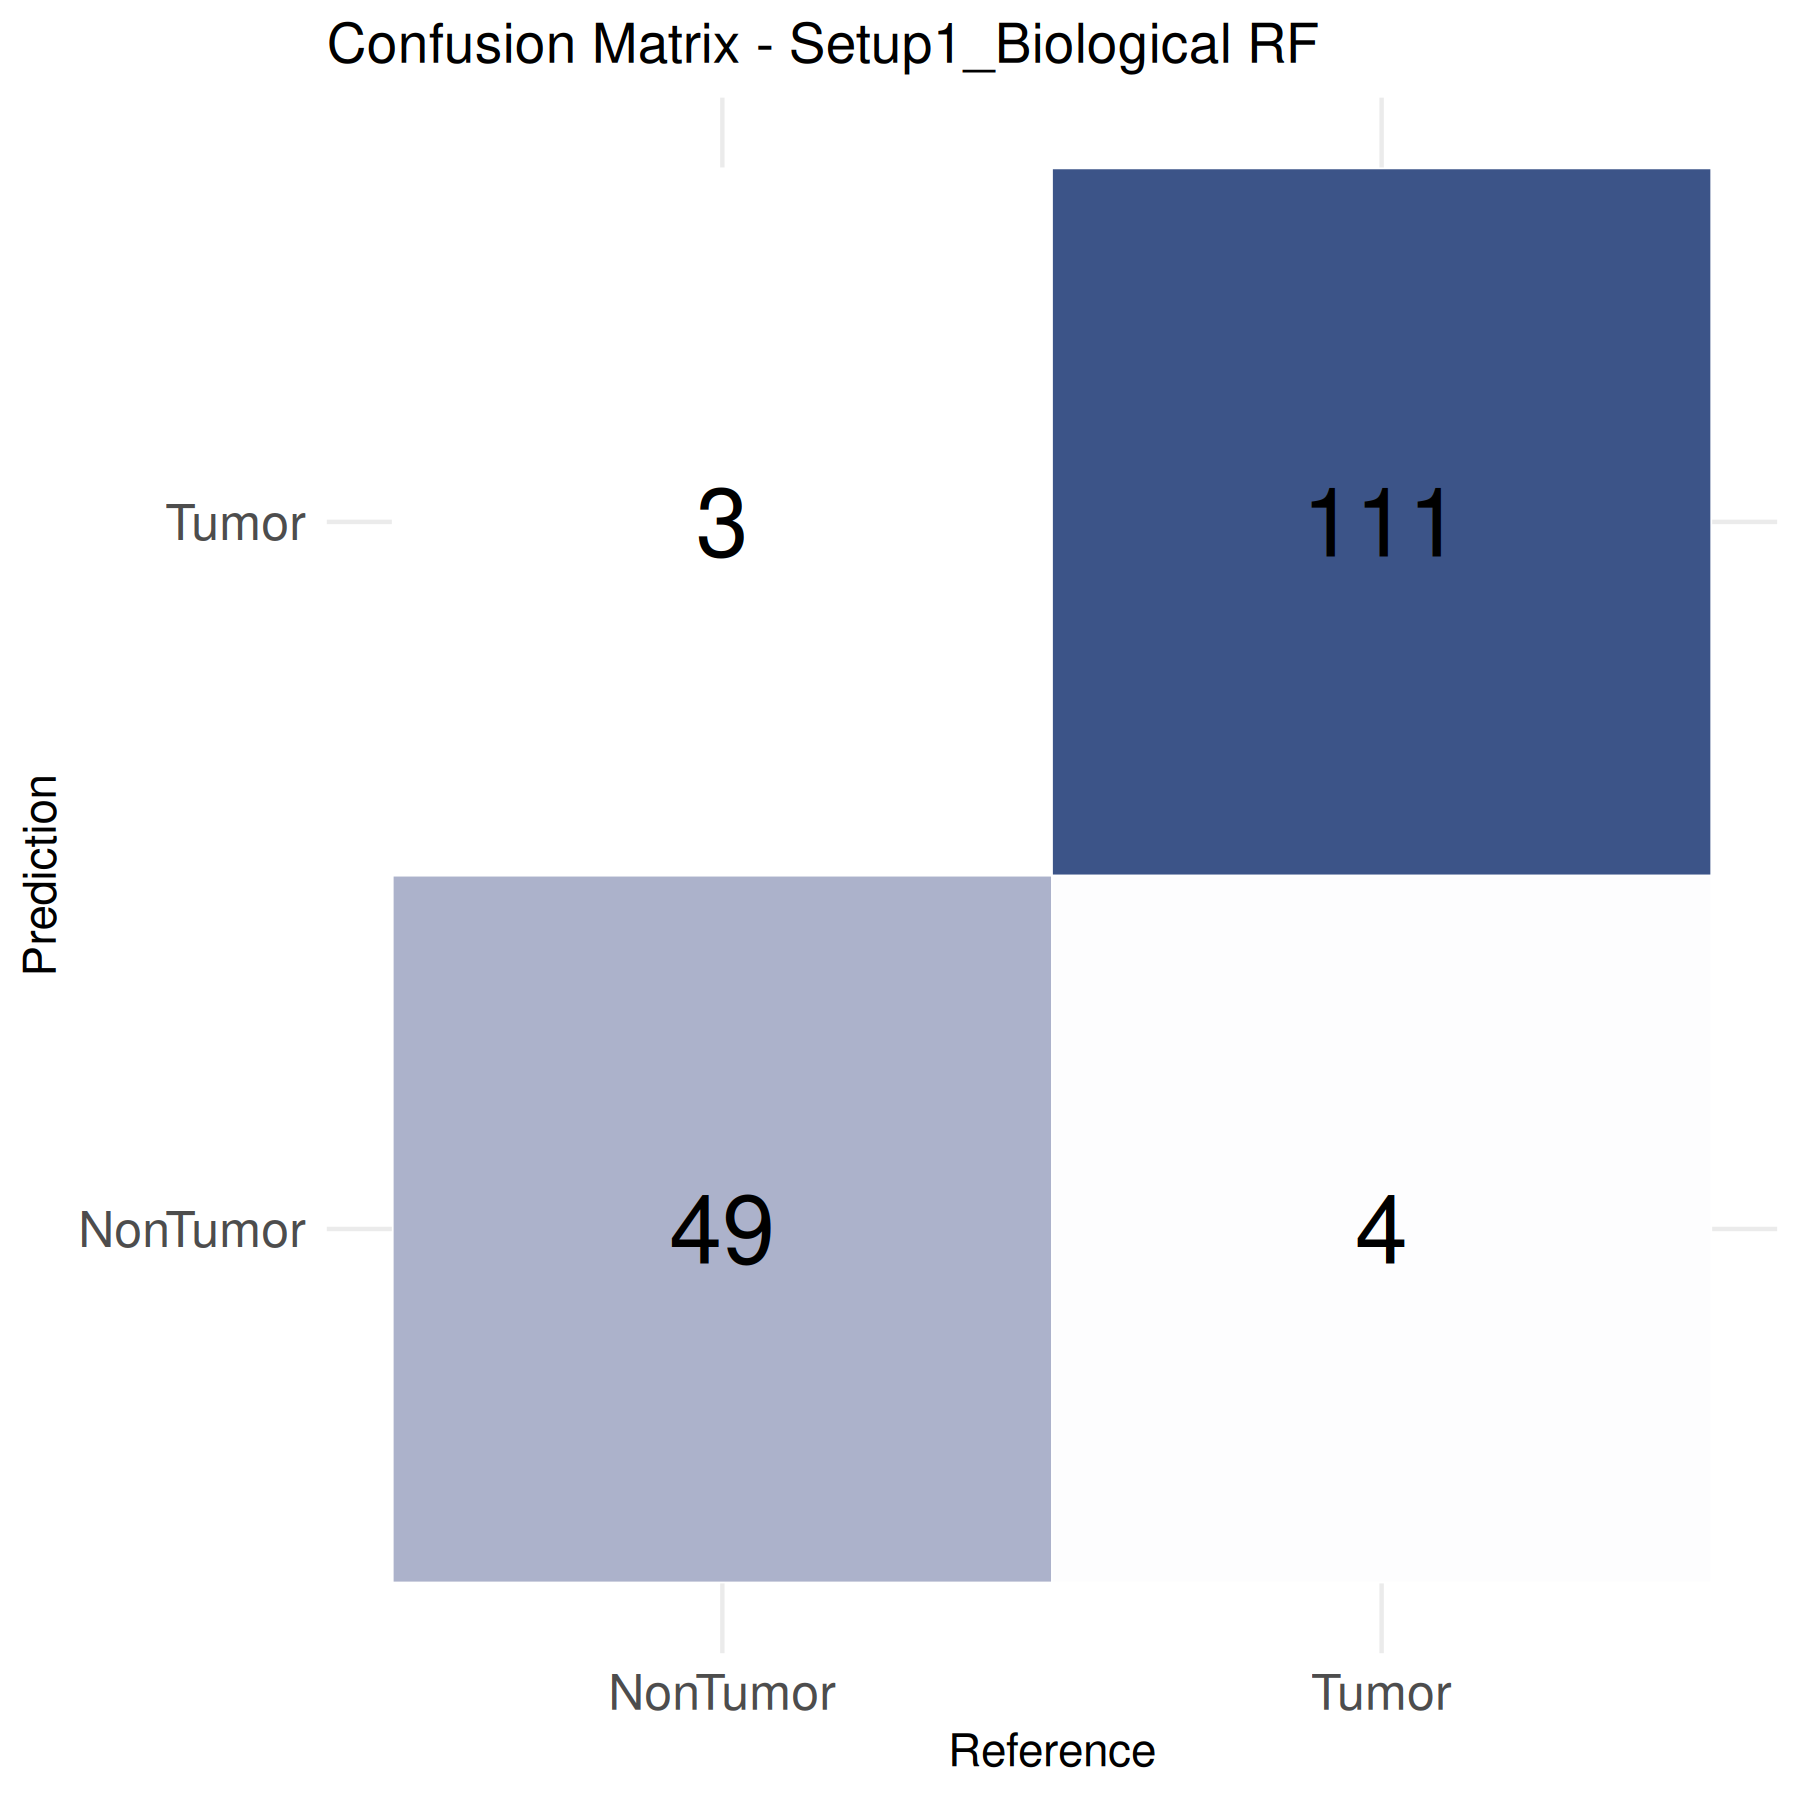
\includegraphics[width=\textwidth]{confusion_matrix_Setup1_Biological_RF.png}
\end{minipage}\hfill
\begin{minipage}{0.32\textwidth}
\centering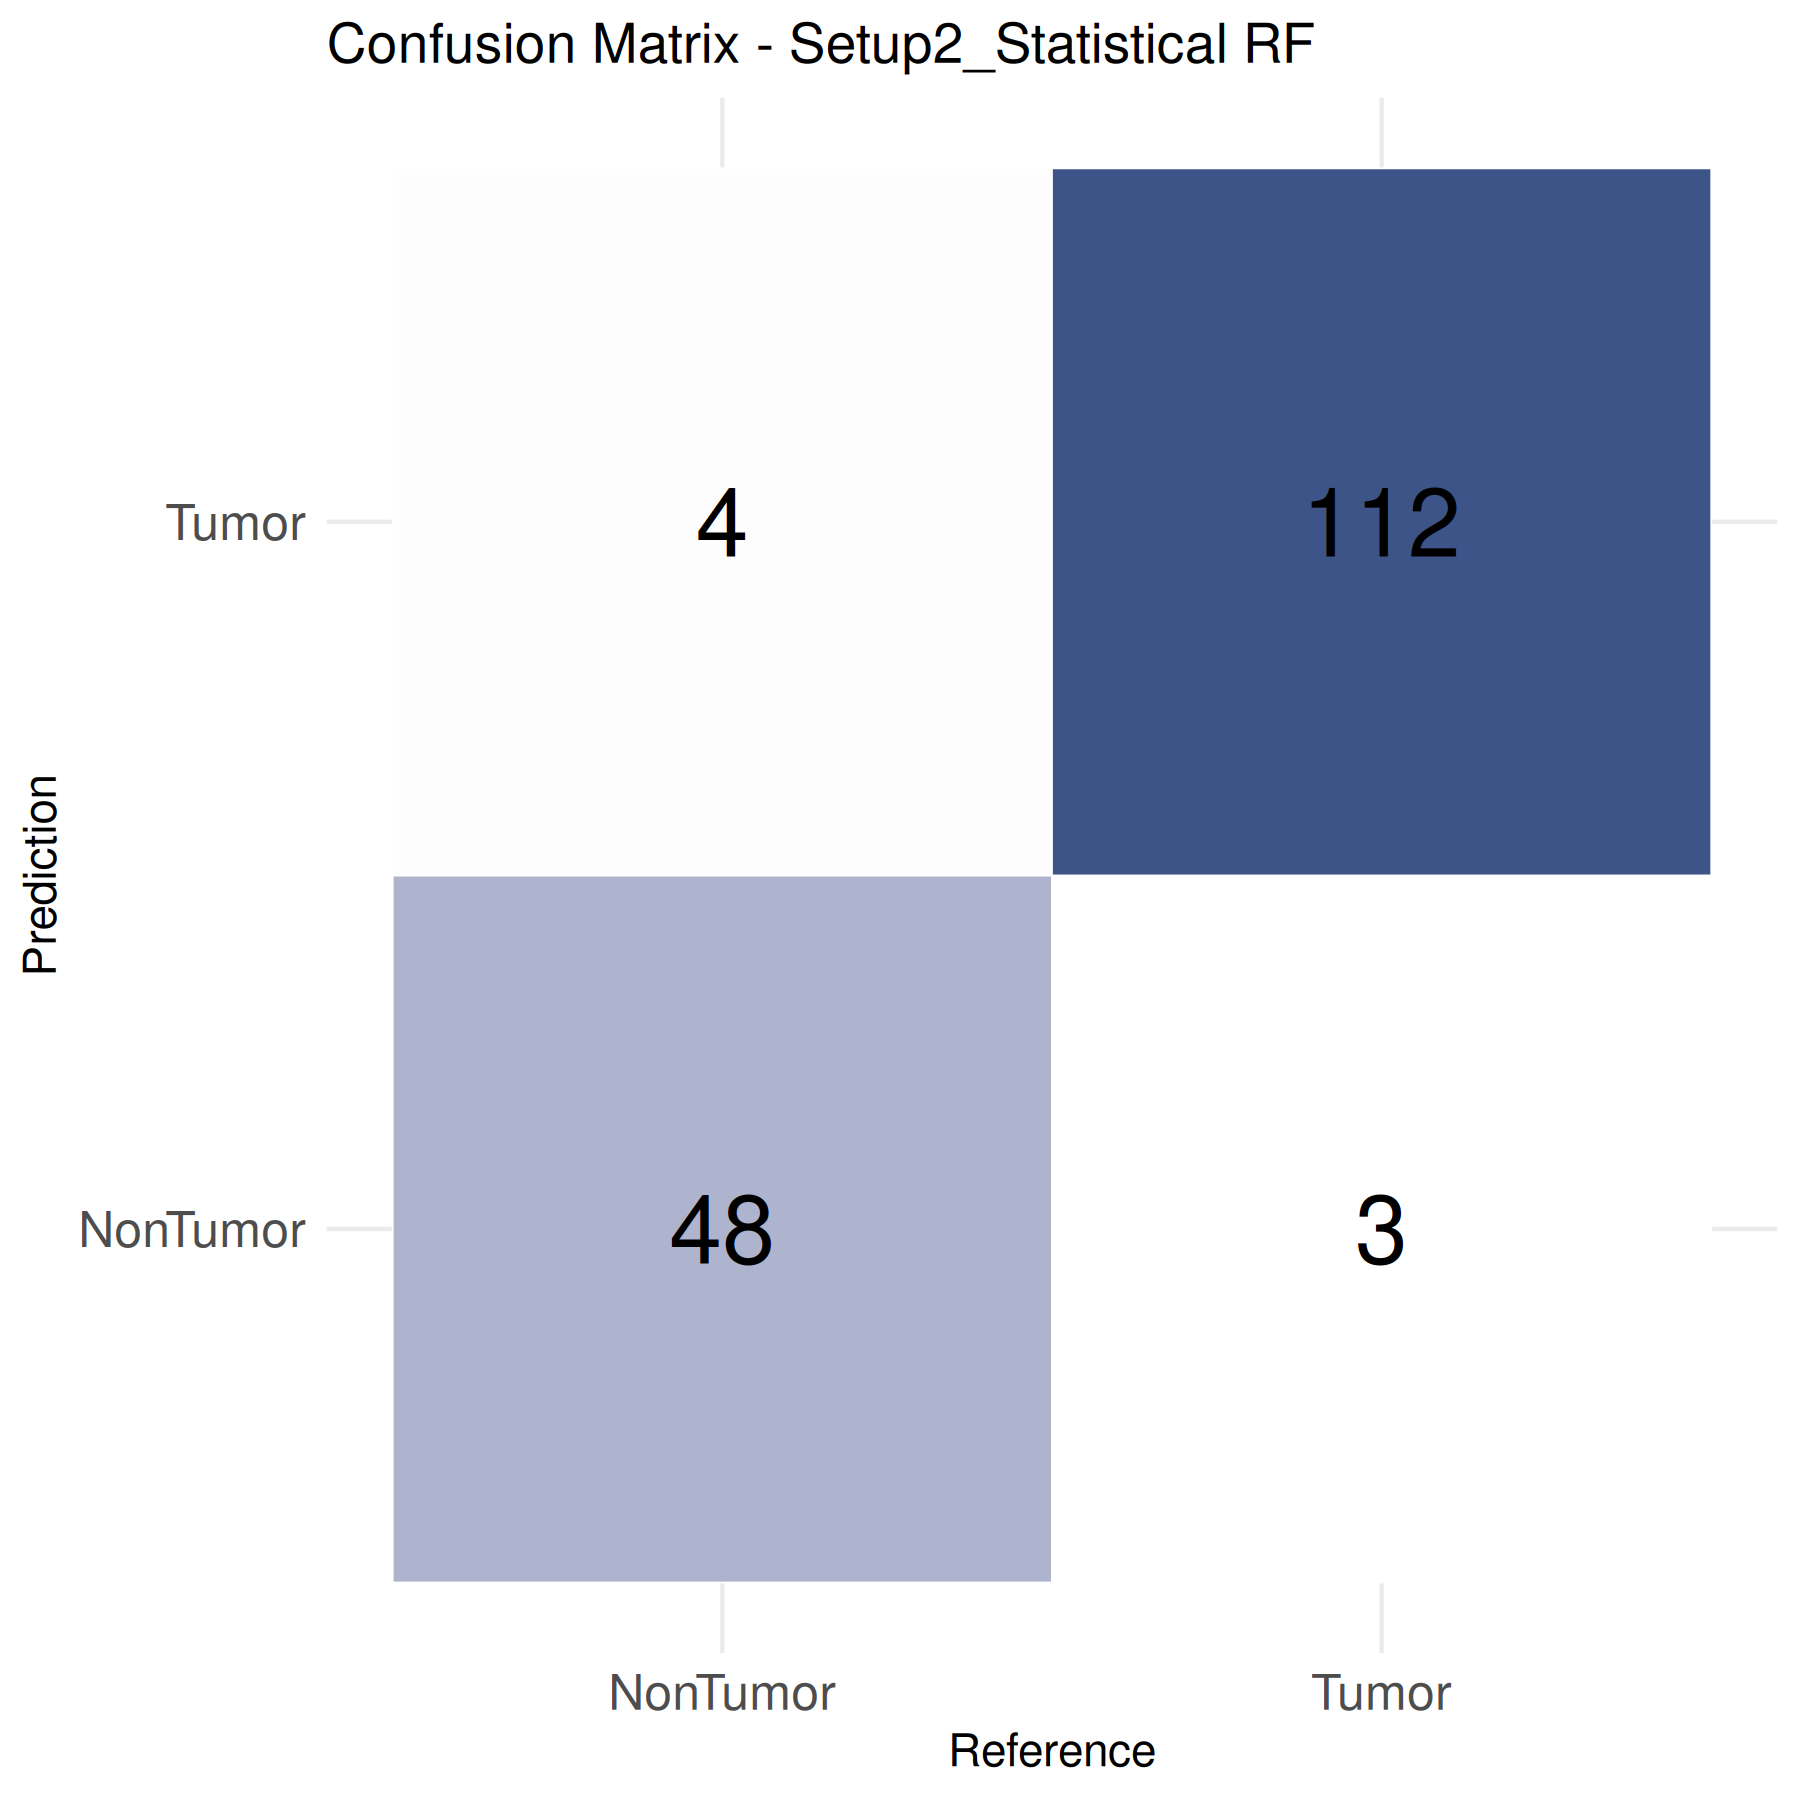
\includegraphics[width=\textwidth]{confusion_matrix_Setup2_Statistical_RF.png}
\end{minipage}\hfill
\begin{minipage}{0.32\textwidth}
\centering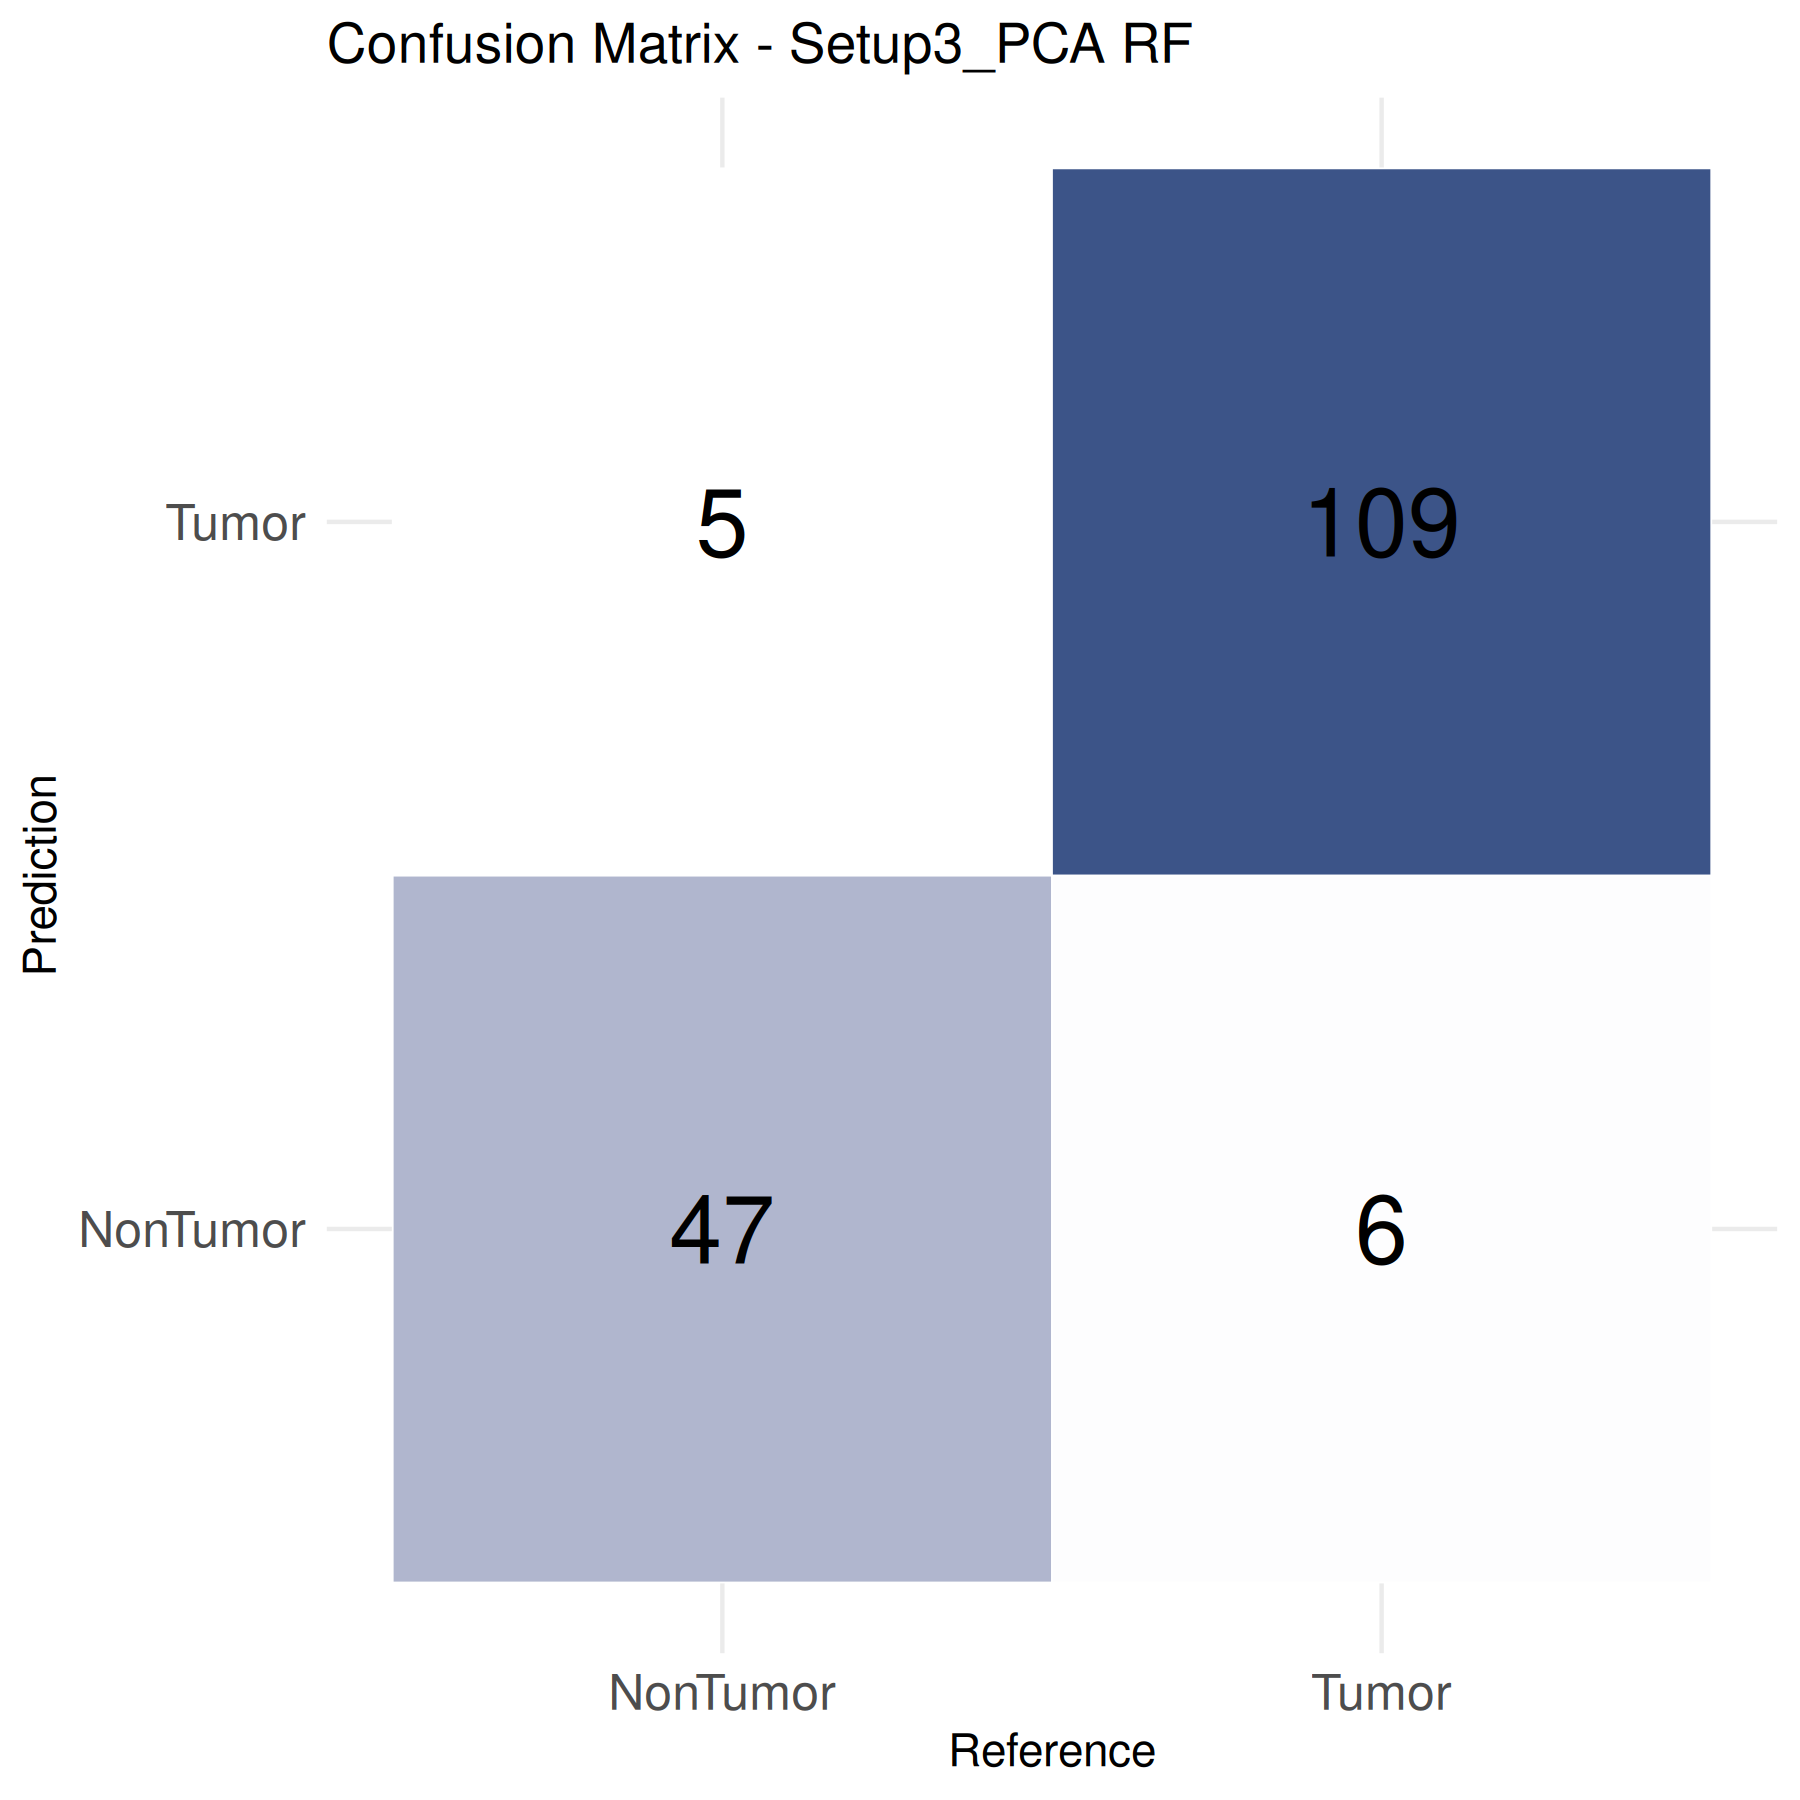
\includegraphics[width=\textwidth]{confusion_matrix_Setup3_PCA_RF.png}
\end{minipage}
\caption{Random Forest karışıklık matrisleri (sırasıyla Biyolojik, İstatistiksel, PCA)}
\label{fig:cm}
\end{figure}

\section{Karşılaştırma ve Yorum}

Biyolojik ve istatistiksel özellik setleri benzer performans göstermiştir. Bu sonuç, DGE ve WGCNA analizleriyle seçilen genlerin tümör/non-tümör ayrımında yararlı bilgiler taşıdığını göstermektedir. PCA tabanlı özellik seti de daha az sayıda bileşen kullanmasına rağmen başarılı sonuçlar vermiştir.

Modeller arasında Random Forest, tüm özellik setlerinde yüksek ve tutarlı AUC değerleri elde etmiştir. En yüksek AUC değeri, istatistiksel özellik seti ile Random Forest modelinde elde edilmiştir (AUC = 0,981).

Değerlendirmede hasta-bazlı çapraz doğrulama kullanıldığı için aynı hastaya ait örneklerin hem eğitim hem test kümesine düşmesi engellenmiştir. Ayrıca PCA kullanılan özellik seti'nde boyut indirgeme işlemi her fold içinde yalnızca eğitim verisi üzerinde yapılmıştır. Bununla birlikte, biyolojik ve istatistiksel gen listeleri tüm veri seti üzerinde belirlendiği için bu iki özellik seti keşifsel karşılaştırma olarak değerlendirilmelidir.

% ------------------------------------------------------------------------------
\chapter{SONUÇLAR}

Bu projede GSE76427 hepatosellüler karsinom veri seti üzerinde gen ifadesi analizi, survival analizi, WGCNA, GO enrichment analizi ve makine öğrenmesi tabanlı sınıflandırma uygulanmıştır. Çalışmada tümör ve non-tümör dokular arasındaki gen ifade farklılıkları incelenmiş, bu farklılıkların biyolojik anlamı değerlendirilmiş ve elde edilen gen listelerinin sınıflandırma başarısına katkısı karşılaştırılmıştır.

Elde edilen başlıca sonuçlar aşağıda özetlenmiştir:

\begin{enumerate}[leftmargin=*]
    \item Diferansiyel gen ifadesi analizi, prob filtreleme ve gen anotasyonu sonrası elde edilen 14.323 benzersiz gen üzerinde gerçekleştirilmiştir. Tümör ve non-tümör dokular arasında 705 gen anlamlı düzeyde farklı ifade göstermiştir. Bu genlerin 216'sı tümör dokusunda daha yüksek, 489'u ise daha düşük ifade edilmiştir.
    
    \item DGE sonuçlarında GPC3, AKR1B10, SPINK1, TOP2A ve ACSL4 tümör dokusunda daha yüksek ifade edilen genler arasında öne çıkmıştır. HAMP, CYP1A2, FCN3, MT1H ve MT1G ise tümör dokusunda daha düşük ifade göstermiştir. Bu sonuçlar, HCC dokusunda bazı tümörle ilişkili genlerin arttığını, buna karşılık normal karaciğer fonksiyonlarıyla ilişkili bazı genlerin azaldığını göstermektedir.
    
    \item Survival analizinde genel sağkalım temel alınmıştır. İncelenen genler arasında MT1G, MT1H ve AKR1B10 Kaplan-Meier analizinde anlamlı sonuçlar göstermiştir. Cox modelinde özellikle yüksek MT1G ifadesi daha yüksek ölüm riskiyle ilişkili bulunmuştur. Bu sonuç, bazı genlerin yalnızca tümör/non-tümör ayrımında değil, tümör örnekleri içinde survival ile ilişkili olabileceğini göstermektedir.
    
    \item WGCNA analizi ile 6 gen modülü belirlenmiştir. Brown modülü, tümör/non-tümör ayrımıyla en güçlü ilişki gösteren modül olarak seçilmiştir. Bu modülde yer alan hub genler, modülü temsil etme gücü ve tümör/non-tümör ayrımıyla ilişkisi dikkate alınarak belirlenmiştir.
    
    \item Brown modülü üzerinde yapılan GO enrichment analizi, bu modüldeki genlerin özellikle küçük molekül metabolizması, amino asit metabolizması ve yağ asidi metabolizması gibi karaciğerin temel görevleriyle ilişkili süreçlerde yoğunlaştığını göstermiştir. Bu bulgu, tümör dokusunda normal karaciğer metabolizmasıyla ilişkili genlerin baskılanabileceği yorumunu desteklemektedir.
    
    \item Makine öğrenmesi aşamasında üç farklı özellik seti ve üç farklı model karşılaştırılmıştır. Biyolojik analizlerle seçilen genler, istatistiksel olarak seçilen genler ve PCA bileşenleri kullanılarak tümör/non-tümör sınıflandırması yapılmıştır. Modeller genel olarak yüksek başarı göstermiştir. En yüksek AUC değeri, istatistiksel özellik seti ile Random Forest modelinde elde edilmiştir.
\end{enumerate}

Genel olarak sonuçlar, HCC tümör dokusunun gen ifade profili bakımından non-tümör dokudan belirgin şekilde ayrıldığını göstermektedir. Tümör dokusunda normal karaciğer metabolizmasıyla ilişkili bazı genlerin daha düşük, tümör gelişimiyle ilişkili bazı genlerin ise daha yüksek ifade edildiği görülmüştür. Bu ifade değişimleri hem biyolojik analizlerde anlamlı örüntüler oluşturmuş hem de makine öğrenmesi modelleriyle tümör/non-tümör ayrımının başarılı şekilde yapılmasını sağlamıştır.


\end{document}